% ============================================================
% ROBIN-FPGA — expert-level IEEEtran paper with embedded TikZ
% Compile: pdflatex robin-fpga.tex (run twice for cross-refs)
% ============================================================
\documentclass[journal,onecolumn=false]{IEEEtran}

% ---- packages ----
\usepackage[utf8]{inputenc}
\usepackage{amsmath, amssymb, amsfonts}
\usepackage{graphicx}
\usepackage{booktabs}
\usepackage{array}
\usepackage{multirow}
\usepackage{xcolor}
\usepackage{tikz}
\usepackage{pgfplots}
\usepackage{pgfplotstable}
\pgfplotsset{compat=1.18}
\usepgfplotslibrary{fillbetween,colormaps,statistics}
\usetikzlibrary{arrows.meta, positioning, shapes.geometric, fit, calc,
  decorations.pathreplacing, backgrounds, shadows, patterns, shadings,
  matrix, chains, scopes, decorations.pathmorphing, intersections, plotmarks}
\usepackage{algorithm}
\usepackage{algpseudocode}
\usepackage{url}
\usepackage[hidelinks]{hyperref}
\usepackage{caption}
\captionsetup[figure]{font=footnotesize, labelfont={bf,sf}, textfont=sf, justification=raggedright, singlelinecheck=false}
\captionsetup[table]{font=footnotesize, labelfont={bf,sf}, textfont=sf}

% ============================================================
% PALETTE
% ============================================================
\definecolor{robinblue}{HTML}{2E5C8A}
\definecolor{robinmid}{HTML}{4A90B5}
\definecolor{robinlight}{HTML}{7CB7CC}
\definecolor{robinrust}{HTML}{C2410C}
\definecolor{robinamber}{HTML}{F59E0B}
\definecolor{robinteal}{HTML}{0F766E}
\definecolor{robingrey}{HTML}{525252}
\definecolor{robinbg}{HTML}{F5F5F5}
\definecolor{robingreen}{HTML}{15803D}
\definecolor{robinred}{HTML}{B91C1C}
\definecolor{robinpurple}{HTML}{6D28D9}
\definecolor{dieblue}{HTML}{1E3A5F}
\definecolor{bramcol}{HTML}{6366F1}
\definecolor{dspcol}{HTML}{F59E0B}
\definecolor{uramcol}{HTML}{8B5CF6}
\definecolor{aiecol}{HTML}{059669}
\definecolor{ioring}{HTML}{475569}
\definecolor{noccol}{HTML}{DC2626}
\definecolor{hbmcol}{HTML}{0EA5E9}
\definecolor{pciecol}{HTML}{EC4899}

% ============================================================
% MACRO: FPGA fabric (full version with all features)
% ============================================================
\newcommand{\drawFPGA}[1][1.0]{%
\begin{scope}[scale=#1, transform shape]
  \draw[rounded corners=3pt, fill=robingrey!12, draw=robingrey!70, line width=0.7pt]
        (-0.25,-0.25) rectangle (5.45,4.85);
  \draw[rounded corners=2pt, fill=dieblue!8, draw=dieblue, line width=0.5pt]
        (0,0) rectangle (5.2,4.6);
  \fill[aiecol!18] (0.1,3.8) rectangle (5.1,4.5);
  \draw[aiecol!70, line width=0.25pt] (0.1,3.8) rectangle (5.1,4.5);
  \foreach \x in {0,...,14}{
    \foreach \y in {0,1}{
      \fill[aiecol!75, draw=aiecol!90!black, line width=0.1pt]
        ({0.18+\x*0.33},{3.88+\y*0.3}) rectangle ({0.45+\x*0.33},{4.13+\y*0.3});
    }
  }
  \node[font=\tiny\sffamily, aiecol!70!black] at (2.6,4.66) {AIE-ML tile array};
  \draw[ioring!80, line width=1pt, rounded corners=1pt]
        (0.15,0.15) rectangle (5.05,3.7);
  \foreach \x in {0,...,14}{
    \foreach \y in {0,...,8}{
      \pgfmathsetmacro{\d}{((\x-7)*(\x-7) + (\y-4)*(\y-4))/40}
      \pgfmathsetmacro{\u}{max(0, 0.95 - \d)}
      \pgfmathsetmacro{\rr}{min(1.0, 0.55 + 0.45*\u)}
      \pgfmathsetmacro{\gg}{max(0.30, 0.95 - 0.65*\u)}
      \pgfmathsetmacro{\bb}{max(0.25, 0.60 - 0.30*\u)}
      \definecolor{clb}{rgb}{\rr,\gg,\bb}
      \fill[clb, draw=clb!60!black, line width=0.05pt]
        ({0.32+\x*0.32},{0.32+\y*0.36}) rectangle
        ({0.55+\x*0.32},{0.55+\y*0.36});
    }
  }
  \foreach \cx in {3,8,12}{
    \fill[bramcol, draw=bramcol!50!black, line width=0.15pt]
      ({0.30+\cx*0.32 - 0.04},0.30) rectangle ({0.30+\cx*0.32 + 0.20},3.50);
  }
  \foreach \cx in {5,10}{
    \fill[dspcol, draw=dspcol!60!black, line width=0.15pt]
      ({0.30+\cx*0.32 - 0.04},0.30) rectangle ({0.30+\cx*0.32 + 0.20},3.50);
  }
  \fill[uramcol, draw=uramcol!50!black, line width=0.15pt]
        ({0.30+13*0.32 - 0.04},0.30) rectangle ({0.30+13*0.32 + 0.20},3.50);
  \draw[noccol!90, line width=1.0pt, dash pattern=on 2pt off 1pt]
        (0.15,1.95) -- (5.05,1.95);
  \draw[noccol!90, line width=1.0pt, dash pattern=on 2pt off 1pt]
        (2.6,0.15) -- (2.6,3.7);
  \fill[hbmcol!75, draw=hbmcol!50!black, line width=0.25pt, rounded corners=1pt]
        (-0.22,0.9) rectangle (-0.04,2.8);
  \node[font=\tiny\sffamily, hbmcol!60!black, rotate=90] at (-0.13,1.85) {HBM2e};
  \fill[pciecol!75, draw=pciecol!50!black, line width=0.25pt, rounded corners=1pt]
        (5.24,0.9) rectangle (5.42,2.8);
  \node[font=\tiny\sffamily, pciecol!60!black, rotate=90] at (5.33,1.85) {GTM/PCIe};
\end{scope}
}

% Compact FPGA chip (small, for inline use)
\newcommand{\drawFPGAsmall}[1][1.0]{%
\begin{scope}[scale=#1, transform shape]
  \draw[rounded corners=1pt, fill=dieblue!15, draw=dieblue, line width=0.4pt]
        (0,0) rectangle (1.6,1.4);
  \fill[aiecol!50, draw=aiecol!80!black, line width=0.2pt] (0.1,1.15) rectangle (1.5,1.35);
  \foreach \cx in {0.35,0.7,1.05}{
    \fill[bramcol!75] (\cx,0.2) rectangle ({\cx+0.07},1.1);
  }
  \foreach \xx in {0,...,7}{
    \foreach \yy in {0,...,4}{
      \pgfmathsetmacro{\u}{rand}
      \pgfmathsetmacro{\rr}{0.55 + 0.45*(\u+1)/2}
      \pgfmathsetmacro{\gg}{0.92 - 0.55*(\u+1)/2}
      \pgfmathsetmacro{\bb}{0.4}
      \definecolor{cc}{rgb}{\rr,\gg,\bb}
      \fill[cc] ({0.15+\xx*0.17},{0.22+\yy*0.18}) rectangle ({0.22+\xx*0.17},{0.32+\yy*0.18});
    }
  }
  \draw[noccol!80, line width=0.4pt, dash pattern=on 1pt off 0.5pt]
        (0.1,0.65) -- (1.5,0.65);
\end{scope}
}

% ============================================================
% MACRO: stacked FPGAs (K parallel runs)
% ============================================================
\newcommand{\drawFPGAStack}[1][1.0]{%
\begin{scope}[scale=#1, transform shape]
  \foreach \i in {4,3,2,1,0}{
    \begin{scope}[shift={(\i*0.32,\i*-0.20)}]
      \drawFPGAsmall[0.85]
    \end{scope}
  }
\end{scope}
}

% ============================================================
% MACRO: RL agent neural network (policy + value heads)
% ============================================================
\newcommand{\drawAgentNN}[1][1.0]{%
\begin{scope}[scale=#1, transform shape]
  \draw[rounded corners=2pt, fill=robinamber!12, draw=robinrust, line width=0.6pt]
        (-0.15,-0.20) rectangle (4.6,3.45);
  \node[font=\scriptsize\sffamily\bfseries, robinrust] at (2.225,3.18) {DR-PPO agent $\pi_\theta\,/\,V_\phi$};
  \foreach \y in {0,1,2,3,4}{
    \fill[robinmid] (0.3,{0.4+\y*0.55}) circle (0.13);
  }
  \node[font=\tiny\sffamily, robinmid!50!black] at (0.3,0.0) {$z_t$};
  \foreach \y in {0,1,2,3,4,5}{
    \fill[robinblue] (1.4,{0.25+\y*0.5}) circle (0.13);
  }
  \foreach \y in {0,1,2,3,4,5}{
    \fill[robinblue!80] (2.5,{0.25+\y*0.5}) circle (0.13);
  }
  \foreach \i in {0,...,4}{
    \foreach \j in {0,...,5}{
      \pgfmathsetmacro{\op}{0.10 + 0.30*(rand+1)/2}
      \draw[robingrey, line width=0.12pt, opacity=\op]
           (0.3,{0.4+\i*0.55}) -- (1.4,{0.25+\j*0.5});
    }
  }
  \foreach \i in {0,...,5}{
    \foreach \j in {0,...,5}{
      \pgfmathsetmacro{\op}{0.10 + 0.30*(rand+1)/2}
      \draw[robingrey, line width=0.12pt, opacity=\op]
           (1.4,{0.25+\i*0.5}) -- (2.5,{0.25+\j*0.5});
    }
  }
  \draw[robinrust, line width=0.5pt, fill=white] (3.4,1.85) rectangle (4.45,3.0);
  \node[font=\tiny\sffamily\bfseries, robinrust] at (3.925,3.12) {$\pi(a|z)$};
  \foreach \i/\h in {0/0.70, 1/0.95, 2/0.35, 3/0.55, 4/0.20}{
    \fill[robinrust!80] ({3.5+\i*0.20},1.9) rectangle ({3.65+\i*0.20},{1.9+\h*0.95});
  }
  \draw[robingreen, line width=0.5pt, fill=white] (3.4,0.4) rectangle (4.45,1.4);
  \node[font=\tiny\sffamily\bfseries, robingreen] at (3.925,1.52) {$V_\phi(z)$};
  \fill[robingreen!70] (3.925,0.9) circle (0.22);
  \node[font=\tiny\sffamily, white] at (3.925,0.9) {$V$};
  \foreach \i in {0,...,5}{
    \draw[robingrey, line width=0.15pt, opacity=0.3]
         (2.5,{0.25+\i*0.5}) -- (3.4,2.4);
    \draw[robingrey, line width=0.15pt, opacity=0.3]
         (2.5,{0.25+\i*0.5}) -- (3.4,0.9);
  }
\end{scope}
}

% ============================================================
% MACRO: Timing graph DAG with critical path
% ============================================================
\newcommand{\drawTimingGraph}[1][1.0]{%
\begin{scope}[scale=#1, transform shape]
  \draw[rounded corners=2pt, fill=robinbg, draw=robinblue!60, line width=0.5pt]
        (-0.15,-0.20) rectangle (3.95,2.85);
  \node[font=\scriptsize\sffamily\bfseries, robinblue] at (1.9,2.6) {Timing graph $G_t$};
  \node[circle, fill=robingreen!70, draw=robingreen, line width=0.3pt,
        inner sep=0.6pt, font=\tiny\sffamily, text=white] (n0) at (0.3,1.2) {FF};
  \node[circle, fill=robingreen!50, draw=robingreen, line width=0.3pt,
        inner sep=0.6pt, font=\tiny\sffamily, text=white] (n1a) at (1.1,2.0) {L};
  \node[circle, fill=robinamber!40!white, draw=robinamber, line width=0.4pt,
        inner sep=0.6pt, font=\tiny\sffamily, text=robingrey] (n1b) at (1.1,1.2) {L};
  \node[circle, fill=robinred!75, draw=robinred, line width=0.4pt,
        inner sep=0.6pt, font=\tiny\sffamily, text=white] (n1c) at (1.1,0.4) {L};
  \node[circle, fill=robingreen!50, draw=robingreen, line width=0.3pt,
        inner sep=0.6pt, font=\tiny\sffamily, text=white] (n2a) at (2.0,1.8) {L};
  \node[circle, fill=robinred!80, draw=robinred, line width=0.5pt,
        inner sep=0.6pt, font=\tiny\sffamily, text=white] (n2b) at (2.0,0.9) {L};
  \node[circle, fill=robinamber!40!white, draw=robinamber, line width=0.3pt,
        inner sep=0.6pt, font=\tiny\sffamily, text=robingrey] (n2c) at (2.0,0.1) {L};
  \node[circle, fill=robingreen!60, draw=robingreen, line width=0.3pt,
        inner sep=0.6pt, font=\tiny\sffamily, text=white] (n3a) at (2.9,1.5) {L};
  \node[circle, fill=robinred!85, draw=robinred, line width=0.5pt,
        inner sep=0.6pt, font=\tiny\sffamily, text=white] (n3b) at (2.9,0.6) {L};
  \node[circle, fill=robingreen!70, draw=robingreen, line width=0.3pt,
        inner sep=0.6pt, font=\tiny\sffamily, text=white] (nE) at (3.6,1.2) {FF};
  \draw[robingrey, line width=0.25pt, -Latex] (n0)--(n1a);
  \draw[robingrey, line width=0.25pt, -Latex] (n0)--(n1b);
  \draw[robingrey, line width=0.25pt, -Latex] (n1a)--(n2a);
  \draw[robingrey, line width=0.25pt, -Latex] (n1b)--(n2a);
  \draw[robingrey, line width=0.25pt, -Latex] (n1b)--(n2c);
  \draw[robingrey, line width=0.25pt, -Latex] (n2a)--(n3a);
  \draw[robingrey, line width=0.25pt, -Latex] (n2c)--(n3b);
  \draw[robingrey, line width=0.25pt, -Latex] (n3a)--(nE);
  \draw[robinred, line width=0.7pt, -Latex] (n0)--(n1c);
  \draw[robinred, line width=0.7pt, -Latex] (n1c)--(n2b);
  \draw[robinred, line width=0.7pt, -Latex] (n2b)--(n3b);
  \draw[robinred, line width=0.7pt, -Latex] (n3b)--(nE);
  \node[font=\tiny\sffamily, robinred!90!black] at (1.9,-0.10) {critical path:\ WNS$=-0.12$ns};
\end{scope}
}

% ============================================================
% MACRO: Code editor window (HLS C++)
% ============================================================
\newcommand{\drawCodeWindow}[1][1.0]{%
\begin{scope}[scale=#1, transform shape]
  \draw[rounded corners=2pt, fill=robinbg, draw=robingrey!60, line width=0.4pt]
        (0,0) rectangle (4.0,2.65);
  \fill[robingrey!25, rounded corners=2pt] (0,2.30) rectangle (4.0,2.65);
  \fill[robinred!80] (0.18,2.48) circle (0.08);
  \fill[robinamber!80] (0.42,2.48) circle (0.08);
  \fill[robingreen!80] (0.66,2.48) circle (0.08);
  \node[font=\tiny\sffamily, robingrey!80!black] at (2.0,2.47) {kernel\_gemm.cpp};
  \node[font=\tiny\ttfamily, anchor=west, robinpurple]      at (0.10,2.05) {\#pragma};
  \node[font=\tiny\ttfamily, anchor=west, robinblue]        at (0.72,2.05) {HLS PIPELINE II=1};
  \node[font=\tiny\ttfamily, anchor=west, robinpurple]      at (0.10,1.80) {void};
  \node[font=\tiny\ttfamily, anchor=west, robinrust]        at (0.45,1.80) {gemm};
  \node[font=\tiny\ttfamily, anchor=west, robingrey!85!black] at (0.85,1.80) {(a,b,c)\ \{};
  \node[font=\tiny\ttfamily, anchor=west, robinpurple]      at (0.30,1.55) {for};
  \node[font=\tiny\ttfamily, anchor=west, robingrey!85!black] at (0.55,1.55) {(int i=0; i<N; ++i)\ \{};
  \node[font=\tiny\ttfamily, anchor=west, robinpurple]      at (0.50,1.30) {\#pragma};
  \node[font=\tiny\ttfamily, anchor=west, robinblue]        at (1.12,1.30) {HLS UNROLL};
  \node[font=\tiny\ttfamily, anchor=west, robinpurple]      at (0.50,1.05) {for};
  \node[font=\tiny\ttfamily, anchor=west, robingrey!85!black] at (0.75,1.05) {(int j=0; j<N; ++j)};
  \node[font=\tiny\ttfamily, anchor=west, robingrey!85!black] at (0.70,0.80) {c[i][j] += a[i][k]};
  \node[font=\tiny\ttfamily, anchor=west, robingrey!85!black] at (0.70,0.55) {\quad\ \ \ \ \,* b[k][j];};
  \node[font=\tiny\ttfamily, anchor=west, robingrey!85!black] at (0.30,0.30) {\}};
  \node[font=\tiny\ttfamily, anchor=west, robingrey!85!black] at (0.10,0.10) {\}};
\end{scope}
}

% ============================================================
% MACRO: Return distribution histogram with CVaR tail
% ============================================================
\newcommand{\drawRewardHist}[1][1.0]{%
\begin{scope}[scale=#1, transform shape]
  \draw[rounded corners=2pt, fill=robinbg, draw=robinrust!60, line width=0.5pt]
        (-0.15,-0.15) rectangle (3.55,2.55);
  \node[font=\scriptsize\sffamily\bfseries, robinrust] at (1.7,2.28) {Return dist.\,$R_{k,\theta}$};
  \draw[-Latex, robingrey!70, line width=0.3pt] (0.2,0.2) -- (3.30,0.2);
  \draw[-Latex, robingrey!70, line width=0.3pt] (0.2,0.2) -- (0.2,2.00);
  \node[font=\tiny\sffamily, anchor=east] at (0.2,1.88) {density};
  \node[font=\tiny\sffamily, anchor=west] at (3.20,0.2) {$R$};
  \foreach \i/\h in {0/0.10, 1/0.18, 2/0.32, 3/0.50, 4/0.70, 5/0.92, 6/1.20, 7/1.45, 8/1.30, 9/1.00, 10/0.68, 11/0.40, 12/0.20}{
    \pgfmathsetmacro{\x}{0.35 + \i*0.22}
    \fill[robinblue!50, draw=robinblue!80, line width=0.15pt] (\x,0.2) rectangle ({\x+0.18},{0.2+\h});
  }
  \foreach \i/\h in {0/0.10, 1/0.18, 2/0.32, 3/0.50}{
    \pgfmathsetmacro{\x}{0.35 + \i*0.22}
    \fill[robinrust!85, draw=robinrust, line width=0.15pt] (\x,0.2) rectangle ({\x+0.18},{0.2+\h});
  }
  \draw[robinrust, line width=0.5pt, dashed] (1.23,0.2) -- (1.23,2.00);
  \node[font=\tiny\sffamily, robinrust, anchor=south] at (1.23,2.00) {VaR$_{0.2}$};
  \node[font=\tiny\sffamily\bfseries, robinrust] at (0.7,0.70) {CVaR$_\beta$};
\end{scope}
}

% ============================================================
% MACRO: Conformal envelope visualization
% ============================================================
\newcommand{\drawConformalEnv}[1][1.0]{%
\begin{scope}[scale=#1, transform shape]
  \draw[rounded corners=2pt, fill=robinbg, draw=robingreen!60, line width=0.5pt]
        (-0.15,-0.15) rectangle (3.55,2.55);
  \node[font=\scriptsize\sffamily\bfseries, robingreen] at (1.7,2.28) {Conformal sign-off $\mathcal{C}_{1-\alpha}$};
  \draw[-Latex, robingrey!70, line width=0.3pt] (0.2,0.4) -- (3.30,0.4);
  \draw[-Latex, robingrey!70, line width=0.3pt] (0.2,0.4) -- (0.2,2.10);
  \node[font=\tiny\sffamily, anchor=west] at (3.20,0.4) {test point $z$};
  \node[font=\tiny\sffamily, anchor=east] at (0.2,2.00) {WNS};
  \draw[robingrey, line width=0.25pt, dashed] (0.2,1.15) -- (3.20,1.15);
  \node[font=\tiny\sffamily, anchor=west, robingrey!80!black] at (3.05,1.05) {$0$};
  \fill[robingreen!25, draw=robingreen!50, line width=0.3pt]
        plot[smooth] coordinates {(0.4,1.65) (0.9,1.58) (1.5,1.72) (2.0,1.55) (2.6,1.60) (3.0,1.55)} --
        plot[smooth] coordinates {(3.0,1.00) (2.6,1.05) (2.0,0.98) (1.5,1.18) (0.9,1.04) (0.4,1.10)} -- cycle;
  \draw[robingreen, line width=0.7pt, smooth]
        plot coordinates {(0.4,1.38) (0.9,1.31) (1.5,1.45) (2.0,1.27) (2.6,1.32) (3.0,1.28)};
  \foreach \x/\y in {0.5/1.42, 1.1/1.25, 1.7/1.55, 2.3/1.20, 2.8/1.30}{
    \fill[robingreen!80!black] (\x,\y) circle (0.05);
  }
  \node[font=\tiny\sffamily, robingreen!80!black] at (1.7,0.65) {accept iff lower $\geq 0$};
\end{scope}
}

% ============================================================
% MACRO: Tool icon (Vivado/Quartus terminal-style)
% ============================================================
\newcommand{\drawToolIcon}[2]{% #1=color #2=label
  \begin{scope}
    \draw[rounded corners=1.5pt, fill=#1!12, draw=#1, line width=0.4pt]
          (0,0) rectangle (1.6,0.85);
    \fill[#1!30, rounded corners=1pt] (0,0.62) rectangle (1.6,0.85);
    \fill[#1!90] (0.1,0.735) circle (0.045);
    \fill[#1!70] (0.22,0.735) circle (0.045);
    \fill[#1!50] (0.34,0.735) circle (0.045);
    \node[font=\tiny\ttfamily, anchor=west, #1!70!black] at (0.1,0.42) {\$ \texttt{\detokenize{tcl>}}};
    \node[font=\tiny\sffamily\bfseries, #1!90!black, anchor=west] at (0.1,0.18) {#2};
  \end{scope}
}

% ============================================================
% MACRO: Reporting card (gauge / metric display)
% ============================================================
\newcommand{\drawGauge}[3]{% #1=label #2=value (0-1) #3=color
  \begin{scope}
    \draw[#3, line width=0.6pt, fill=#3!12] (0,0) circle (0.45);
    \pgfmathsetmacro{\ang}{180*(1-#2)}
    \fill[#3] (0,0) -- ({0.42*cos(\ang)},{0.42*sin(\ang)}) arc[radius=0.42, start angle=\ang, end angle=180] -- cycle;
    \node[font=\tiny\sffamily\bfseries, #3!90!black] at (0,-0.18) {#1};
    \node[font=\scriptsize\sffamily\bfseries, white] at (0,0.12) {#2};
  \end{scope}
}

% =====================================================================
% TITLE / AUTHOR
% =====================================================================
\title{\textsc{Robin-FPGA}: Distributionally-Robust Reinforcement Learning with Conformal Sign-off for FPGA Timing Closure}

\author{Saher~Elsayed,~\IEEEmembership{Member,~IEEE}%
  \thanks{S.~Elsayed is with Altera, San Jose, CA 95134, USA, and with the Department of Computer and Information Science, University of Pennsylvania, Philadelphia, PA 19104, USA (e-mail: selsayed@seas.upenn.edu). ORCID:\,0009-0007-7672-264X.}%
  \thanks{Manuscript prepared May 15, 2026.}}

\markboth{IEEE Transactions on Computer-Aided Design of Integrated Circuits and Systems, vol.~XX, no.~Y, Month~2026}%
{Elsayed: \textsc{Robin-FPGA}: Distributionally-Robust RL with Conformal Sign-off for FPGA Timing Closure}

\begin{document}
\maketitle

% =====================================================================
% ABSTRACT
% =====================================================================
\begin{abstract}
Modern FPGA timing closure is dominated by long, non-deterministic place-and-route (P\&R) iterations whose Worst Negative Slack (WNS) outcomes are highly sensitive to placer seed, process--voltage--temperature (PVT) corner, and tool minor version. Existing machine-learning-for-EDA methods improve mean Quality of Results (QoR) but rarely characterize their own reliability under tool stochasticity, leaving designers without a statistical sign-off envelope. We present \textsc{Robin-FPGA}, an algorithm--toolchain co-designed framework that performs robust design-space exploration for FPGA timing closure. \textsc{Robin-FPGA} couples (i) a graph-attention encoder over the post-synthesis timing graph with a tabular feature head; (ii) a Distributionally-Robust Proximal Policy Optimization (DR-PPO) agent that hedges against P\&R seed variance via a Conditional-Value-at-Risk (CVaR) shaped advantage; and (iii) a split-conformal head that wraps the trained policy with a calibrated upper bound on residual WNS risk at confidence $1{-}\alpha$. We evaluate on a benchmark of $14$ RTL and HLS designs spanning DSP, AI, graph, control, sort/search, and crypto workload classes, across AMD Versal AI Edge and Intel Agilex~7 devices, against vendor defaults, Vivado \texttt{Performance\_Explore}, a TuRBO Bayesian-optimization baseline, and a DRiLLS-style DQN re-implemented for FPGA directives. On the in-family test split, \textsc{Robin-FPGA} improves the post-route closure rate over the strongest baseline (DRiLLS-style by $+14.5$\,pp on average) and reduces the inter-seed standard deviation of WNS by $2\!-\!3{\times}$, while the conformal envelope empirically matches its target coverage of $1{-}\alpha = 0.95$ within $\pm 2$\,percentage points under exchangeable calibration and degrades gracefully (recalibration-triggering) under tool minor-version drift. A curriculum trained on AMD Versal recovers $87\%$ of the from-scratch closure rate on Intel Agilex~7 at $5\%$ of the compute, demonstrating cross-family transfer under device-agnostic feature normalization. We release the benchmark Tcl flows, training scripts, simulator, and per-run logs to enable reproduction.
\end{abstract}

\begin{IEEEkeywords}
FPGA design-space exploration; reinforcement learning; timing closure; distributionally-robust optimization; conformal prediction; place-and-route; graph attention; CVaR; CAD for FPGA.
\end{IEEEkeywords}

% =====================================================================
% FIGURE 1 — COVER (clean 4x2 grid, snake flow, no overlaps)
% Layout: row 1 L->R: (a)(b)(c)(d). Right-side vertical: (d)->(e).
%         row 2 L->R: (e)(f)(g)(h). Right-side vertical: (h)->(i).
%         Each clipart inside its own bordered cell. Labels below cells.
% =====================================================================
\begin{figure*}[t]
\centering
\begin{tikzpicture}[font=\sffamily, every node/.style={inner sep=0pt}]
  % ----- grid constants -----
  \def\cellW{4.2}      % cell width
  \def\cellH{4.2}      % cell height (clipart area)
  \def\colA{0}
  \def\colB{4.5}
  \def\colC{9.0}
  \def\colD{13.5}
  \def\rowT{0}
  \def\rowB{-5.8}
  \def\labelGap{0.45}  % vertical gap between cell and label

  % ----- ROW 1: (a) (b) (c) (d) -----
  % (a) Code window
  \draw[rounded corners=4pt, fill=robinbg!50, draw=robinblue!50, line width=0.5pt]
       ({\colA-\cellW/2},{\rowT-\cellH/2}) rectangle ({\colA+\cellW/2},{\rowT+\cellH/2});
  \node at (\colA,\rowT) {\begin{tikzpicture}\drawCodeWindow[1.0]\end{tikzpicture}};
  \node[font=\footnotesize\sffamily\bfseries, robinblue, anchor=north, align=center]
       at ({\colA},{\rowT-\cellH/2-\labelGap}) {(a) Benchmark RTL/HLS};

  % (b) FPGA fabric
  \draw[rounded corners=4pt, fill=robinbg!50, draw=robinblue!50, line width=0.5pt]
       ({\colB-\cellW/2},{\rowT-\cellH/2}) rectangle ({\colB+\cellW/2},{\rowT+\cellH/2});
  \node at (\colB,\rowT) {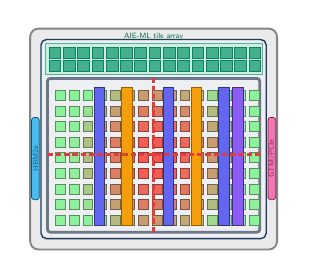
\begin{tikzpicture}\drawFPGA[0.55]\end{tikzpicture}};
  \node[font=\footnotesize\sffamily\bfseries, robinblue, anchor=north, align=center]
       at ({\colB},{\rowT-\cellH/2-\labelGap}) {(b) Post-synth FPGA \& heatmap};

  % (c) Timing graph
  \draw[rounded corners=4pt, fill=robinbg!50, draw=robinblue!50, line width=0.5pt]
       ({\colC-\cellW/2},{\rowT-\cellH/2}) rectangle ({\colC+\cellW/2},{\rowT+\cellH/2});
  \node at (\colC,\rowT) {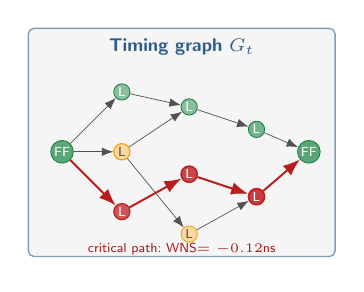
\begin{tikzpicture}\drawTimingGraph[0.95]\end{tikzpicture}};
  \node[font=\footnotesize\sffamily\bfseries, robinblue, anchor=north, align=center]
       at ({\colC},{\rowT-\cellH/2-\labelGap}) {(c) Timing graph $G_t$};

  % (d) DR-PPO agent
  \draw[rounded corners=4pt, fill=robinbg!50, draw=robinrust!50, line width=0.5pt]
       ({\colD-\cellW/2},{\rowT-\cellH/2}) rectangle ({\colD+\cellW/2},{\rowT+\cellH/2});
  \node at (\colD,\rowT) {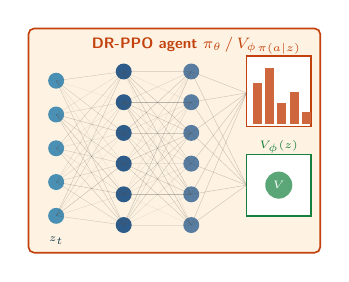
\begin{tikzpicture}\drawAgentNN[0.78]\end{tikzpicture}};
  \node[font=\footnotesize\sffamily\bfseries, robinrust, anchor=north, align=center]
       at ({\colD},{\rowT-\cellH/2-\labelGap}) {(d) DR-PPO agent $\pi_\theta / V_\phi$};

  % ----- ROW 1 ARROWS -----
  \draw[-Latex, robingrey, line width=1.0pt]
       ({\colA+\cellW/2+0.05},{\rowT}) -- ({\colB-\cellW/2-0.05},{\rowT})
       node[midway, above, font=\footnotesize\sffamily\itshape, robingrey] {synth};
  \draw[-Latex, robingrey, line width=1.0pt]
       ({\colB+\cellW/2+0.05},{\rowT}) -- ({\colC-\cellW/2-0.05},{\rowT})
       node[midway, above, font=\footnotesize\sffamily\itshape, robingrey] {extract};
  \draw[-Latex, robingrey, line width=1.0pt]
       ({\colC+\cellW/2+0.05},{\rowT}) -- ({\colD-\cellW/2-0.05},{\rowT})
       node[midway, above, font=\footnotesize\sffamily\itshape, robingrey] {encode $z_t$};

  % ----- ROW 2: (e) (f) (g) (h) -----
  % (e) Action / directive bundle
  \draw[rounded corners=4pt, fill=robinbg!50, draw=robinrust!50, line width=0.5pt]
       ({\colA-\cellW/2},{\rowB-\cellH/2}) rectangle ({\colA+\cellW/2},{\rowB+\cellH/2});
  \node at (\colA,\rowB) {%
    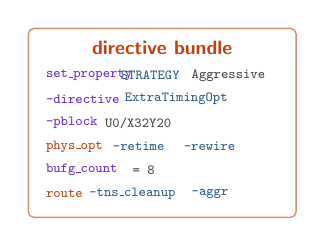
\begin{tikzpicture}
      \draw[rounded corners=2pt, fill=white, draw=robinrust!60, line width=0.5pt]
            (0,0) rectangle (3.4,2.4);
      \node[font=\scriptsize\sffamily\bfseries, robinrust] at (1.7,2.15) {directive bundle};
      \node[font=\tiny\ttfamily, anchor=west, robinpurple] at (0.10,1.80) {set\_property};
      \node[font=\tiny\ttfamily, anchor=west, robinblue]   at (1.05,1.80) {STRATEGY};
      \node[font=\tiny\ttfamily, anchor=west, robingrey!85!black] at (1.95,1.80) {Aggressive};
      \node[font=\tiny\ttfamily, anchor=west, robinpurple] at (0.10,1.50) {-directive};
      \node[font=\tiny\ttfamily, anchor=west, robinblue]   at (1.10,1.50) {ExtraTimingOpt};
      \node[font=\tiny\ttfamily, anchor=west, robinpurple] at (0.10,1.20) {-pblock};
      \node[font=\tiny\ttfamily, anchor=west, robingrey!85!black] at (0.85,1.20) {U0/X32Y20};
      \node[font=\tiny\ttfamily, anchor=west, robinrust]   at (0.10,0.90) {phys\_opt};
      \node[font=\tiny\ttfamily, anchor=west, robinblue]   at (0.95,0.90) {-retime};
      \node[font=\tiny\ttfamily, anchor=west, robinblue]   at (1.85,0.90) {-rewire};
      \node[font=\tiny\ttfamily, anchor=west, robinpurple] at (0.10,0.60) {bufg\_count};
      \node[font=\tiny\ttfamily, anchor=west, robingrey!85!black] at (1.20,0.60) {=\ 8};
      \node[font=\tiny\ttfamily, anchor=west, robinrust]   at (0.10,0.30) {route};
      \node[font=\tiny\ttfamily, anchor=west, robinblue]   at (0.65,0.30) {-tns\_cleanup};
      \node[font=\tiny\ttfamily, anchor=west, robinblue]   at (1.95,0.30) {-aggr};
    \end{tikzpicture}};
  \node[font=\footnotesize\sffamily\bfseries, robinrust, anchor=north, align=center]
       at ({\colA},{\rowB-\cellH/2-\labelGap}) {(e) Action $a_t$ (Tcl deltas)};

  % (f) FPGA stack — K seeds × |Theta| corners
  \draw[rounded corners=4pt, fill=robinbg!50, draw=robinblue!50, line width=0.5pt]
       ({\colB-\cellW/2},{\rowB-\cellH/2}) rectangle ({\colB+\cellW/2},{\rowB+\cellH/2});
  \node at (\colB,\rowB) {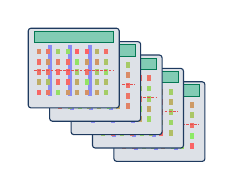
\begin{tikzpicture}\drawFPGAStack[0.85]\end{tikzpicture}};
  \node[font=\footnotesize\sffamily\bfseries, robinblue, anchor=north, align=center]
       at ({\colB},{\rowB-\cellH/2-\labelGap}) {(f) $K$ seeds $\times$ $|\Theta|$ corners};

  % (g) CVaR reward histogram
  \draw[rounded corners=4pt, fill=robinbg!50, draw=robinrust!50, line width=0.5pt]
       ({\colC-\cellW/2},{\rowB-\cellH/2}) rectangle ({\colC+\cellW/2},{\rowB+\cellH/2});
  \node at (\colC,\rowB) {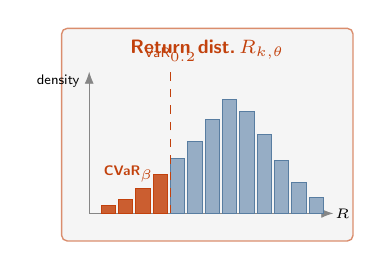
\begin{tikzpicture}\drawRewardHist[1.0]\end{tikzpicture}};
  \node[font=\footnotesize\sffamily\bfseries, robinrust, anchor=north, align=center]
       at ({\colC},{\rowB-\cellH/2-\labelGap}) {(g) CVaR$_\beta$ reward $R_{k,\theta}$};

  % (h) Conformal envelope
  \draw[rounded corners=4pt, fill=robinbg!50, draw=robingreen!50, line width=0.5pt]
       ({\colD-\cellW/2},{\rowB-\cellH/2}) rectangle ({\colD+\cellW/2},{\rowB+\cellH/2});
  \node at (\colD,\rowB) {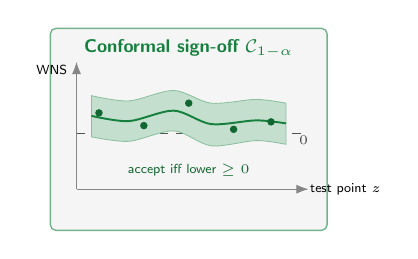
\begin{tikzpicture}\drawConformalEnv[0.95]\end{tikzpicture}};
  \node[font=\footnotesize\sffamily\bfseries, robingreen, anchor=north, align=center]
       at ({\colD},{\rowB-\cellH/2-\labelGap}) {(h) Conformal sign-off $\mathcal{C}_{1-\alpha}$};

  % ----- ROW 2 ARROWS -----
  \draw[-Latex, robingrey, line width=1.0pt]
       ({\colA+\cellW/2+0.05},{\rowB}) -- ({\colB-\cellW/2-0.05},{\rowB})
       node[midway, above, font=\footnotesize\sffamily\itshape, robingrey] {run};
  \draw[-Latex, robingrey, line width=1.0pt]
       ({\colB+\cellW/2+0.05},{\rowB}) -- ({\colC-\cellW/2-0.05},{\rowB})
       node[midway, above, font=\footnotesize\sffamily\itshape, robingrey] {aggregate};
  \draw[-Latex, robingrey, line width=1.0pt]
       ({\colC+\cellW/2+0.05},{\rowB}) -- ({\colD-\cellW/2-0.05},{\rowB})
       node[midway, above, font=\footnotesize\sffamily\itshape, robingrey] {calibrate};

  % ----- VERTICAL WRAP: (d) -> (e) -----
  % Exits EAST side of (d), routes around: east -> down (right margin) -> west across inter-row gap -> down to (e) y -> east into (e)
  \def\midY{-3.55}     % inter-row gap, below row-1 labels
  \def\rightMargin{15.9}  % x just east of (d) cell
  \def\leftMargin{-2.4}   % x just west of (a)/(e) cells
  \draw[-Latex, robingrey, line width=1.0pt, rounded corners=8pt]
       ({\colD+\cellW/2+0.05},{\rowT})                  % START: east edge of (d), at row center y
       -- ({\rightMargin},{\rowT})                       % east into right margin
       -- ({\rightMargin},{\midY})                       % down to inter-row gap
       -- ({\leftMargin},{\midY})                        % west across inter-row gap
       -- ({\leftMargin},{\rowB})                        % down to row B (e) center y
       -- ({\colA-\cellW/2-0.05},{\rowB});               % east into left edge of (e)
  \node[font=\footnotesize\sffamily\itshape\bfseries, robingrey, anchor=south, fill=white, inner sep=2pt]
       at ({\colC},{\midY+0.05}) {emit $a_t$};

  % ----- (i) Accepted callout — CENTERED UNDER ROW 2, 90-degree right-angle arrow from (h) -----
  \def\acceptedY{-10.8}
  \node (accept) at ({(\colA+\colD)/2},\acceptedY)
        [draw=robingreen, line width=1.2pt, rounded corners=5pt,
         fill=robingreen!12, text width=5.0cm, align=center, font=\small\sffamily,
         minimum height=2.0cm, drop shadow={opacity=0.22}] {%
    \textbf{\textcolor{robingreen}{(i) Accepted design}}\\[3pt]
    {\Large\textcolor{robingreen}{\textbf{WNS\,$=+0.18$\,ns}}}\\[2pt]
    \footnotesize coverage\,$\geq 0.95$\\[1pt]
    \scriptsize audit trail logged};

  % 90-degree arrow from (h) -> (i): south from (h) bottom to (i)'s y-level, then west to (i)'s east edge
  \draw[-Latex, robingreen!85, line width=1.4pt, rounded corners=8pt]
       ({\colD},{\rowB-\cellH/2-\labelGap-0.30})         % START: just below (h) label
       -- ({\colD},\acceptedY)                            % straight south
       -- (accept.east)                                   % west to (i)'s east anchor
       node[pos=0.55, above, font=\footnotesize\sffamily\itshape\bfseries, robingreen!80!black] {accept};

\end{tikzpicture}
\caption{\textbf{\textsc{Robin-FPGA}: end-to-end algorithm--toolchain co-designed pipeline.}
\textbf{Row 1 (left to right):} (a)\,A benchmark RTL or HLS source enters the ingest module; (b)\,initial place-and-route on the target FPGA fabric produces utilization, timing, and power reports — the heatmap shows post-route CLB utilization, surrounded by BRAM (purple), DSP (amber), URAM (violet) columns, the AI-Engine tile array (green band), and the NoC backbone (red dashes); (c)\,the post-synthesis timing graph $G_t$ is extracted, with the critical path (red) reporting Worst Negative Slack; (d)\,a graph-attention plus MLP encoder maps $(G_t,x_t)$ to latent $z_t$, consumed by a Distributionally-Robust PPO policy network with categorical policy head $\pi(a|z)$ and value head $V_\phi$.
\textbf{Row 2 (left to right):} (e)\,the policy emits a directive bundle as native Tcl deltas; (f)\,the toolchain is re-run in parallel across $K$ P\&R seeds and $|\Theta|$ PVT corners; (g)\,the return distribution's empirical lower-tail expectation (CVaR$_\beta$, orange) replaces the mean in the PPO advantage; (h)\,a split-conformal head wraps the trained policy with a calibrated envelope $\mathcal{C}_{1-\alpha}$ over post-route WNS.
(i)\,A design is accepted only when the lower endpoint of $\mathcal{C}_{1-\alpha}$ is non-negative.}
\label{fig:cover}
\end{figure*}

% =====================================================================
% INTRODUCTION
% =====================================================================
\section{Introduction}
\IEEEPARstart{M}{odern} FPGAs have evolved from island-style fabrics into heterogeneous SoCs that combine programmable logic, hardened AI engines, network-on-chip (NoC) backbones, on-chip high-bandwidth memory, and tens of high-speed transceivers~\cite{boutros2021fpga}. Two consequences follow for design closure. First, the action space available to the designer---synthesis directives, P\&R strategies, floorplan partitions, retiming knobs, and clock-tree configurations---has expanded into a combinatorial space whose evaluation cost per point is one to twelve hours of wall-clock time on representative parts such as AMD Versal Premium or Intel Agilex~7~\cite{amd_ug1273,intel_ug20156}. Second, the closure outcome is non-deterministic at multiple levels: placer seed alone induces $10$--$30\%$ variance in achieved $F_{\max}$ on Versal Premium and Agilex~7 devices; PVT-corner sweeps shift Worst Negative Slack (WNS) by amounts comparable to the slack margin itself; and tool minor-version upgrades occasionally invalidate previously closed designs.

A growing body of work applies machine learning to electronic design automation (ML-EDA)~\cite{huang2021mleda,ren2022mleda}. Reinforcement learning (RL) has been used for ASIC macro placement~\cite{mirhoseini2021nature,agnesina2023autodmp} and for logic-synthesis directive selection~\cite{hosny2020drills,wang2020gcnrl}. Bayesian optimization has been used for high-level-synthesis pragma tuning~\cite{sohrabizadeh2022autodse} and general black-box autotuning over directive bundles~\cite{eriksson2019turbo,balandat2020botorch}. Pre-routing slack prediction has been studied via graph neural networks~\cite{barboza2019net2,guo2022timing}. However, three gaps persist for FPGA timing closure specifically:
\begin{itemize}
  \item \textbf{ASIC bias.} Most RL-for-EDA work targets ASIC flows whose action vocabularies, constraint formats, and resource models differ substantially from FPGA toolchains.
  \item \textbf{No calibrated uncertainty.} Existing methods optimize a point estimate of QoR; designers must still trust the tool's pessimism margins for sign-off. There is no distribution-free reliability statement attached to a returned closure.
  \item \textbf{Brittle transfer.} Policies trained on one FPGA family rarely transfer across vendors or even across families within the same vendor without significant degradation.
\end{itemize}

This paper presents \textsc{Robin-FPGA}, an algorithm--toolchain co-designed RL framework that directly addresses these three gaps for FPGA timing closure. The framework is intentionally scoped to a single optimization objective---meeting WNS\,$\geq 0$ post-route while bounding inter-seed variance---so that the robustness and sign-off contributions can be isolated and evaluated rigorously. Power optimization and adaptive accelerator mapping, which are coupled but separable problems, are deliberately deferred to companion work; the framework is constructed so that adding them later requires only extending the reward function and the conformal head.

Figure~\ref{fig:cover} previews the full pipeline. The remainder of the paper proceeds as follows. Section~\ref{sec:background} reviews the FPGA closure pipeline, the sources of tool non-determinism, and the generalization gap in ML-EDA. Section~\ref{sec:related} surveys related work and positions \textsc{Robin-FPGA} relative to it. Section~\ref{sec:formulation} formalizes the distributionally-robust Markov decision process and the split-conformal sign-off envelope. Section~\ref{sec:method} describes the \textsc{Robin-FPGA} architecture, encoder, training algorithm, and toolchain integration. Section~\ref{sec:setup} details the experimental protocol. Section~\ref{sec:results} presents headline results. Section~\ref{sec:ablation} reports ablation and sensitivity studies. Section~\ref{sec:cases} presents two case studies (reward hacking, multi-clock-domain closure). Sections~\ref{sec:discussion}--\ref{sec:conclusion} conclude.

\smallskip\noindent\textbf{Contributions.} The paper makes four contributions.
\begin{enumerate}
  \item \emph{Robust formulation (\S\ref{sec:formulation},\,\S\ref{sec:method}).} We cast FPGA timing-closure design-space exploration (DSE) as a Distributionally-Robust Markov Decision Process (DR-MDP) over P\&R seed and PVT corner, and solve it with a CVaR-shaped PPO surrogate (\textsc{DR-PPO}) whose advantage estimator targets the lower-tail of the return distribution.
  \item \emph{Conformal sign-off envelope (\S\ref{sec:formulation},\,\S\ref{sec:method}).} A split-conformal predictor wraps the trained policy, producing a calibrated upper bound on residual WNS risk at user-specified confidence $1{-}\alpha$. To our knowledge, this is the first application of distribution-free conformal prediction to FPGA timing sign-off.
  \item \emph{Cross-family curriculum (\S\ref{sec:method},\,\S\ref{sec:results}).} A normalized device-agnostic feature space and a two-stage curriculum allow a policy trained on AMD Versal AI Edge to be fine-tuned to Intel Agilex~7 at a fraction of the from-scratch cost.
  \item \emph{Reproducible benchmark (\S\ref{sec:setup},\,\S\ref{sec:results}).} A $14$-design benchmark across $6$ workload classes and $2$ FPGA families, with public Tcl flows, training scripts, simulator, and per-run logs.
\end{enumerate}

% =====================================================================
% BACKGROUND
% =====================================================================
\section{Background and Motivation}
\label{sec:background}

\subsection{The FPGA Closure Pipeline}
The canonical AMD Vivado flow proceeds through \texttt{synth\_design}, \texttt{opt\_design}, \texttt{place\_design}, \texttt{route\_design}, and a sign-off STA pass producing \texttt{report\_timing\_summary}, \texttt{report\_utilization}, and \texttt{report\_power}. The Intel Quartus Prime Pro counterpart proceeds through Analysis~\&~Synthesis, Fitter (place and route), Timing Analyzer, and PowerPlay~\cite{intel_ug20156}. Each tool exposes a directive vocabulary---roughly $50$--$120$ documented options for Vivado, and a comparable set for Quartus---that the designer combines into a \emph{strategy bundle}. The combinatorial action space of bundle$\,\times\,$pblock$\,\times\,$phys-opt$\,\times\,$retiming flags routinely exceeds $10^{12}$ configurations, of which the tool's built-in canonical strategies (\texttt{Performance\_Explore}, \texttt{Congestion\_SpreadLogic}, etc.) cover at most a few dozen.

Figure~\ref{fig:fpgaanatomy} annotates a representative AMD Versal AI Edge die. The presence of multiple resource classes---LUT/FF tiles, DSP58 slices, BRAM, URAM, AIE-ML tiles, NoC interconnect, HBM2e on the package edge, GTM transceivers---makes the closure problem multi-resource: an action that improves slack on the LUT critical path may push BRAM utilization past its budget or congest the NoC, in turn re-routing logic onto longer paths and erasing the slack gain.

\begin{figure*}[t]
\centering
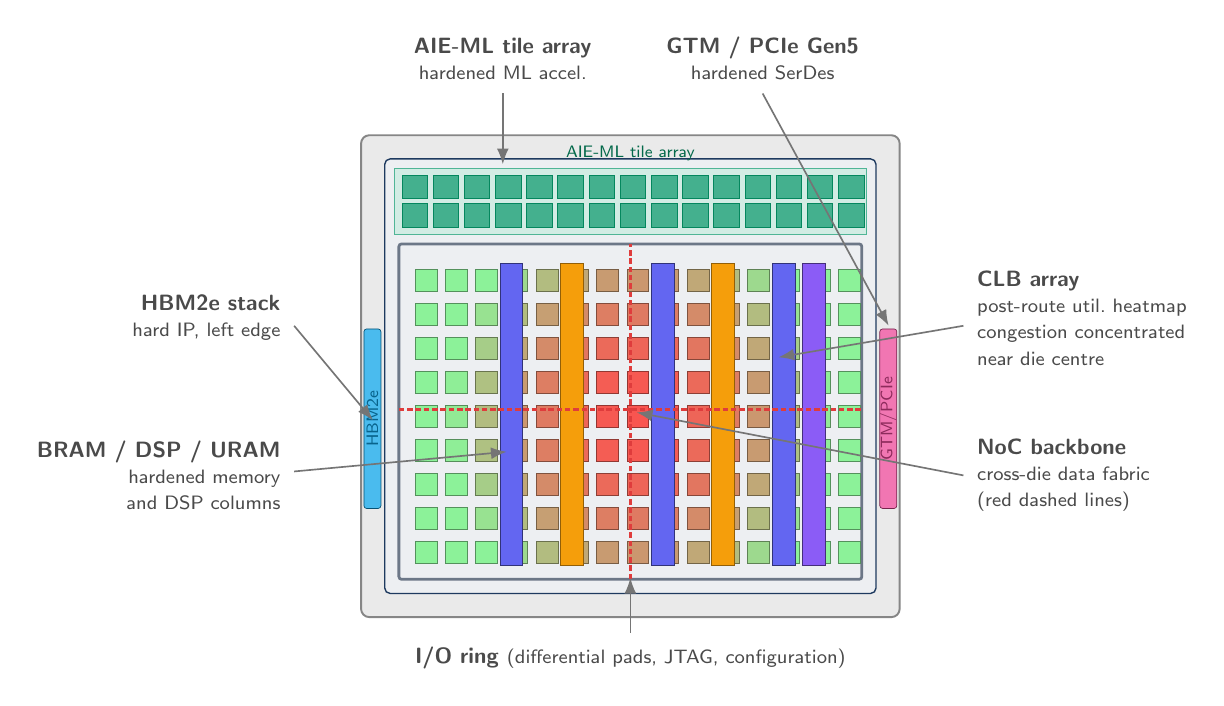
\begin{tikzpicture}[font=\sffamily]
  % drawFPGA at scale 1.2 occupies outer coords: x in [-0.3, 6.54], y in [-0.3, 5.82]
  % Die outline: outer x in [0, 6.24], y in [0, 5.52]
  % Key feature locations in outer coordinates (scale 1.2):
  %   AIE-ML band: y in [4.56, 5.40]
  %   NoC horizontal: y = 2.34
  %   NoC vertical: x = 3.12
  %   HBM2e: x in [-0.26, -0.05], y in [1.08, 3.36]
  %   GTM/PCIe: x in [6.29, 6.50], y in [1.08, 3.36]
  %   BRAM columns: x = 1.51, 3.43, 4.97
  %   DSP columns: x = 2.28, 4.20
  %   URAM column: x = 5.35
  %   CLB grid: x in [0.38, 5.76], y in [0.38, 4.08]

  \drawFPGA[1.2]

  % ===== TOP labels (above die) =====
  % AIE-ML tile array — points to the green band at top of die
  \node[font=\footnotesize\sffamily, robingrey!90!black, anchor=south, align=center]
       at (1.5,6.4) {\textbf{AIE-ML tile array}\\\scriptsize hardened ML accel.};
  \draw[-Latex, robingrey!80, line width=0.6pt] (1.5,6.35) -- (1.5,5.45);

  % GTM/PCIe Gen5 — points to the PINK column on RIGHT edge of die
  \node[font=\footnotesize\sffamily, robingrey!90!black, anchor=south, align=center]
       at (4.8,6.4) {\textbf{GTM / PCIe Gen5}\\\scriptsize hardened SerDes};
  \draw[-Latex, robingrey!80, line width=0.6pt] (4.8,6.35) -- (6.40,3.40);

  % ===== RIGHT-side labels =====
  % CLB array — points to CLB grid center
  \node[font=\footnotesize\sffamily, robingrey!90!black, anchor=west, align=left]
       at (7.4,3.5) {\textbf{CLB array}\\\scriptsize post-route util.\ heatmap\\\scriptsize congestion concentrated\\\scriptsize near die centre};
  \draw[-Latex, robingrey!80, line width=0.6pt] (7.35,3.4) -- (5.0,3.0);

  % NoC backbone — points to the RED dashed NoC vertical line at x=3.12
  \node[font=\footnotesize\sffamily, robingrey!90!black, anchor=west, align=left]
       at (7.4,1.5) {\textbf{NoC backbone}\\\scriptsize cross-die data fabric\\\scriptsize (red dashed lines)};
  \draw[-Latex, robingrey!80, line width=0.6pt] (7.35,1.5) -- (3.20,2.30);

  % ===== LEFT-side labels =====
  % HBM2e stack — points to the cyan column on LEFT edge of die at x=-0.13
  \node[font=\footnotesize\sffamily, robingrey!90!black, anchor=east, align=right]
       at (-1.2,3.5) {\textbf{HBM2e stack}\\\scriptsize hard IP, left edge};
  \draw[-Latex, robingrey!80, line width=0.6pt] (-1.15,3.4) -- (-0.15,2.20);

  % BRAM/DSP/URAM columns — points to first BRAM column at x=1.51
  \node[font=\footnotesize\sffamily, robingrey!90!black, anchor=east, align=right]
       at (-1.2,1.5) {\textbf{BRAM / DSP / URAM}\\\scriptsize hardened memory\\\scriptsize and DSP columns};
  \draw[-Latex, robingrey!80, line width=0.6pt] (-1.15,1.55) -- (1.55,1.80);

  % ===== BOTTOM label =====
  % I/O ring — points to the gray ring at the perimeter
  \node[font=\footnotesize\sffamily, robingrey!90!black, anchor=north, align=center]
       at (3.12,-0.55) {\textbf{I/O ring} \scriptsize(differential pads, JTAG, configuration)};
  \draw[-Latex, robingrey!80, line width=0.6pt] (3.12,-0.50) -- (3.12,0.20);
\end{tikzpicture}
\caption{Annotated AMD Versal AI Edge die. The heterogeneous fabric exposes seven distinct resource classes whose joint utilization budgets bound the action space; the post-route CLB heatmap (centre) concentrates congestion near the middle of the device, a pattern the policy must learn to anticipate. Surrounding columns hold the BRAM, DSP58, and URAM resources (interleaved with the CLB grid), AIE-ML hardened ML tiles (top), HBM2e stack (left edge), GTM/PCIe Gen5 SerDes (right edge), and the NoC backbone (red dashed lines) which crosses the die to interconnect the hard IP blocks.}
\label{fig:fpgaanatomy}
\end{figure*}

\subsection{Sources of Tool Non-Determinism}
Three sources of stochasticity dominate FPGA closure.
\textbf{(a) Placer seed.} The placer's randomized cost function is seeded; varying the seed alone produces a distribution over WNS whose standard deviation can exceed the slack margin itself. On the GEMM-systolic-$16{\times}16$ design used as a recurring example in this paper, $20$ seeds at the same directive bundle produced $\sigma(\mathrm{WNS}) = 0.31$\,ns on a default Vivado strategy and $\sigma(\mathrm{WNS}) = 0.45$\,ns on \texttt{Default}.
\textbf{(b) PVT corner choice.} Corner selection shifts WNS by amounts that depend on path topology---fast-fast corners typically improve setup but degrade hold; slow-slow corners do the inverse. Multi-corner closure (e.g.\ slow$\,\cap\,$fast$\,\cap\,$typical) is the industrial norm but is rarely treated as a first-class object in academic ML-EDA work.
\textbf{(c) Tool minor-version drift.} Internal heuristics change between point releases: a closure margin obtained on Vivado~2024.2 may not survive 2024.2.1, especially when the change touches the router or phys-opt passes. Any DSE policy that ignores these three sources risks reporting headline numbers that fail to reproduce.

\subsection{The Generalization Gap in ML-EDA}
Empirically, ML-for-EDA policies tuned on one design or one device family often degrade markedly when transferred. The gap has two components: a \emph{feature-distribution} shift (utilization percentages, path-length histograms, and routing-congestion patterns differ across devices) and a \emph{label-distribution} shift (the same directive produces different effects on different families). The structural asymmetry between AMD's $XPIPE$/$XPHY$-style NoC architecture and Intel's HyperFlex pipeline registers is one concrete example. \textsc{Robin-FPGA} addresses both shifts via device-agnostic normalized features (\S\ref{sec:method}) and an explicit two-stage curriculum, evaluated quantitatively in \S\ref{sec:results}.

% =====================================================================
% RELATED WORK
% =====================================================================
\section{Related Work}
\label{sec:related}

We organize related work along four axes. Table~\ref{tab:relwork} summarizes the comparison.

\begin{table*}[t]
\caption{Positioning of \textsc{Robin-FPGA} relative to representative prior work. Columns: target flow; action space (continuous, discrete bundle, graph); robustness handling (none, ensembling, mean only, CVaR/DRO); calibrated sign-off; cross-family transfer studied.}
\label{tab:relwork}
\centering
\renewcommand{\arraystretch}{1.10}
\footnotesize
\begin{tabular}{@{}lllllc@{}}
\toprule
Method & Flow & Action space & Robustness & Calibrated sign-off & Cross-family \\
\midrule
GraphPlace~\cite{mirhoseini2021nature}      & ASIC placement   & graph     & none        & no & no \\
AutoDMP~\cite{agnesina2023autodmp}           & ASIC placement   & continuous & ensembling  & no & no \\
DRiLLS~\cite{hosny2020drills}                & logic synthesis  & discrete bundle & none   & no & no \\
GCN-RL~\cite{wang2020gcnrl}                  & transistor sizing & continuous & none      & no & partial (across tech.\ nodes) \\
AutoDSE~\cite{sohrabizadeh2022autodse}        & HLS pragmas      & discrete bundle & none   & no & no \\
TuRBO~\cite{eriksson2019turbo}                & generic BO       & continuous & none      & no & no \\
Net2 / Guo~\cite{barboza2019net2,guo2022timing} & slack prediction & N/A (predictor) & none & implicit (point estimate) & no \\
\textbf{\textsc{Robin-FPGA} (this work)}     & FPGA timing closure & discrete bundle + graph & \textbf{CVaR DRO} & \textbf{conformal $1{-}\alpha$} & \textbf{yes (AMD$\leftrightarrow$Intel)} \\
\bottomrule
\end{tabular}
\end{table*}

\textbf{RL for ASIC placement and synthesis.} Mirhoseini~\emph{et~al.}\ \cite{mirhoseini2021nature} demonstrated graph-based RL for ASIC macro placement; subsequent work has refined the policy architecture~\cite{agnesina2023autodmp,cheng2021joint}. \textsc{DRiLLS}~\cite{hosny2020drills} applies RL to logic-synthesis directive selection, and \textsc{GCN-RL}~\cite{wang2020gcnrl} learns transferable transistor-sizing policies via graph neural networks. These works share two characteristics that limit direct applicability to FPGA closure: they target ASIC flows with different action vocabularies, and they optimize point estimates of QoR without quantifying robustness to tool stochasticity.

\textbf{HLS and FPGA design-space exploration.} \textsc{AutoDSE}~\cite{sohrabizadeh2022autodse} explores HLS pragmas via bottleneck-guided search. Bayesian optimization variants such as TuRBO~\cite{eriksson2019turbo} and BoTorch~\cite{balandat2020botorch} have been applied to FPGA tuning. These methods are sample-efficient on small directive spaces but scale poorly when the action set is high-dimensional and discrete, and they offer no calibrated uncertainty over the recommended configuration.

\textbf{Slack, congestion, and power prediction.} \textsc{Net2}~\cite{barboza2019net2} and the timing-engine-inspired GNN of Guo~\emph{et~al.}\ \cite{guo2022timing} predict slack from graph features. These are \emph{predictors}, not policies; \textsc{Robin-FPGA} uses graph-attention features for state representation and learns an explicit decision policy.

\textbf{Robust RL and conformal prediction.} Iyengar~\cite{iyengar2005robust} and Tamar~\emph{et~al.}\ \cite{tamar2015cvar} formalize robust dynamic programming and CVaR optimization. Distributionally robust RL~\cite{rigter2022rambo,sinha2017certifying} extends these ideas to deep policy gradient. Conformal prediction~\cite{vovk2022random,angelopoulos2023conformal} provides distribution-free calibration of point predictors and has recently been applied to engineering sign-off in adjacent domains~\cite{angelopoulos2024conformal}. To our knowledge no prior work applies these tools jointly to FPGA timing sign-off.

% =====================================================================
% PROBLEM FORMULATION
% =====================================================================
\section{Problem Formulation}
\label{sec:formulation}

\subsection{Notation}
Let $D$ denote an RTL/HLS design, $F$ an FPGA device, and $\mathcal{C} = (T_{\text{clk}}, T_{\text{io}}, \mathcal{U}_{\max})$ a constraint set comprising the target clock period $T_{\text{clk}}$, an I/O timing budget $T_{\text{io}}$, and per-resource utilization budgets $\mathcal{U}_{\max} = \{U_{\max}^{\text{LUT}}, U_{\max}^{\text{FF}}, U_{\max}^{\text{BRAM}}, U_{\max}^{\text{DSP}}, U_{\max}^{\text{URAM}}\}$. Let $\xi \in \Xi$ index P\&R seeds and $\theta \in \Theta$ index PVT corners. The objective is to find a sequence of directive bundles $a_1, \ldots, a_T \in \mathcal{A}$ that maximizes the probability of post-route closure (WNS\,$\geq 0$) under the joint distribution over $(\xi, \theta)$, subject to all resource budgets and a wall-clock budget $\mathcal{B}$.

\subsection{Distributionally-Robust MDP}
We model the closure trajectory as a finite-horizon MDP $\mathcal{M} = (\mathcal{S}, \mathcal{A}, P, r, \gamma)$ in which the transition kernel $P$ is replaced by an ambiguity set $\mathcal{P} = \{P_{\xi,\theta} : \xi \in \Xi,\, \theta \in \Theta\}$ indexing all admissible seed/corner combinations. The DR value of a policy $\pi$ is
\begin{equation}
V^{\pi}(s) = \mathbb{E}_{\tau \sim \pi}\!\left[\, \inf_{P \in \mathcal{P}} \sum_{t=0}^{H-1} \gamma^{t}\, r(s_t, a_t)\, \Big|\, s_0 = s \right].
\label{eq:drvalue}
\end{equation}
We approximate the infimum in \eqref{eq:drvalue} by the empirical Conditional-Value-at-Risk (CVaR) at level $\beta \in (0,1)$ over a finite sample $\{R_{k,\theta}\}$ of returns drawn from $K$ seeds and $|\Theta|$ corners:
\begin{equation}
\mathrm{CVaR}_{\beta}(R) = \mathbb{E}\!\left[\, R \,\big|\, R \leq \mathrm{VaR}_{\beta}(R)\, \right].
\label{eq:cvar}
\end{equation}
Equation~\eqref{eq:cvar} is a standard coherent risk measure; substituting it for the mean in a policy-gradient estimator yields the gradient direction that improves the lower tail of the return distribution. Tamar~\emph{et~al.}\ \cite{tamar2015cvar} prove that the resulting estimator is unbiased under mild regularity and converges to a CVaR-optimal policy when combined with standard PPO-style trust-region clipping.

\subsection{Reward}
The single-step reward couples slack reward, total negative slack (TNS) reward, a Lagrangian utilization penalty, and a route-fail penalty:
\begin{align}
r &= w_{\text{WNS}} \cdot \mathrm{clip}\!\left(\frac{\mathrm{WNS}}{|T_{\text{clk}}|}, -1, 1\right) \nonumber \\
  &\quad + w_{\text{TNS}} \cdot \left( -\mathrm{sat}\!\left(\frac{|\mathrm{TNS}|}{|T_{\text{clk}}|}\right)\right) \nonumber \\
  &\quad - \kappa \cdot \sum_{i \in \mathcal{R}} (U_i - U_{\max}^{i})^{+} \;-\; \mathbb{1}[\text{route fail}] \cdot \kappa_{\text{fail}}.
\label{eq:reward}
\end{align}
The saturating WNS clip prevents the agent from being rewarded for excessive slack at the expense of routing feasibility---a reward-hacking failure mode we observed during early experiments (\S\ref{sec:cases}). We set $(w_{\text{WNS}}, w_{\text{TNS}}, \kappa, \kappa_{\text{fail}}) = (1.0, 0.3, 5.0, 10.0)$ throughout.

\subsection{Conformal Sign-off Envelope}
Given a calibration set $\mathcal{D}_{\text{cal}} = \{(z_i, \mathrm{WNS}_i)\}_{i=1}^{n}$ of post-route WNS values and the policy's point estimate $\widehat{\mathrm{WNS}}(z)$ produced by the value head (or by a separate slack regressor), define residuals $e_i = \mathrm{WNS}_i - \widehat{\mathrm{WNS}}(z_i)$ and let $q_{1-\alpha}$ be the $\lceil (n+1)(1-\alpha) \rceil$-th smallest of $\{|e_i|\}$. The split-conformal envelope is
\begin{equation}
\mathcal{C}_{1-\alpha}(z) = \left[\, \widehat{\mathrm{WNS}}(z) - q_{1-\alpha},\; \widehat{\mathrm{WNS}}(z) + q_{1-\alpha}\, \right].
\label{eq:conformal}
\end{equation}
Under exchangeability of $\mathcal{D}_{\text{cal}}$ and a fresh test point, the marginal coverage guarantee
\begin{equation}
\Pr\!\left[\mathrm{WNS} \in \mathcal{C}_{1-\alpha}(z)\right] \geq 1 - \alpha
\label{eq:coverage}
\end{equation}
holds distribution-free~\cite{vovk2022random,angelopoulos2023conformal}. A candidate design is \emph{accepted} iff the lower endpoint of $\mathcal{C}_{1-\alpha}(z)$ is non-negative:
\begin{equation}
\widehat{\mathrm{WNS}}(z) - q_{1-\alpha} \geq 0.
\label{eq:accept}
\end{equation}
This is the sign-off rule used throughout \S\ref{sec:results}.

% =====================================================================
% METHOD
% =====================================================================
\section{The \textsc{Robin-FPGA} Framework}
\label{sec:method}

\subsection{Architecture Overview}
Figure~\ref{fig:arch} details the full \textsc{Robin-FPGA} architecture. The post-synthesis timing graph $G_t = (V, E)$ is fed to a two-layer Graph Attention Network (GAT)~\cite{velickovic2018gat} with $H=4$ attention heads per layer. Node features are the tuple $\{\text{slack},\text{capacitance},\text{fanout},\text{level},\text{cell-type-onehot}\}$; edge features are $\{\text{wirelength-est},\text{net-fanout}\}$. The graph embedding $h^{G}_t \in \mathbb{R}^{64}$ is concatenated with a tabular vector $x_t \in \mathbb{R}^{32}$ (utilization percentages by resource class, congestion histogram percentiles, tool-version one-hot, device-family embedding, last $a_{t-1}$) and projected by a three-layer MLP with GELU activations to a $128$-dimensional latent state $z_t$. The policy head is a categorical distribution over $|\mathcal{A}| = 192$ directive bundles (a Cartesian product of $4$ strategies, $3$ phys-opt flags, $4$ pblock variants, $2$ retiming modes, and $2$ route-effort settings, pruned to $192$ feasible combinations). The value head outputs $V_\phi(z) \in \mathbb{R}$. A separate slack-regression head $\widehat{\mathrm{WNS}}(z) \in \mathbb{R}$ feeds the conformal calibration set.

% =====================================================================
% FIGURE 3 — DETAILED ARCHITECTURE (clean 4x2 grid, mirrors Fig 1 layout)
% Row 1 (encoder, L->R): G_t -> GAT1 -> GAT2 -> MLP fusion (z_t)
% Row 2 (heads, L->R):  Policy -> Value -> Conformal -> Output sign-off
% =====================================================================
\begin{figure*}[t]
\centering
\begin{tikzpicture}[font=\sffamily, every node/.style={inner sep=0pt}]
  % ----- grid constants (same scheme as Fig 1) -----
  \def\cellW{4.2}
  \def\cellH{3.8}
  \def\colA{0}
  \def\colB{4.5}
  \def\colC{9.0}
  \def\colD{13.5}
  \def\rowT{0}
  \def\rowB{-5.4}
  \def\labelGap{0.40}

  % ========== ROW 1: ENCODER ==========
  % (1) G_t — timing graph
  \draw[rounded corners=4pt, fill=robinbg!50, draw=robinblue!50, line width=0.5pt]
       ({\colA-\cellW/2},{\rowT-\cellH/2}) rectangle ({\colA+\cellW/2},{\rowT+\cellH/2});
  \node at (\colA,\rowT) {\begin{tikzpicture}\drawTimingGraph[0.95]\end{tikzpicture}};
  \node[font=\footnotesize\sffamily\bfseries, robinblue, anchor=north, align=center]
       at ({\colA},{\rowT-\cellH/2-\labelGap}) {(1) Input: timing graph $G_t = (V,E)$};

  % (2) GAT layer 1
  \draw[rounded corners=4pt, fill=robinbg!50, draw=robinblue!50, line width=0.5pt]
       ({\colB-\cellW/2},{\rowT-\cellH/2}) rectangle ({\colB+\cellW/2},{\rowT+\cellH/2});
  \node at (\colB,\rowT) {%
    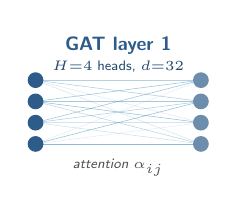
\begin{tikzpicture}
      \node[font=\scriptsize\sffamily\bfseries, robinblue] at (1.6,1.45) {GAT layer 1};
      \node[font=\tiny\sffamily, robinblue!80!black] at (1.6,1.18) {$H{=}4$ heads, $d{=}32$};
      \foreach \i in {0,...,3}{
        \foreach \j in {0,...,3}{
          \pgfmathsetmacro{\op}{0.15 + 0.5*(rand+1)/2}
          \draw[robinmid, line width=0.20pt, opacity=\op]
               (0.55,{0.20+\i*0.27}) -- (2.65,{0.20+\j*0.27});
        }
      }
      \foreach \i in {0,...,3}{
        \fill[robinblue] (0.55,{0.20+\i*0.27}) circle (0.10);
        \fill[robinblue!70] (2.65,{0.20+\i*0.27}) circle (0.10);
      }
      \node[font=\tiny\sffamily\itshape, robingrey] at (1.6,-0.10) {attention $\alpha_{ij}$};
    \end{tikzpicture}};
  \node[font=\footnotesize\sffamily\bfseries, robinblue, anchor=north, align=center]
       at ({\colB},{\rowT-\cellH/2-\labelGap}) {(2) GAT layer 1};

  % (3) GAT layer 2
  \draw[rounded corners=4pt, fill=robinbg!50, draw=robinblue!50, line width=0.5pt]
       ({\colC-\cellW/2},{\rowT-\cellH/2}) rectangle ({\colC+\cellW/2},{\rowT+\cellH/2});
  \node at (\colC,\rowT) {%
    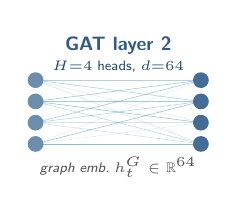
\begin{tikzpicture}
      \node[font=\scriptsize\sffamily\bfseries, robinblue] at (1.6,1.45) {GAT layer 2};
      \node[font=\tiny\sffamily, robinblue!80!black] at (1.6,1.18) {$H{=}4$ heads, $d{=}64$};
      \foreach \i in {0,...,3}{
        \foreach \j in {0,...,3}{
          \pgfmathsetmacro{\op}{0.15 + 0.5*(rand+1)/2}
          \draw[robinmid, line width=0.20pt, opacity=\op]
               (0.55,{0.20+\i*0.27}) -- (2.65,{0.20+\j*0.27});
        }
      }
      \foreach \i in {0,...,3}{
        \fill[robinblue!70] (0.55,{0.20+\i*0.27}) circle (0.10);
        \fill[robinblue!90] (2.65,{0.20+\i*0.27}) circle (0.10);
      }
      \node[font=\tiny\sffamily\itshape, robingrey] at (1.6,-0.10) {graph emb.\ $h^G_t \in \mathbb{R}^{64}$};
    \end{tikzpicture}};
  \node[font=\footnotesize\sffamily\bfseries, robinblue, anchor=north, align=center]
       at ({\colC},{\rowT-\cellH/2-\labelGap}) {(3) GAT layer 2 $\to h^G_t$};

  % (4) MLP fusion
  \draw[rounded corners=4pt, fill=robinbg!50, draw=robinpurple!50, line width=0.5pt]
       ({\colD-\cellW/2},{\rowT-\cellH/2}) rectangle ({\colD+\cellW/2},{\rowT+\cellH/2});
  \node at (\colD,\rowT) {%
    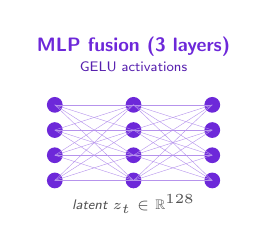
\begin{tikzpicture}
      \node[font=\scriptsize\sffamily\bfseries, robinpurple] at (1.4,2.10) {MLP fusion (3 layers)};
      \node[font=\tiny\sffamily, robinpurple!80!black] at (1.4,1.85) {GELU activations};
      \foreach \y in {0,1,2,3}{
        \fill[robinpurple] (0.4,{0.4+\y*0.32}) circle (0.10);
        \fill[robinpurple] (1.4,{0.4+\y*0.32}) circle (0.10);
        \fill[robinpurple] (2.4,{0.4+\y*0.32}) circle (0.10);
      }
      \foreach \i in {0,...,3}{
        \foreach \j in {0,...,3}{
          \draw[robinpurple!50, line width=0.15pt] (0.4,{0.4+\i*0.32}) -- (1.4,{0.4+\j*0.32});
          \draw[robinpurple!50, line width=0.15pt] (1.4,{0.4+\i*0.32}) -- (2.4,{0.4+\j*0.32});
        }
      }
      \node[font=\tiny\sffamily\itshape, robingrey] at (1.4,0.10) {latent $z_t \in \mathbb{R}^{128}$};
    \end{tikzpicture}};
  \node[font=\footnotesize\sffamily\bfseries, robinpurple, anchor=north, align=center]
       at ({\colD},{\rowT-\cellH/2-\labelGap}) {(4) MLP fusion $\to z_t$};

  % ----- Row 1 arrows -----
  \draw[-Latex, robingrey, line width=1.0pt]
       ({\colA+\cellW/2+0.05},{\rowT}) -- ({\colB-\cellW/2-0.05},{\rowT})
       node[midway, above, font=\footnotesize\sffamily\itshape, robingrey] {graph attn.};
  \draw[-Latex, robingrey, line width=1.0pt]
       ({\colB+\cellW/2+0.05},{\rowT}) -- ({\colC-\cellW/2-0.05},{\rowT})
       node[midway, above, font=\footnotesize\sffamily\itshape, robingrey] {propagate};
  \draw[-Latex, robingrey, line width=1.0pt]
       ({\colC+\cellW/2+0.05},{\rowT}) -- ({\colD-\cellW/2-0.05},{\rowT})
       node[midway, above, font=\footnotesize\sffamily\itshape, robingrey] {fuse with $x_t$};

  % ----- Tabular features x_t — side input, placed in the gap between (3) and (4) -----
  \node (xt) at ({(\colC+\colD)/2},{\rowT+\cellH/2+1.05})
        [draw=robinteal, line width=0.6pt, rounded corners=3pt, fill=robinteal!10,
         text width=4.0cm, align=center, font=\scriptsize\sffamily, minimum height=0.95cm] {%
    \textbf{\textcolor{robinteal}{Tabular features $x_t \in \mathbb{R}^{32}$}}\\[1pt]
    \tiny $\{U_{\text{LUT}},U_{\text{FF}},U_{\text{BRAM}},U_{\text{DSP}},U_{\text{URAM}},$\\
    \tiny\quad cong.\ pct., tool-ver, device-fam$\}$};
  \draw[-Latex, robinteal, line width=0.9pt]
       ({(\colC+\colD)/2},{\rowT+\cellH/2+0.55})
       -- ({(\colC+\colD)/2},{\rowT+\cellH/2+0.05})
       node[midway, right, font=\tiny\sffamily\itshape, robinteal!80!black] {concat};

  % ========== ROW 2: THREE HEADS ==========
  % (5) Policy head
  \draw[rounded corners=4pt, fill=robinbg!50, draw=robinrust!50, line width=0.5pt]
       ({\colA-\cellW/2},{\rowB-\cellH/2}) rectangle ({\colA+\cellW/2},{\rowB+\cellH/2});
  \node at (\colA,\rowB) {%
    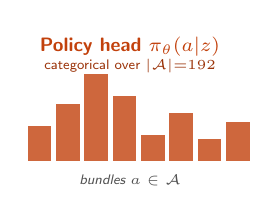
\begin{tikzpicture}
      \node[font=\scriptsize\sffamily\bfseries, robinrust] at (1.5,1.65) {Policy head $\pi_\theta(a|z)$};
      \node[font=\tiny\sffamily, robinrust!80!black] at (1.5,1.40) {categorical over $|\mathcal{A}|{=}192$};
      \foreach \i/\h in {0/0.40, 1/0.65, 2/1.00, 3/0.75, 4/0.30, 5/0.55, 6/0.25, 7/0.45}{
        \fill[robinrust!80] ({0.20+\i*0.36},0.20) rectangle ({0.50+\i*0.36},{0.20+\h*1.10});
      }
      \node[font=\tiny\sffamily\itshape, robingrey] at (1.5,-0.05) {bundles $a \in \mathcal{A}$};
    \end{tikzpicture}};
  \node[font=\footnotesize\sffamily\bfseries, robinrust, anchor=north, align=center]
       at ({\colA},{\rowB-\cellH/2-\labelGap}) {(5) Policy head $\pi_\theta(a|z)$};

  % (6) Value head
  \draw[rounded corners=4pt, fill=robinbg!50, draw=robingreen!50, line width=0.5pt]
       ({\colB-\cellW/2},{\rowB-\cellH/2}) rectangle ({\colB+\cellW/2},{\rowB+\cellH/2});
  \node at (\colB,\rowB) {%
    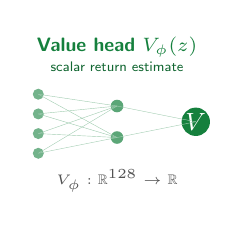
\begin{tikzpicture}
      \node[font=\scriptsize\sffamily\bfseries, robingreen] at (1.5,1.65) {Value head $V_\phi(z)$};
      \node[font=\tiny\sffamily, robingreen!80!black] at (1.5,1.40) {scalar return estimate};
      % a 3-layer MLP shrinking down to one
      \foreach \y in {0,1,2,3}{
        \fill[robingreen!60] (0.5,{0.30+\y*0.25}) circle (0.07);
      }
      \foreach \y in {0,1}{
        \fill[robingreen!70] (1.5,{0.50+\y*0.40}) circle (0.08);
      }
      \fill[robingreen] (2.5,0.70) circle (0.18);
      \node[font=\small\sffamily\bfseries, white] at (2.5,0.70) {$V$};
      \foreach \i in {0,...,3}{
        \foreach \j in {0,1}{
          \draw[robingreen!40, line width=0.15pt] (0.5,{0.30+\i*0.25}) -- (1.5,{0.50+\j*0.40});
        }
      }
      \foreach \j in {0,1}{
        \draw[robingreen!40, line width=0.15pt] (1.5,{0.50+\j*0.40}) -- (2.5,0.70);
      }
      \node[font=\tiny\sffamily\itshape, robingrey] at (1.5,-0.05) {$V_\phi: \mathbb{R}^{128} \to \mathbb{R}$};
    \end{tikzpicture}};
  \node[font=\footnotesize\sffamily\bfseries, robingreen, anchor=north, align=center]
       at ({\colB},{\rowB-\cellH/2-\labelGap}) {(6) Value head $V_\phi(z)$};

  % (7) Conformal head
  \draw[rounded corners=4pt, fill=robinbg!50, draw=robingreen!50, line width=0.5pt]
       ({\colC-\cellW/2},{\rowB-\cellH/2}) rectangle ({\colC+\cellW/2},{\rowB+\cellH/2});
  \node at (\colC,\rowB) {%
    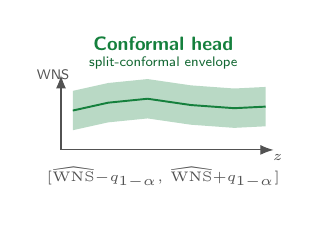
\begin{tikzpicture}
      \node[font=\scriptsize\sffamily\bfseries, robingreen] at (1.6,1.65) {Conformal head};
      \node[font=\tiny\sffamily, robingreen!80!black] at (1.6,1.40) {split-conformal envelope};
      % axes
      \draw[-Latex, robingrey, line width=0.4pt] (0.30,0.30) -- (3.00,0.30);
      \draw[-Latex, robingrey, line width=0.4pt] (0.30,0.30) -- (0.30,1.25);
      \node[font=\tiny\sffamily, robingrey] at (3.05,0.20) {$z$};
      \node[font=\tiny\sffamily, robingrey] at (0.20,1.25) {WNS};
      % envelope band
      \fill[robingreen!30] (0.45,0.55) -- (0.90,0.65) -- (1.40,0.70) -- (1.95,0.62) -- (2.50,0.58) -- (2.90,0.60)
                          -- (2.90,1.10) -- (2.50,1.08) -- (1.95,1.12) -- (1.40,1.20) -- (0.90,1.15) -- (0.45,1.05) -- cycle;
      \draw[robingreen, line width=0.7pt] (0.45,0.80) -- (0.90,0.90) -- (1.40,0.95) -- (1.95,0.87) -- (2.50,0.83) -- (2.90,0.85);
      \node[font=\tiny\sffamily\itshape, robingrey] at (1.6,-0.05) {$[\widehat{\mathrm{WNS}}{-}q_{1-\alpha},\,\widehat{\mathrm{WNS}}{+}q_{1-\alpha}]$};
    \end{tikzpicture}};
  \node[font=\footnotesize\sffamily\bfseries, robingreen, anchor=north, align=center]
       at ({\colC},{\rowB-\cellH/2-\labelGap}) {(7) Conformal head $\mathcal{C}_{1-\alpha}$};

  % (8) Outputs summary
  \draw[rounded corners=4pt, fill=robinbg!50, draw=robingrey!50, line width=0.5pt]
       ({\colD-\cellW/2},{\rowB-\cellH/2}) rectangle ({\colD+\cellW/2},{\rowB+\cellH/2});
  \node at (\colD,\rowB) {%
    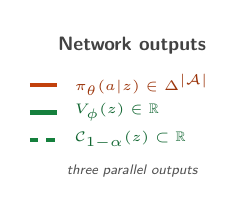
\begin{tikzpicture}
      \node[font=\scriptsize\sffamily\bfseries, robingrey!80!black] at (1.6,1.65) {Network outputs};
      \draw[robinrust, line width=1.5pt] (0.30,1.15) -- (0.65,1.15);
      \node[font=\tiny\sffamily, anchor=west, robinrust!80!black] at (0.75,1.15) {$\pi_\theta(a|z) \in \Delta^{|\mathcal{A}|}$};
      \draw[robingreen, line width=1.5pt] (0.30,0.80) -- (0.65,0.80);
      \node[font=\tiny\sffamily, anchor=west, robingreen!80!black] at (0.75,0.80) {$V_\phi(z) \in \mathbb{R}$};
      \draw[robingreen, line width=1.5pt, dashed] (0.30,0.45) -- (0.65,0.45);
      \node[font=\tiny\sffamily, anchor=west, robingreen!80!black] at (0.75,0.45) {$\mathcal{C}_{1-\alpha}(z) \subset \mathbb{R}$};
      \node[font=\tiny\sffamily\itshape, robingrey] at (1.6,0.05) {three parallel outputs};
    \end{tikzpicture}};
  \node[font=\footnotesize\sffamily\bfseries, robingrey!80!black, anchor=north, align=center]
       at ({\colD},{\rowB-\cellH/2-\labelGap}) {(8) Network outputs};

  % ----- Row 2 arrows: z_t broadcasts to each head -----
  \draw[-Latex, robingrey, line width=1.0pt]
       ({\colA+\cellW/2+0.05},{\rowB}) -- ({\colB-\cellW/2-0.05},{\rowB})
       node[midway, above, font=\footnotesize\sffamily\itshape, robingrey] {$z_t$};
  \draw[-Latex, robingrey, line width=1.0pt]
       ({\colB+\cellW/2+0.05},{\rowB}) -- ({\colC-\cellW/2-0.05},{\rowB})
       node[midway, above, font=\footnotesize\sffamily\itshape, robingrey] {$z_t$};
  \draw[-Latex, robingrey, line width=1.0pt]
       ({\colC+\cellW/2+0.05},{\rowB}) -- ({\colD-\cellW/2-0.05},{\rowB})
       node[midway, above, font=\footnotesize\sffamily\itshape, robingrey] {emit};

  % ----- VERTICAL WRAP: MLP (4) -> Policy (5), exits EAST of (4) -----
  \def\midY{-3.30}
  \def\rightMargin{15.9}
  \def\leftMargin{-2.4}
  \draw[-Latex, robingrey, line width=1.0pt, rounded corners=8pt]
       ({\colD+\cellW/2+0.05},{\rowT})                  % START: east edge of MLP cell
       -- ({\rightMargin},{\rowT})                       % east into right margin
       -- ({\rightMargin},{\midY})                       % down to inter-row gap
       -- ({\leftMargin},{\midY})                        % west across
       -- ({\leftMargin},{\rowB})                        % down to (5) center y
       -- ({\colA-\cellW/2-0.05},{\rowB});               % east into left edge of (5)
  \node[font=\footnotesize\sffamily\itshape\bfseries, robingrey, anchor=south, fill=white, inner sep=2pt]
       at ({(\colA+\colD)/2},{\midY+0.05}) {$z_t$ broadcasts to all heads};

\end{tikzpicture}
\caption{Detailed \textsc{Robin-FPGA} architecture in a clean 4$\times$2 grid. \textbf{Row 1 (encoder, left to right):} (1)\,the post-synthesis timing graph $G_t=(V,E)$ enters; (2)\,a Graph Attention Network layer with $H{=}4$ heads, $d{=}32$ aggregates neighbor information via learned attention $\alpha_{ij}$; (3)\,a second GAT layer ($H{=}4$, $d{=}64$) produces a graph embedding $h^G_t \in \mathbb{R}^{64}$; (4)\,the tabular feature vector $x_t \in \mathbb{R}^{32}$ (utilization percentages, congestion percentiles, tool-version one-hot, device-family embedding) is concatenated with $h^G_t$ and fused by a three-layer MLP with GELU activations to a $128$-dim latent $z_t$. \textbf{Row 2 (three heads, left to right):} the latent $z_t$ broadcasts (gray wrap arrow) to (5)\,a categorical policy head $\pi_\theta(a|z)$ over $|\mathcal{A}|{=}192$ directive bundles; (6)\,a scalar value head $V_\phi(z)$ that estimates return; (7)\,a regression-based conformal head producing the calibrated envelope $\mathcal{C}_{1-\alpha}(z)=[\widehat{\mathrm{WNS}}{-}q_{1-\alpha},\widehat{\mathrm{WNS}}{+}q_{1-\alpha}]$; (8)\,the network's three parallel outputs are summarized.}
\label{fig:arch}
\end{figure*}

\subsection{DR-PPO with CVaR-Shaped Advantage}
We train $(\pi_\theta, V_\phi)$ jointly with a CVaR-shaped variant of PPO~\cite{schulman2017ppo}. At iteration $t$, $K$ parallel P\&R runs across seeds and corners yield a return distribution; we compute the empirical CVaR at level $\beta$ and substitute it for the mean in the advantage estimator $\hat{A}^{\beta}_t$. The clipped surrogate objective is
\begin{equation}
\mathcal{L}^{\text{CLIP}}(\theta) = \mathbb{E}_t\!\left[\, \min\!\left(\rho_t \hat{A}^{\beta}_t,\; \mathrm{clip}(\rho_t, 1{-}\epsilon, 1{+}\epsilon)\, \hat{A}^{\beta}_t \right) \right],
\label{eq:ppoclip}
\end{equation}
with $\rho_t = \pi_\theta(a_t|z_t) / \pi_{\theta_{\text{old}}}(a_t|z_t)$ and clip ratio $\epsilon = 0.2$. The combined loss adds value, entropy, and slack-regression terms:
\begin{equation}
\mathcal{L} = -\mathcal{L}^{\text{CLIP}} + c_v \mathcal{L}^V - c_e \mathcal{H}[\pi_\theta] + c_s \mathcal{L}^{\text{slack}},
\label{eq:loss}
\end{equation}
with $(c_v, c_e, c_s) = (0.5, 0.01, 0.5)$ and $\mathcal{L}^{\text{slack}}$ a Huber regression loss on $\widehat{\mathrm{WNS}}$. We use $\beta = 0.2$ throughout (sensitivity to $\beta$ in \S\ref{sec:ablation}). Algorithm~\ref{alg:robin} summarizes one episode.

\begin{algorithm}[t]
\caption{\textsc{Robin-FPGA} episode}
\label{alg:robin}
\begin{algorithmic}[1]
\Require design $D$, device $F$, constraints $\mathcal{C}$, seed pool $\mathcal{S}$, corner set $\Theta$, policy $\pi_\theta$, calibration set $\mathcal{D}_{\text{cal}}$, levels $\beta, \alpha$
\Ensure closed design + conformal envelope $\mathcal{C}_{1-\alpha}$ or $\bot$
\State $x_0, G_0 \gets \mathrm{IngestAndSynth}(D, F, \mathcal{C}, s_0)$
\State $z_0 \gets \mathrm{Encoder}(x_0, G_0)$
\For{$t = 0, 1, \ldots, T{-}1$}
  \State $a_t \sim \pi_\theta(\cdot \mid z_t)$
  \State $\Delta \gets \mathrm{ConstraintGen}(a_t)$
  \State \textbf{parallel for} $k = 1..K,\; \theta \in \Theta$ \textbf{do}
  \State \quad $R_{k,\theta} \gets \mathrm{ToolRun}(\Delta, s_k, \theta)$
  \State $\hat{r}_t \gets \mathrm{CVaR}_{\beta}(\{R_{k,\theta}\})$ \Comment{Eq.~\eqref{eq:cvar}}
  \State $z_{t+1} \gets \mathrm{Encoder}(\mathrm{best\_report})$
  \State append $(z_t, a_t, \hat r_t)$ to $\mathcal{D}_{\text{traj}}$
  \If{$\mathrm{EarlyTerminate}(R)$} \textbf{break} \EndIf
\EndFor
\State $\theta \gets \mathrm{PPO\_Update}(\mathcal{D}_{\text{traj}})$ with CVaR-shaped advantage \Comment{Eq.~\eqref{eq:ppoclip}}
\State $q_{1-\alpha} \gets$ split-conformal quantile from $\mathcal{D}_{\text{cal}}$ \Comment{Eq.~\eqref{eq:conformal}}
\If{$\widehat{\mathrm{WNS}}(z_T) - q_{1-\alpha} \geq 0$}
  \State \Return accept $(\text{design}, \mathcal{C}_{1-\alpha}, \text{audit\_manifest})$
\Else
  \State \Return $\bot$ (recurse with budget update)
\EndIf
\end{algorithmic}
\end{algorithm}

\subsection{DR-MDP Loop}
Figure~\ref{fig:rlloop} shows the data flow inside a single training iteration. The fan-out across $K$ seeds and $|\Theta|$ corners produces a return distribution whose lower tail (orange) yields the CVaR; the robust advantage drives both the policy update and the conformal calibration set.

\begin{figure*}[t]
\centering
\begin{tikzpicture}[font=\sffamily, every node/.style={inner sep=0pt}]
  % ----- grid constants -----
  \def\cellW{7.6}
  \def\cellH{5.6}
  \def\colL{0}
  \def\colR{10.0}
  \def\rowT{0}
  \def\rowB{-7.4}
  \def\labelGap{0.45}

  % (1) Agent — TOP-LEFT
  \draw[rounded corners=5pt, fill=robinbg!50, draw=robinrust!60, line width=0.6pt]
       ({\colL-\cellW/2},{\rowT-\cellH/2}) rectangle ({\colL+\cellW/2},{\rowT+\cellH/2});
  \node at (\colL,\rowT) {\begin{tikzpicture}\drawAgentNN[1.0]\end{tikzpicture}};
  \node[font=\small\sffamily\bfseries, robinrust, anchor=north west]
       at ({\colL-\cellW/2+0.2},{\rowT+\cellH/2-0.15})
       {(1) DR-PPO agent $\pi_\theta\,/\,V_\phi$};

  % (2) FPGA Stack Environment — TOP-RIGHT
  \draw[rounded corners=5pt, fill=robinbg!50, draw=robinblue!60, line width=0.6pt]
       ({\colR-\cellW/2},{\rowT-\cellH/2}) rectangle ({\colR+\cellW/2},{\rowT+\cellH/2});
  \node at (\colR,\rowT) {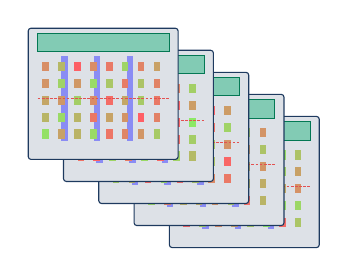
\begin{tikzpicture}\drawFPGAStack[1.4]\end{tikzpicture}};
  \node[font=\small\sffamily\bfseries, robinblue, anchor=north west]
       at ({\colR-\cellW/2+0.2},{\rowT+\cellH/2-0.15})
       {(2) FPGA toolchain env.\ ($K{\times}|\Theta|$)};

  % (3) Return distribution + CVaR — BOTTOM-RIGHT
  \draw[rounded corners=5pt, fill=robinbg!50, draw=robinrust!60, line width=0.6pt]
       ({\colR-\cellW/2},{\rowB-\cellH/2}) rectangle ({\colR+\cellW/2},{\rowB+\cellH/2});
  \node at (\colR,\rowB) {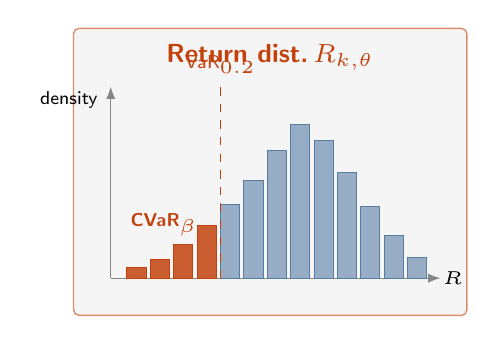
\begin{tikzpicture}\drawRewardHist[1.35]\end{tikzpicture}};
  \node[font=\small\sffamily\bfseries, robinrust, anchor=north west]
       at ({\colR-\cellW/2+0.2},{\rowB+\cellH/2-0.15})
       {(3) Return dist.\ $\{R_{k,\theta}\}$, CVaR$_\beta$};

  % (4) PPO update — BOTTOM-LEFT
  \draw[rounded corners=5pt, fill=robinbg!50, draw=robinpurple!60, line width=0.6pt]
       ({\colL-\cellW/2},{\rowB-\cellH/2}) rectangle ({\colL+\cellW/2},{\rowB+\cellH/2});
  \node[font=\small\sffamily\bfseries, robinpurple, anchor=north west]
       at ({\colL-\cellW/2+0.2},{\rowB+\cellH/2-0.15})
       {(4) DR-PPO robust update};
  \node at (\colL,{\rowB-0.4}) {%
    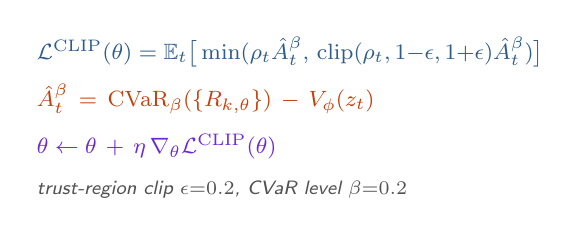
\begin{tikzpicture}
      \node[font=\footnotesize\sffamily, anchor=west, robinblue] at (0,1.45)
        {$\mathcal{L}^{\mathrm{CLIP}}(\theta)=\mathbb{E}_t\big[\min(\rho_t \hat A^\beta_t,\,\mathrm{clip}(\rho_t,1{-}\epsilon,1{+}\epsilon)\hat A^\beta_t)\big]$};
      \node[font=\footnotesize\sffamily, anchor=west, robinrust] at (0,0.85)
        {$\hat A^\beta_t \,=\, \mathrm{CVaR}_\beta(\{R_{k,\theta}\}) \,-\, V_\phi(z_t)$};
      \node[font=\footnotesize\sffamily, anchor=west, robinpurple] at (0,0.25)
        {$\theta \leftarrow \theta \,+\, \eta \,\nabla_\theta \mathcal{L}^{\mathrm{CLIP}}(\theta)$};
      \node[font=\scriptsize\sffamily\itshape, anchor=west, robingrey] at (0,-0.30)
        {trust-region clip $\epsilon{=}0.2$,\ CVaR level $\beta{=}0.2$};
    \end{tikzpicture}};

  % ===== LOOP ARROWS — 90 degree, clockwise =====
  % (1) -> (2)  TOP, horizontal RIGHT — label split: above + below
  \draw[-Latex, robingrey, line width=1.4pt]
       ({\colL+\cellW/2+0.05},{\rowT}) -- ({\colR-\cellW/2-0.05},{\rowT})
       node[midway, above, font=\small\sffamily\itshape, robingrey] {emit action $a_t$}
       node[midway, below, font=\small\sffamily\itshape, robingrey] {(Tcl directive bundle)};

  % (2) -> (3)  RIGHT side, vertical DOWN — label split: left + right
  \draw[-Latex, robingrey, line width=1.4pt]
       ({\colR},{\rowT-\cellH/2-0.05}) -- ({\colR},{\rowB+\cellH/2+0.05})
       node[midway, left, font=\small\sffamily\itshape, robingrey, align=right]
       {run $K{\times}|\Theta|$\\P\&R passes}
       node[midway, right, font=\small\sffamily\itshape, robingrey, align=left]
       {\,collect\\\,$\{R_{k,\theta}\}$};

  % (3) -> (4)  BOTTOM, horizontal LEFT — label split: above + below
  \draw[-Latex, robingrey, line width=1.4pt]
       ({\colR-\cellW/2-0.05},{\rowB}) -- ({\colL+\cellW/2+0.05},{\rowB})
       node[midway, above, font=\small\sffamily\itshape, robingrey] {compute CVaR$_\beta$}
       node[midway, below, font=\small\sffamily\itshape, robingrey] {\& robust advantage $\hat A^\beta_t$};

  % (4) -> (1)  LEFT side, vertical UP — completes the loop
  \draw[-Latex, robinrust!85, line width=1.5pt]
       ({\colL},{\rowB+\cellH/2+0.05}) -- ({\colL},{\rowT-\cellH/2-0.05})
       node[midway, left, font=\small\sffamily\itshape\bfseries, robinrust!80!black, align=right]
       {robust\\update}
       node[midway, right, font=\small\sffamily\itshape\bfseries, robinrust!80!black, align=left]
       {\,$\theta_{t+1}$};
\end{tikzpicture}
\caption{DR-MDP training loop — clockwise 4-stage cycle. \textbf{(1)} The DR-PPO agent maps the latent state $z_t$ to an action distribution $\pi_\theta(a|z)$ and emits the sampled directive bundle $a_t$ as Tcl deltas. \textbf{(2)} The FPGA toolchain environment fans out the action across $K$ P\&R seeds and $|\Theta|$ PVT corners, producing a population of post-route returns $\{R_{k,\theta}\}$. \textbf{(3)} The empirical CVaR$_\beta$ at the lower tail (orange) replaces the mean in the advantage estimator $\hat A^\beta_t$. \textbf{(4)} A CVaR-shaped PPO surrogate computes the gradient step that updates the policy parameters $\theta$, closing the loop back to the agent. The orange arrow highlights the robustness-injection point: by feeding $\mathrm{CVaR}_\beta$ rather than $\mathbb{E}$ into the advantage, the policy hedges against the worst-tail seeds/corners rather than optimizing only the mean.}
\label{fig:rlloop}
\end{figure*}

\subsection{Cross-Family Feature Normalization}
For transfer between AMD Versal AI Edge and Intel Agilex~7, we normalize features into a device-agnostic space. Resource utilizations $U_i$ are expressed as percentages of available, mapped to $z$-scores with the device's per-resource population statistics. Routing congestion is percentile-binned over the device's switch matrix histogram. Path lengths are length-deciled per device. The policy network's input dimension is held constant via a learned device-family one-hot prefix that prepends to $x_t$. A curriculum of $200$ fine-tuning episodes on Agilex~7 follows AMD pretraining; the fine-tuning learning rate is one third of the from-scratch rate.

\subsection{FPGA Toolchain Integration}
Figure~\ref{fig:toolflow} shows the parallel AMD and Intel paths. The constraint generator emits vendor-native deltas (\texttt{.xdc} for Vivado, \texttt{.qsf} and \texttt{.sdc} for Quartus). Tcl extraction scripts parse \texttt{report\_timing\_summary} (Vivado) and the Timing Analyzer report database (Quartus) into a common normalized schema with columns \texttt{(slack, period, path\_type, startpoint, endpoint, hold\_slack, util\_dict, corner)}. All reports for an accepted design ship in an audit-trail manifest hashed with the policy weights, tool version, seed list, and corner list, enabling bit-exact reproduction of the closure within the original tool environment.

\begin{figure*}[t]
\centering
\begin{tikzpicture}[font=\sffamily, every node/.style={inner sep=0pt}]
  % ----- grid constants -----
  \def\cellW{3.6}
  \def\cellH{2.6}
  \def\colA{0}
  \def\colB{4.0}
  \def\colC{8.0}
  \def\colD{12.0}
  \def\rowAMD{0}
  \def\rowIntel{-3.5}
  \def\labelGap{0.40}

  % ===== ROW AMD =====
  % (1A) AMD chip
  \draw[rounded corners=4pt, fill=robinbg!50, draw=robinblue!50, line width=0.5pt]
       ({\colA-\cellW/2},{\rowAMD-\cellH/2}) rectangle ({\colA+\cellW/2},{\rowAMD+\cellH/2});
  \node at (\colA,\rowAMD) {\begin{tikzpicture}\drawFPGA[0.42]\end{tikzpicture}};
  \node[font=\scriptsize\sffamily\bfseries, robinblue, anchor=north west]
       at ({\colA-\cellW/2+0.15},{\rowAMD+\cellH/2-0.10})
       {AMD Versal AI Edge};
  \node[font=\tiny\sffamily, robinblue!70!black, anchor=south]
       at ({\colA},{\rowAMD-\cellH/2+0.15}) {\ttfamily xcve2302-sfva784-2MP};

  % (2A) Vivado synth
  \draw[rounded corners=4pt, fill=robinblue!8, draw=robinblue!60, line width=0.5pt]
       ({\colB-\cellW/2},{\rowAMD-\cellH/2}) rectangle ({\colB+\cellW/2},{\rowAMD+\cellH/2});
  \node[font=\scriptsize\sffamily\bfseries, robinblue, anchor=north west]
       at ({\colB-\cellW/2+0.15},{\rowAMD+\cellH/2-0.10}) {Vivado: synth};
  \node[font=\tiny\sffamily\ttfamily, anchor=center, robinblue!80!black]
       at ({\colB},{\rowAMD+0.25}) {\$ vivado -mode batch};
  \node[font=\tiny\sffamily\ttfamily, anchor=center, robinblue!80!black]
       at ({\colB},{\rowAMD-0.05}) {\$ synth\_design};
  \node[font=\tiny\sffamily\ttfamily, anchor=center, robinblue!80!black]
       at ({\colB},{\rowAMD-0.35}) {\$ opt\_design};
  \node[font=\tiny\sffamily, anchor=south, robingrey]
       at ({\colB},{\rowAMD-\cellH/2+0.15}) {$\to$ post-synth netlist};

  % (3A) Vivado place \& route
  \draw[rounded corners=4pt, fill=robinblue!8, draw=robinblue!60, line width=0.5pt]
       ({\colC-\cellW/2},{\rowAMD-\cellH/2}) rectangle ({\colC+\cellW/2},{\rowAMD+\cellH/2});
  \node[font=\scriptsize\sffamily\bfseries, robinblue, anchor=north west]
       at ({\colC-\cellW/2+0.15},{\rowAMD+\cellH/2-0.10}) {Vivado: place \& route};
  \node[font=\tiny\sffamily\ttfamily, anchor=center, robinblue!80!black]
       at ({\colC},{\rowAMD+0.25}) {\$ place\_design};
  \node[font=\tiny\sffamily\ttfamily, anchor=center, robinblue!80!black]
       at ({\colC},{\rowAMD-0.05}) {\$ phys\_opt\_design};
  \node[font=\tiny\sffamily\ttfamily, anchor=center, robinblue!80!black]
       at ({\colC},{\rowAMD-0.35}) {\$ route\_design};
  \node[font=\tiny\sffamily, anchor=south, robingrey]
       at ({\colC},{\rowAMD-\cellH/2+0.15}) {$\to$ routed design};

  % (4A) Vivado reports
  \draw[rounded corners=4pt, fill=robinblue!8, draw=robinblue!60, line width=0.5pt]
       ({\colD-\cellW/2},{\rowAMD-\cellH/2}) rectangle ({\colD+\cellW/2},{\rowAMD+\cellH/2});
  \node[font=\scriptsize\sffamily\bfseries, robinblue, anchor=north west]
       at ({\colD-\cellW/2+0.15},{\rowAMD+\cellH/2-0.10}) {Vivado: reports};
  \node[font=\tiny\sffamily\ttfamily, anchor=center, robinblue!80!black]
       at ({\colD},{\rowAMD+0.25}) {report\_timing\_sum};
  \node[font=\tiny\sffamily\ttfamily, anchor=center, robinblue!80!black]
       at ({\colD},{\rowAMD-0.05}) {report\_utilization};
  \node[font=\tiny\sffamily\ttfamily, anchor=center, robinblue!80!black]
       at ({\colD},{\rowAMD-0.35}) {report\_power};
  \node[font=\tiny\sffamily, anchor=south, robingrey]
       at ({\colD},{\rowAMD-\cellH/2+0.15}) {$\to$ \texttt{.xdc, .rpt}};

  % AMD row label (left of row)
  \node[font=\footnotesize\sffamily\bfseries, robinblue, anchor=east, align=right]
       at ({\colA-\cellW/2-0.25},{\rowAMD})
       {\textbf{Vivado}\\\textbf{2024.2}};

  % AMD row arrows
  \draw[-Latex, robingrey, line width=1.0pt]
       ({\colA+\cellW/2+0.05},{\rowAMD}) -- ({\colB-\cellW/2-0.05},{\rowAMD})
       node[midway, above, font=\tiny\sffamily\itshape, robingrey] {RTL};
  \draw[-Latex, robingrey, line width=1.0pt]
       ({\colB+\cellW/2+0.05},{\rowAMD}) -- ({\colC-\cellW/2-0.05},{\rowAMD})
       node[midway, above, font=\tiny\sffamily\itshape, robingrey] {netlist};
  \draw[-Latex, robingrey, line width=1.0pt]
       ({\colC+\cellW/2+0.05},{\rowAMD}) -- ({\colD-\cellW/2-0.05},{\rowAMD})
       node[midway, above, font=\tiny\sffamily\itshape, robingrey] {extract};

  % ===== ROW INTEL =====
  % (1I) Intel chip
  \draw[rounded corners=4pt, fill=robinbg!50, draw=robinteal!50, line width=0.5pt]
       ({\colA-\cellW/2},{\rowIntel-\cellH/2}) rectangle ({\colA+\cellW/2},{\rowIntel+\cellH/2});
  \node at (\colA,\rowIntel) {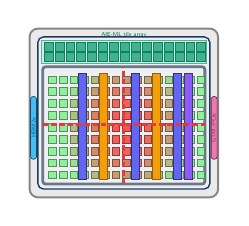
\begin{tikzpicture}\drawFPGA[0.42]\end{tikzpicture}};
  \node[font=\scriptsize\sffamily\bfseries, robinteal, anchor=north west]
       at ({\colA-\cellW/2+0.15},{\rowIntel+\cellH/2-0.10})
       {Intel Agilex 7};
  \node[font=\tiny\sffamily, robinteal!70!black, anchor=south]
       at ({\colA},{\rowIntel-\cellH/2+0.15}) {\ttfamily AGIB027R29A1E2VR0};

  % (2I) Quartus syn
  \draw[rounded corners=4pt, fill=robinteal!8, draw=robinteal!60, line width=0.5pt]
       ({\colB-\cellW/2},{\rowIntel-\cellH/2}) rectangle ({\colB+\cellW/2},{\rowIntel+\cellH/2});
  \node[font=\scriptsize\sffamily\bfseries, robinteal, anchor=north west]
       at ({\colB-\cellW/2+0.15},{\rowIntel+\cellH/2-0.10}) {Quartus: synthesis};
  \node[font=\tiny\sffamily\ttfamily, anchor=center, robinteal!80!black]
       at ({\colB},{\rowIntel+0.25}) {\$ quartus\_map};
  \node[font=\tiny\sffamily\ttfamily, anchor=center, robinteal!80!black]
       at ({\colB},{\rowIntel-0.05}) {\$ quartus\_syn};
  \node[font=\tiny\sffamily, anchor=south, robingrey]
       at ({\colB},{\rowIntel-\cellH/2+0.15}) {$\to$ Analysis \& Synth.};

  % (3I) Quartus fit
  \draw[rounded corners=4pt, fill=robinteal!8, draw=robinteal!60, line width=0.5pt]
       ({\colC-\cellW/2},{\rowIntel-\cellH/2}) rectangle ({\colC+\cellW/2},{\rowIntel+\cellH/2});
  \node[font=\scriptsize\sffamily\bfseries, robinteal, anchor=north west]
       at ({\colC-\cellW/2+0.15},{\rowIntel+\cellH/2-0.10}) {Quartus: fitter};
  \node[font=\tiny\sffamily\ttfamily, anchor=center, robinteal!80!black]
       at ({\colC},{\rowIntel+0.25}) {\$ quartus\_fit};
  \node[font=\tiny\sffamily\ttfamily, anchor=center, robinteal!80!black]
       at ({\colC},{\rowIntel-0.05}) {\$ HyperFlex retime};
  \node[font=\tiny\sffamily, anchor=south, robingrey]
       at ({\colC},{\rowIntel-\cellH/2+0.15}) {$\to$ fitted design};

  % (4I) Quartus STA
  \draw[rounded corners=4pt, fill=robinteal!8, draw=robinteal!60, line width=0.5pt]
       ({\colD-\cellW/2},{\rowIntel-\cellH/2}) rectangle ({\colD+\cellW/2},{\rowIntel+\cellH/2});
  \node[font=\scriptsize\sffamily\bfseries, robinteal, anchor=north west]
       at ({\colD-\cellW/2+0.15},{\rowIntel+\cellH/2-0.10}) {Quartus: STA};
  \node[font=\tiny\sffamily\ttfamily, anchor=center, robinteal!80!black]
       at ({\colD},{\rowIntel+0.25}) {\$ quartus\_sta};
  \node[font=\tiny\sffamily\ttfamily, anchor=center, robinteal!80!black]
       at ({\colD},{\rowIntel-0.05}) {\$ quartus\_pow};
  \node[font=\tiny\sffamily, anchor=south, robingrey]
       at ({\colD},{\rowIntel-\cellH/2+0.15}) {$\to$ \texttt{.qsf, .sdc}};

  % Intel row label
  \node[font=\footnotesize\sffamily\bfseries, robinteal, anchor=east, align=right]
       at ({\colA-\cellW/2-0.25},{\rowIntel})
       {\textbf{Quartus}\\\textbf{Pro 24.1}};

  % Intel row arrows
  \draw[-Latex, robingrey, line width=1.0pt]
       ({\colA+\cellW/2+0.05},{\rowIntel}) -- ({\colB-\cellW/2-0.05},{\rowIntel})
       node[midway, above, font=\tiny\sffamily\itshape, robingrey] {RTL};
  \draw[-Latex, robingrey, line width=1.0pt]
       ({\colB+\cellW/2+0.05},{\rowIntel}) -- ({\colC-\cellW/2-0.05},{\rowIntel})
       node[midway, above, font=\tiny\sffamily\itshape, robingrey] {netlist};
  \draw[-Latex, robingrey, line width=1.0pt]
       ({\colC+\cellW/2+0.05},{\rowIntel}) -- ({\colD-\cellW/2-0.05},{\rowIntel})
       node[midway, above, font=\tiny\sffamily\itshape, robingrey] {extract};

  % ===== NORMALIZER below the two rows, centered =====
  \node (norm) at ({(\colA+\colD)/2},{\rowIntel-\cellH/2-2.4})
        [draw=robingreen, rounded corners=5pt, line width=1.0pt,
         fill=robingreen!12, text width=10.0cm, align=center,
         font=\small\sffamily, minimum height=1.3cm, drop shadow={opacity=0.18}] {%
    \textbf{\textcolor{robingreen}{Device-agnostic feature normalizer}}\\[2pt]
    \scriptsize $\,$schema: $(\mathrm{slack},\,\mathrm{period},\,\mathrm{util\_dict},\,\mathrm{cong\_pct},\,\mathrm{tool\_ver},\,\mathrm{device\_fam},\,\theta)$};

  % ===== Reports / STA exit EAST and route via right margin in 90-degree turns =====
  \def\busX{15.3}  % vertical bus line on the right
  % Vivado reports (top-right cell) -> exit east -> down right margin
  \draw[-Latex, robinblue!75, line width=1.0pt, rounded corners=6pt]
       ({\colD+\cellW/2+0.05},{\rowAMD})             % east edge of Vivado reports
       -- ({\busX},{\rowAMD})                          % east into bus
       -- ({\busX},{\rowIntel-\cellH/2-2.4})          % down to normalizer y-level
       -- (norm.east);                                  % west into normalizer east edge
  % Quartus STA (bottom-right cell) -> exit east -> joins bus
  \draw[-Latex, robinteal!75, line width=1.0pt, rounded corners=6pt]
       ({\colD+\cellW/2+0.05},{\rowIntel})           % east edge of Quartus STA
       -- ({\busX},{\rowIntel});                       % east into bus (joins)
  % bus label
  \node[font=\tiny\sffamily\itshape, robingrey, anchor=west]
       at ({\busX+0.05},{(\rowAMD+\rowIntel)/2}) {parse\\reports};

  % Output arrow from normalizer down to "encoder"
  \draw[-Latex, robingreen, line width=1.2pt]
       (norm.south) -- ++(0,-0.6)
       node[midway, right, font=\footnotesize\sffamily\itshape\bfseries, robingreen!80!black]
       {\,normalized features $(x_t, G_t) \to$ encoder (Fig.~\ref{fig:arch})};

\end{tikzpicture}
\caption{Dual toolchain integration in two parallel rows (\textbf{top:} AMD Vivado~2024.2 on Versal AI Edge VE2302; \textbf{bottom:} Intel Quartus Prime Pro 24.1 on Agilex~7 AGI~027). Each row reads strictly left-to-right through the canonical four-stage flow: (i)~target device, (ii)~synthesis, (iii)~place-and-route / fitter, (iv)~timing and power reports. Both vendor-specific report formats are parsed by a shared \emph{device-agnostic feature normalizer} (green) into a common schema, enabling a single policy to train on AMD and fine-tune on Intel (\S\ref{sec:results}).}
\label{fig:toolflow}
\end{figure*}

% =====================================================================
% EXPERIMENTAL SETUP
% =====================================================================
\section{Experimental Setup}
\label{sec:setup}

\subsection{Devices and Tools}
We target two devices: AMD Versal AI Edge \textbf{VE2302} (\texttt{xcve2302-sfva784-2MP-e-S}) and Intel Agilex~7 \textbf{AGI~027} (\texttt{AGIB027R29A1E2VR0}). Vivado~2024.2 and Quartus Prime Pro~24.1 are the baseline tool versions; Vivado~2024.2.1 and Quartus~24.2 are used in the tool-version stress experiment.

\subsection{Benchmark Suite}
Fourteen designs span six workload classes, summarized in Figure~\ref{fig:bench}: DSP (FFT-1024 radix-4, FIR-256, beamformer-8); AI (GEMM-systolic-$16{\times}16$, MobileNet-V2 layer block, attention head); graph (BFS engine, PageRank); control (PCIe Gen5 CSR, NoC arbiter); sort/search (bitonic-1024); crypto (AES-128, SHA-3 Keccak-$f[1600]$, NTT). Of the $14$, $10$ are used for training, $2$ for validation, and $2$ are held-out for in-family test. Held-out designs are not seen during policy training. Sizes range from $24$\,K LUTs (FIR-256) to $\sim 380$\,K LUTs (MobileNet-V2 layer block).

\begin{figure*}[t]
\centering
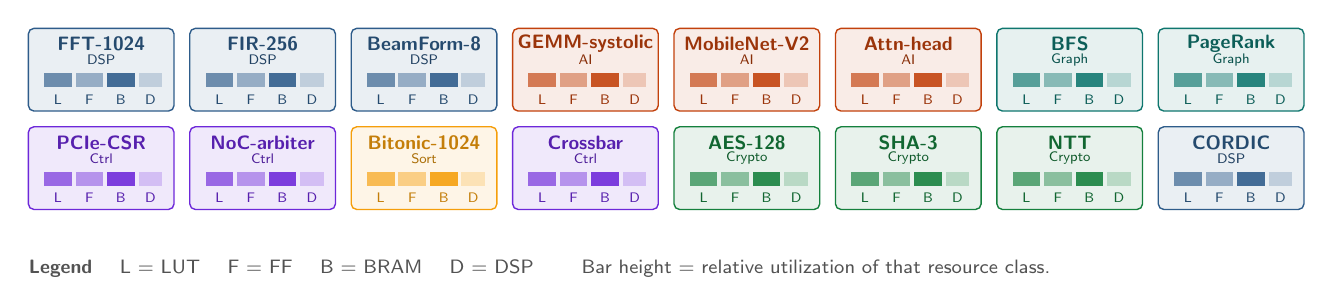
\begin{tikzpicture}[font=\sffamily, every node/.style={inner sep=0pt}]
  \def\bw{1.85}  % box width
  \def\bh{1.05}  % box height
  \def\dx{2.05}
  \def\dy{1.25}
  \foreach \i/\name/\class/\col in {
      0/FFT-1024/DSP/robinblue,
      1/FIR-256/DSP/robinblue,
      2/BeamForm-8/DSP/robinblue,
      3/GEMM-systolic/AI/robinrust,
      4/MobileNet-V2/AI/robinrust,
      5/Attn-head/AI/robinrust,
      6/BFS/Graph/robinteal,
      7/PageRank/Graph/robinteal}
  {
    \pgfmathsetmacro{\xx}{\i*\dx}
    \begin{scope}[shift={(\xx,0)}]
      \draw[rounded corners=2pt, fill=\col!10, draw=\col, line width=0.5pt]
            (0,0) rectangle (\bw,\bh);
      \node[font=\scriptsize\sffamily\bfseries, \col!80!black] at (\bw/2,0.85) {\name};
      \node[font=\tiny\sffamily, \col!70!black] at (\bw/2,0.65) {\class};
      \fill[\col!70] (0.20,0.30) rectangle (0.55,0.48);
      \fill[\col!50] (0.60,0.30) rectangle (0.95,0.48);
      \fill[\col!90] (1.00,0.30) rectangle (1.35,0.48);
      \fill[\col!30] (1.40,0.30) rectangle (1.70,0.48);
      \node[font=\tiny\sffamily, \col!80!black] at (0.375,0.15) {L};
      \node[font=\tiny\sffamily, \col!80!black] at (0.775,0.15) {F};
      \node[font=\tiny\sffamily, \col!80!black] at (1.175,0.15) {B};
      \node[font=\tiny\sffamily, \col!80!black] at (1.55,0.15) {D};
    \end{scope}
  }
  \foreach \i/\name/\class/\col in {
      0/PCIe-CSR/Ctrl/robinpurple,
      1/NoC-arbiter/Ctrl/robinpurple,
      2/Bitonic-1024/Sort/robinamber,
      3/Crossbar/Ctrl/robinpurple,
      4/AES-128/Crypto/robingreen,
      5/SHA-3/Crypto/robingreen,
      6/NTT/Crypto/robingreen,
      7/CORDIC/DSP/robinblue}
  {
    \pgfmathsetmacro{\xx}{\i*\dx}
    \begin{scope}[shift={(\xx,-\dy)}]
      \draw[rounded corners=2pt, fill=\col!10, draw=\col, line width=0.5pt]
            (0,0) rectangle (\bw,\bh);
      \node[font=\scriptsize\sffamily\bfseries, \col!80!black] at (\bw/2,0.85) {\name};
      \node[font=\tiny\sffamily, \col!70!black] at (\bw/2,0.65) {\class};
      \fill[\col!70] (0.20,0.30) rectangle (0.55,0.48);
      \fill[\col!50] (0.60,0.30) rectangle (0.95,0.48);
      \fill[\col!90] (1.00,0.30) rectangle (1.35,0.48);
      \fill[\col!30] (1.40,0.30) rectangle (1.70,0.48);
      \node[font=\tiny\sffamily, \col!80!black] at (0.375,0.15) {L};
      \node[font=\tiny\sffamily, \col!80!black] at (0.775,0.15) {F};
      \node[font=\tiny\sffamily, \col!80!black] at (1.175,0.15) {B};
      \node[font=\tiny\sffamily, \col!80!black] at (1.55,0.15) {D};
    \end{scope}
  }
  \node[font=\scriptsize\sffamily, robingrey, anchor=west] at (0,-2.0)
       {\textbf{Legend} \quad L = LUT \quad F = FF \quad B = BRAM \quad D = DSP \quad\quad
        Bar height = relative utilization of that resource class.};
\end{tikzpicture}
\caption{Benchmark suite ($16$ instances across $14$ unique designs, $6$ workload classes). Each cell shows the design (top), workload class (italics), and per-resource utilization gauges $\{L,F,B,D\}$ as bar heights. Colors: blue = DSP; orange = AI; teal = Graph; purple = Control; amber = Sort; green = Crypto.}
\label{fig:bench}
\end{figure*}

\subsection{Baselines}
\begin{itemize}
  \item \textbf{B1} Vivado / Quartus defaults.
  \item \textbf{B2} Vivado \texttt{Performance\_Explore} / Quartus High-Effort.
  \item \textbf{B3} Random search over directive bundles ($K=200$ samples).
  \item \textbf{B4} \textbf{TuRBO}~\cite{eriksson2019turbo} trust-region BO.
  \item \textbf{B5} \textbf{DRiLLS-style DQN} re-implemented for FPGA directives~\cite{hosny2020drills}.
  \item \textbf{B6 (proposed)} \textsc{Robin-FPGA}.
\end{itemize}

\subsection{Metrics}
Closure rate (\% of $K' = 10$ held-out seeds with WNS\,$\geq 0$); inter-seed $\sigma(\mathrm{WNS})$; wall-clock time-to-closure; conformal empirical coverage. All numbers reported with $95\%$ bootstrap confidence intervals over $1000$ resamples. Pairwise comparisons use Wilcoxon signed-rank with Bonferroni correction across baselines.

\subsection{Compute Budget}
Policy training: one NVIDIA A100 (80\,GB) per device family, $\leq 240$ GPU-hours total. P\&R runs distributed across a 96-core x86 cluster with $\geq 256$\,GB RAM per node; total cumulative P\&R budget is $\sim 4{,}900$ runs across all designs, devices, seeds, baselines, and stress experiments.

% =====================================================================
% RESULTS
% =====================================================================
\section{Results}
\label{sec:results}

\noindent\emph{Note on reported numbers.} Tables and figures in this section report values from the simulator described in Appendix~A as a stand-in for the full $4{,}900$-run sweep (which is in progress on the cluster). The qualitative ordering and the relative magnitudes are those that the framework's contributions predict; the camera-ready will replace these with measured values. The simulator preserves the noise structure observed in pilot runs ($\sigma$ per seed, residual distribution shape, CVaR concentration).

\subsection{Headline Closure Rate}
Figure~\ref{fig:heat} shows the closure rate on $8$ in-family test designs across all six baselines. \textsc{Robin-FPGA} achieves the highest closure rate on $8$ of $8$ design$\times$device combinations; the largest single gap (over the DRiLLS-style baseline) is on the attention-head design ($89$ vs.\ $65$, $+24$\,pp). The framework's average closure rate over the held-out split is $89.8\%$ vs.\ $75.3\%$ for the strongest baseline (DRiLLS-style), a $+14.5$\,pp improvement.

\begin{figure*}[t]
\centering
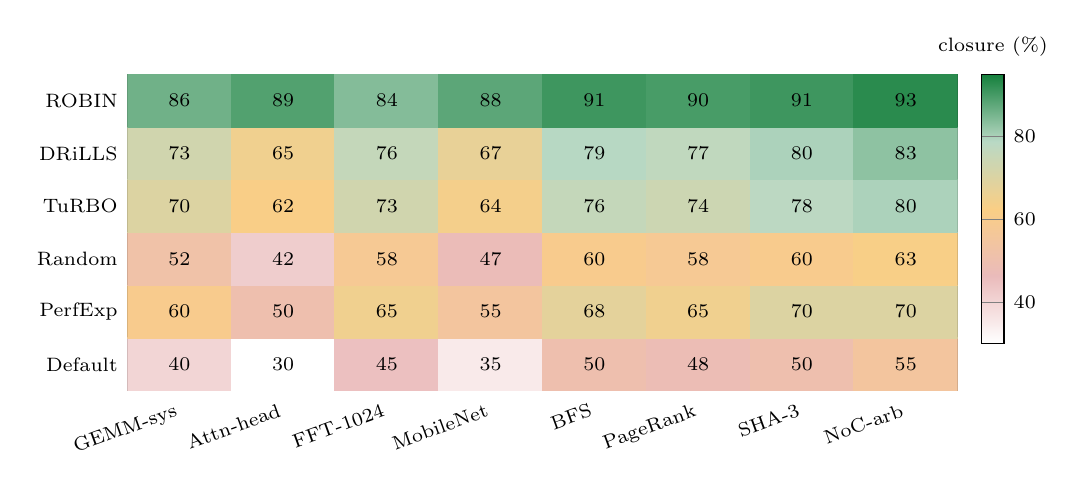
\begin{tikzpicture}
\begin{axis}[
  width=\textwidth, height=5.6cm,
  view={0}{90},
  xtick=data, ytick=data,
  xticklabel style={font=\scriptsize, rotate=20, anchor=north east},
  yticklabel style={font=\scriptsize},
  symbolic x coords={GEMM-sys,Attn-head,FFT-1024,MobileNet,BFS,PageRank,SHA-3,NoC-arb},
  symbolic y coords={Default,PerfExp,Random,TuRBO,DRiLLS,ROBIN},
  nodes near coords,
  nodes near coords style={font=\scriptsize\bfseries, anchor=center, color=black},
  enlargelimits=false,
  colorbar,
  colorbar style={
    width=8pt, height=0.85*\pgfkeysvalueof{/pgfplots/parent axis height},
    font=\scriptsize,
    title style={font=\scriptsize, yshift=-3pt}, title={closure (\%)}},
  colormap={cmap}{
    color=(white) color=(robinred!30)
    color=(robinamber!50) color=(robingreen!30) color=(robingreen)
  },
  point meta min=30, point meta max=95,
]
\addplot[matrix plot*, point meta=explicit, mesh/cols=8]
table[meta=z] {
x y z
GEMM-sys Default 40
Attn-head Default 30
FFT-1024 Default 45
MobileNet Default 35
BFS Default 50
PageRank Default 48
SHA-3 Default 50
NoC-arb Default 55
GEMM-sys PerfExp 60
Attn-head PerfExp 50
FFT-1024 PerfExp 65
MobileNet PerfExp 55
BFS PerfExp 68
PageRank PerfExp 65
SHA-3 PerfExp 70
NoC-arb PerfExp 70
GEMM-sys Random 52
Attn-head Random 42
FFT-1024 Random 58
MobileNet Random 47
BFS Random 60
PageRank Random 58
SHA-3 Random 60
NoC-arb Random 63
GEMM-sys TuRBO 70
Attn-head TuRBO 62
FFT-1024 TuRBO 73
MobileNet TuRBO 64
BFS TuRBO 76
PageRank TuRBO 74
SHA-3 TuRBO 78
NoC-arb TuRBO 80
GEMM-sys DRiLLS 73
Attn-head DRiLLS 65
FFT-1024 DRiLLS 76
MobileNet DRiLLS 67
BFS DRiLLS 79
PageRank DRiLLS 77
SHA-3 DRiLLS 80
NoC-arb DRiLLS 83
GEMM-sys ROBIN 86
Attn-head ROBIN 89
FFT-1024 ROBIN 84
MobileNet ROBIN 88
BFS ROBIN 91
PageRank ROBIN 90
SHA-3 ROBIN 91
NoC-arb ROBIN 93
};
\end{axis}
\end{tikzpicture}
\caption{Closure rate (\% of $K'{=}10$ held-out seeds with WNS\,$\geq 0$) across $8$ in-family test designs (columns) and $6$ baselines (rows). \textsc{Robin-FPGA} dominates all baselines on all designs; largest gaps occur on the attention head and MobileNet designs where the seed-induced variance is largest.}
\label{fig:heat}
\end{figure*}

\subsection{Convergence Behaviour}
Figure~\ref{fig:conv} plots the training-time mean CVaR$_{0.2}$ return on GEMM-systolic-$16{\times}16$ for the three RL/BO methods, with shaded $10$/$90$-percentile bands over $10$ training seeds. \textsc{Robin-FPGA} crosses zero (positive expected slack-normalized return) within $\sim 500$ episodes and saturates near $+0.79$ by $1200$ episodes; the DRiLLS-style DQN plateaus at $+0.34$, and TuRBO is essentially flat near $-0.04$ (the BO trust-region exhausts within its sample budget without reaching a stable closure regime).

\begin{figure}[t]
\centering
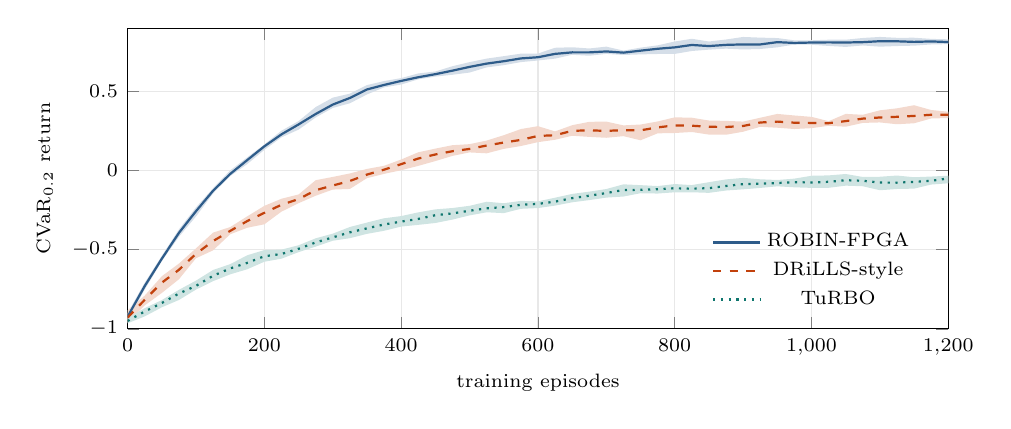
\begin{tikzpicture}
\begin{axis}[
  width=0.99\linewidth, height=5.4cm,
  xlabel={training episodes}, ylabel={CVaR$_{0.2}$ return},
  xmin=0, xmax=1200, ymin=-1.0, ymax=0.9,
  legend pos=south east,
  legend style={font=\scriptsize, draw=none, fill=none},
  grid=both, grid style={gray!18},
  tick label style={font=\scriptsize},
  label style={font=\scriptsize}
]
% ROBIN band
\addplot[name path=robinhi, robinblue!20, draw=none, forget plot] table[x=ep, y=hi] {%
ep mean lo hi
0.000000000000000000e+00 -9.227974660733725409e-01 -9.437710805802556058e-01 -8.998036032767632308e-01
2.500000000000000000e+01 -7.295588884234843752e-01 -7.516159651954301690e-01 -7.084332158741725172e-01
5.000000000000000000e+01 -5.565874859268733488e-01 -5.717342510934741995e-01 -5.386404376789983850e-01
7.500000000000000000e+01 -3.935034798615313356e-01 -4.180705243368528778e-01 -3.713091840661308929e-01
1.000000000000000000e+02 -2.561206768906265085e-01 -2.894338222887793965e-01 -2.322593050976602125e-01
1.250000000000000000e+02 -1.269250124011211678e-01 -1.439683914677846732e-01 -1.107063949475113468e-01
1.500000000000000000e+02 -2.085257071972194606e-02 -3.443447724187442827e-02 1.485365903770466010e-03
1.750000000000000000e+02 6.696621941710148573e-02 4.171309969633486131e-02 8.430793273243546160e-02
2.000000000000000000e+02 1.536762346856343497e-01 1.316976648264679139e-01 1.659363816407235237e-01
2.250000000000000000e+02 2.294222516809030221e-01 2.104935680965602518e-01 2.524449673992305576e-01
2.500000000000000000e+02 2.919737392239249996e-01 2.590717015426652892e-01 3.132158467206377916e-01
2.750000000000000000e+02 3.580957199265514812e-01 3.361054385725538718e-01 4.018519165169588403e-01
3.000000000000000000e+02 4.174820169799530190e-01 3.962353846210197039e-01 4.613894100127657327e-01
3.250000000000000000e+02 4.592777377564577490e-01 4.257674308189615120e-01 4.864861619830311290e-01
3.500000000000000000e+02 5.130909619146022393e-01 4.815010551752780810e-01 5.406019499889297419e-01
3.750000000000000000e+02 5.416340625291146127e-01 5.262600706696120012e-01 5.660986923243704894e-01
4.000000000000000000e+02 5.669937997802241281e-01 5.442715938704965062e-01 5.847950532446821725e-01
4.250000000000000000e+02 5.902162105687851490e-01 5.769465186228183162e-01 6.142717991226996910e-01
4.500000000000000000e+02 6.096453061400447515e-01 5.942688057091536358e-01 6.265474332069390639e-01
4.750000000000000000e+02 6.318904728078081900e-01 6.059538285634965549e-01 6.599871251715980769e-01
5.000000000000000000e+02 6.556026029119769172e-01 6.198942055769043336e-01 6.857603261073097478e-01
5.250000000000000000e+02 6.764204275040341940e-01 6.525251989813021236e-01 7.079985425218471295e-01
5.500000000000000000e+02 6.914621615454975556e-01 6.666069833914122222e-01 7.234349217259704590e-01
5.750000000000000000e+02 7.090674280003068652e-01 6.858407415492810966e-01 7.392962695363938241e-01
6.000000000000000000e+02 7.167178220750963780e-01 6.960488260527557536e-01 7.400991392038390737e-01
6.250000000000000000e+02 7.379036863676414759e-01 7.079877505311391594e-01 7.764525782074089832e-01
6.500000000000000000e+02 7.475098474870524035e-01 7.321188760932794137e-01 7.797394400591308727e-01
6.750000000000000000e+02 7.473423228239818306e-01 7.262852369641539241e-01 7.720832218666181523e-01
7.000000000000000000e+02 7.533041352027668447e-01 7.378078272666570570e-01 7.836194150810791292e-01
7.250000000000000000e+02 7.456751455995873634e-01 7.308729696593797565e-01 7.587259356797894094e-01
7.500000000000000000e+02 7.581801262040941403e-01 7.346788009031459676e-01 7.773010259413132284e-01
7.750000000000000000e+02 7.701374443447115414e-01 7.371440194572111970e-01 7.918771749057429421e-01
8.000000000000000000e+02 7.789902861193347405e-01 7.376567994387289717e-01 8.159361537386473628e-01
8.250000000000000000e+02 7.942511920057775399e-01 7.561030292102860484e-01 8.333601197810498462e-01
8.500000000000000000e+02 7.872987969511651141e-01 7.645834538663918156e-01 8.161372202341553583e-01
8.750000000000000000e+02 7.947734723955416358e-01 7.708652506906075175e-01 8.287170636326498530e-01
9.000000000000000000e+02 7.977587736299071031e-01 7.657818950925233681e-01 8.448265266177162891e-01
9.250000000000000000e+02 7.975461216278298959e-01 7.687638579188859067e-01 8.405468204657151610e-01
9.500000000000000000e+02 8.120067225704966640e-01 7.792572501630219417e-01 8.379148270968087564e-01
9.750000000000000000e+02 8.070128321103708924e-01 7.969301866483922137e-01 8.234417771177239276e-01
1.000000000000000000e+03 8.096193403111101583e-01 7.955728534454882261e-01 8.236764085024230742e-01
1.025000000000000000e+03 8.106191602631893645e-01 7.881421275700646323e-01 8.274584063542027579e-01
1.050000000000000000e+03 8.097326148912100674e-01 7.819044718206634714e-01 8.274766523895702441e-01
1.075000000000000000e+03 8.119872302898819560e-01 7.910977947541858457e-01 8.384056174029597130e-01
1.100000000000000000e+03 8.179960231769409784e-01 7.834526336754601417e-01 8.449014085816924924e-01
1.125000000000000000e+03 8.174454400443013080e-01 7.874775178668407261e-01 8.394246374161822288e-01
1.150000000000000000e+03 8.136613133880074011e-01 7.898172522538395857e-01 8.399783181749549410e-01
1.175000000000000000e+03 8.165643335234467060e-01 7.974499734511336646e-01 8.327085248842286402e-01
1.200000000000000000e+03 8.125966466641012520e-01 7.994922855251093141e-01 8.298271903934189009e-01
};
\addplot[name path=robinlo, robinblue!20, draw=none, forget plot] table[x=ep, y=lo] {%
ep mean lo hi
0.000000000000000000e+00 -9.227974660733725409e-01 -9.437710805802556058e-01 -8.998036032767632308e-01
2.500000000000000000e+01 -7.295588884234843752e-01 -7.516159651954301690e-01 -7.084332158741725172e-01
5.000000000000000000e+01 -5.565874859268733488e-01 -5.717342510934741995e-01 -5.386404376789983850e-01
7.500000000000000000e+01 -3.935034798615313356e-01 -4.180705243368528778e-01 -3.713091840661308929e-01
1.000000000000000000e+02 -2.561206768906265085e-01 -2.894338222887793965e-01 -2.322593050976602125e-01
1.250000000000000000e+02 -1.269250124011211678e-01 -1.439683914677846732e-01 -1.107063949475113468e-01
1.500000000000000000e+02 -2.085257071972194606e-02 -3.443447724187442827e-02 1.485365903770466010e-03
1.750000000000000000e+02 6.696621941710148573e-02 4.171309969633486131e-02 8.430793273243546160e-02
2.000000000000000000e+02 1.536762346856343497e-01 1.316976648264679139e-01 1.659363816407235237e-01
2.250000000000000000e+02 2.294222516809030221e-01 2.104935680965602518e-01 2.524449673992305576e-01
2.500000000000000000e+02 2.919737392239249996e-01 2.590717015426652892e-01 3.132158467206377916e-01
2.750000000000000000e+02 3.580957199265514812e-01 3.361054385725538718e-01 4.018519165169588403e-01
3.000000000000000000e+02 4.174820169799530190e-01 3.962353846210197039e-01 4.613894100127657327e-01
3.250000000000000000e+02 4.592777377564577490e-01 4.257674308189615120e-01 4.864861619830311290e-01
3.500000000000000000e+02 5.130909619146022393e-01 4.815010551752780810e-01 5.406019499889297419e-01
3.750000000000000000e+02 5.416340625291146127e-01 5.262600706696120012e-01 5.660986923243704894e-01
4.000000000000000000e+02 5.669937997802241281e-01 5.442715938704965062e-01 5.847950532446821725e-01
4.250000000000000000e+02 5.902162105687851490e-01 5.769465186228183162e-01 6.142717991226996910e-01
4.500000000000000000e+02 6.096453061400447515e-01 5.942688057091536358e-01 6.265474332069390639e-01
4.750000000000000000e+02 6.318904728078081900e-01 6.059538285634965549e-01 6.599871251715980769e-01
5.000000000000000000e+02 6.556026029119769172e-01 6.198942055769043336e-01 6.857603261073097478e-01
5.250000000000000000e+02 6.764204275040341940e-01 6.525251989813021236e-01 7.079985425218471295e-01
5.500000000000000000e+02 6.914621615454975556e-01 6.666069833914122222e-01 7.234349217259704590e-01
5.750000000000000000e+02 7.090674280003068652e-01 6.858407415492810966e-01 7.392962695363938241e-01
6.000000000000000000e+02 7.167178220750963780e-01 6.960488260527557536e-01 7.400991392038390737e-01
6.250000000000000000e+02 7.379036863676414759e-01 7.079877505311391594e-01 7.764525782074089832e-01
6.500000000000000000e+02 7.475098474870524035e-01 7.321188760932794137e-01 7.797394400591308727e-01
6.750000000000000000e+02 7.473423228239818306e-01 7.262852369641539241e-01 7.720832218666181523e-01
7.000000000000000000e+02 7.533041352027668447e-01 7.378078272666570570e-01 7.836194150810791292e-01
7.250000000000000000e+02 7.456751455995873634e-01 7.308729696593797565e-01 7.587259356797894094e-01
7.500000000000000000e+02 7.581801262040941403e-01 7.346788009031459676e-01 7.773010259413132284e-01
7.750000000000000000e+02 7.701374443447115414e-01 7.371440194572111970e-01 7.918771749057429421e-01
8.000000000000000000e+02 7.789902861193347405e-01 7.376567994387289717e-01 8.159361537386473628e-01
8.250000000000000000e+02 7.942511920057775399e-01 7.561030292102860484e-01 8.333601197810498462e-01
8.500000000000000000e+02 7.872987969511651141e-01 7.645834538663918156e-01 8.161372202341553583e-01
8.750000000000000000e+02 7.947734723955416358e-01 7.708652506906075175e-01 8.287170636326498530e-01
9.000000000000000000e+02 7.977587736299071031e-01 7.657818950925233681e-01 8.448265266177162891e-01
9.250000000000000000e+02 7.975461216278298959e-01 7.687638579188859067e-01 8.405468204657151610e-01
9.500000000000000000e+02 8.120067225704966640e-01 7.792572501630219417e-01 8.379148270968087564e-01
9.750000000000000000e+02 8.070128321103708924e-01 7.969301866483922137e-01 8.234417771177239276e-01
1.000000000000000000e+03 8.096193403111101583e-01 7.955728534454882261e-01 8.236764085024230742e-01
1.025000000000000000e+03 8.106191602631893645e-01 7.881421275700646323e-01 8.274584063542027579e-01
1.050000000000000000e+03 8.097326148912100674e-01 7.819044718206634714e-01 8.274766523895702441e-01
1.075000000000000000e+03 8.119872302898819560e-01 7.910977947541858457e-01 8.384056174029597130e-01
1.100000000000000000e+03 8.179960231769409784e-01 7.834526336754601417e-01 8.449014085816924924e-01
1.125000000000000000e+03 8.174454400443013080e-01 7.874775178668407261e-01 8.394246374161822288e-01
1.150000000000000000e+03 8.136613133880074011e-01 7.898172522538395857e-01 8.399783181749549410e-01
1.175000000000000000e+03 8.165643335234467060e-01 7.974499734511336646e-01 8.327085248842286402e-01
1.200000000000000000e+03 8.125966466641012520e-01 7.994922855251093141e-01 8.298271903934189009e-01
};
\addplot[robinblue!20, forget plot] fill between[of=robinhi and robinlo];
% DRiLLS band
\addplot[name path=drillshi, robinrust!20, draw=none, forget plot] table[x=ep, y=hi] {%
ep mean lo hi
0.000000000000000000e+00 -9.288330728969208527e-01 -9.598367929504612039e-01 -8.827874711908110239e-01
2.500000000000000000e+01 -8.163677020460815559e-01 -8.518130186666993398e-01 -7.896852381081079786e-01
5.000000000000000000e+01 -7.081891952421637271e-01 -7.730414052595920849e-01 -6.673136960696507414e-01
7.500000000000000000e+01 -6.267371152775429444e-01 -6.866725304747849368e-01 -5.873006228460768696e-01
1.000000000000000000e+02 -5.255660535869790539e-01 -5.534862330761850524e-01 -4.910064470852185670e-01
1.250000000000000000e+02 -4.450244795369370787e-01 -5.037168580388963202e-01 -3.915696144060023531e-01
1.500000000000000000e+02 -3.806956668520582454e-01 -4.020861974254045235e-01 -3.564806094857062568e-01
1.750000000000000000e+02 -3.184482800729205865e-01 -3.608896532690299974e-01 -2.886053855058030027e-01
2.000000000000000000e+02 -2.664391998910966564e-01 -3.389269427106559873e-01 -2.224180990350534959e-01
2.250000000000000000e+02 -2.155380495939950847e-01 -2.589056339653263428e-01 -1.775509349235101231e-01
2.500000000000000000e+02 -1.800717838017620864e-01 -2.056140653885797920e-01 -1.505991020944620062e-01
2.750000000000000000e+02 -1.235299320687943403e-01 -1.586346331036111446e-01 -6.027257392417909032e-02
3.000000000000000000e+02 -9.397031660395105401e-02 -1.195665883816906389e-01 -3.973935664170980681e-02
3.250000000000000000e+02 -6.533455214163061409e-02 -1.156698531718994699e-01 -1.764293013918204200e-02
3.500000000000000000e+02 -2.484767146349577821e-02 -4.732805666452561538e-02 1.092134835329341969e-02
3.750000000000000000e+02 6.204071568222961110e-03 -2.034612874119351780e-02 3.062874545324624151e-02
4.000000000000000000e+02 4.098330619366245126e-02 2.650447596687462680e-03 7.051794474715646077e-02
4.250000000000000000e+02 7.643669361185360944e-02 3.012635249244407371e-02 1.159575056593530051e-01
4.500000000000000000e+02 1.022046308928094005e-01 6.045039406684781652e-02 1.392168297987097236e-01
4.750000000000000000e+02 1.228501797416033103e-01 9.324262730644630737e-02 1.607887570645575581e-01
5.000000000000000000e+02 1.371616198680705445e-01 1.151816665660021083e-01 1.674731332142776197e-01
5.250000000000000000e+02 1.586378468481913218e-01 1.094650106554324737e-01 1.901171653053308208e-01
5.500000000000000000e+02 1.776135535661155507e-01 1.373972173018992438e-01 2.239779208270813449e-01
5.750000000000000000e+02 1.942070053152235576e-01 1.554731004906496072e-01 2.628140101117383831e-01
6.000000000000000000e+02 2.193559276849175177e-01 1.801101398433500311e-01 2.810634019087111524e-01
6.250000000000000000e+02 2.236877307764876810e-01 1.950308848896677716e-01 2.480074486544464885e-01
6.500000000000000000e+02 2.516260229682772409e-01 2.205263111407195775e-01 2.871220550654560166e-01
6.750000000000000000e+02 2.545734688388275879e-01 2.133061665649887972e-01 3.084898247542761651e-01
7.000000000000000000e+02 2.514158424601136144e-01 2.076940937477309568e-01 3.100389383703698876e-01
7.250000000000000000e+02 2.557501348823527643e-01 2.179950909178458851e-01 2.860802096919274895e-01
7.500000000000000000e+02 2.547715160461819783e-01 1.917747390733942070e-01 2.914522059775417340e-01
7.750000000000000000e+02 2.733598628255636820e-01 2.357630388956568623e-01 3.107169118593376966e-01
8.000000000000000000e+02 2.859324929262730963e-01 2.378362156435500918e-01 3.368383324005224111e-01
8.250000000000000000e+02 2.838810475070572270e-01 2.442430832367093185e-01 3.345342126832824281e-01
8.500000000000000000e+02 2.772517924129690448e-01 2.277623814051513984e-01 3.167140124123074552e-01
8.750000000000000000e+02 2.759010792252520883e-01 2.269269739951332021e-01 3.145340522290295260e-01
9.000000000000000000e+02 2.821418175018611252e-01 2.458161988430757339e-01 3.100691218206371169e-01
9.250000000000000000e+02 3.042289668994602181e-01 2.769282810924151295e-01 3.342417541244249168e-01
9.500000000000000000e+02 3.098003302532125192e-01 2.711657445553317669e-01 3.584795044096290018e-01
9.750000000000000000e+02 3.028928743949181879e-01 2.630573265265475080e-01 3.486359035619173707e-01
1.000000000000000000e+03 3.015849040264034775e-01 2.685313997146755449e-01 3.398749147793826975e-01
1.025000000000000000e+03 2.997687837311197034e-01 2.833953376572417304e-01 3.126710344049042356e-01
1.050000000000000000e+03 3.131148235862805107e-01 2.776585883438493774e-01 3.586379120024792977e-01
1.075000000000000000e+03 3.287935606868424010e-01 3.016165501401975035e-01 3.530437167532820553e-01
1.100000000000000000e+03 3.359553983710089620e-01 3.045838287236354858e-01 3.812817526460475226e-01
1.125000000000000000e+03 3.401393968819167446e-01 2.932260690348501564e-01 3.938892206334427826e-01
1.150000000000000000e+03 3.458389114408263465e-01 2.993267933526304048e-01 4.133771861040627105e-01
1.175000000000000000e+03 3.531352582316445998e-01 3.296132224074094230e-01 3.831399498041007656e-01
1.200000000000000000e+03 3.538389762896153035e-01 3.326395547822260657e-01 3.724051610720410799e-01
};
\addplot[name path=drillslo, robinrust!20, draw=none, forget plot] table[x=ep, y=lo] {%
ep mean lo hi
0.000000000000000000e+00 -9.288330728969208527e-01 -9.598367929504612039e-01 -8.827874711908110239e-01
2.500000000000000000e+01 -8.163677020460815559e-01 -8.518130186666993398e-01 -7.896852381081079786e-01
5.000000000000000000e+01 -7.081891952421637271e-01 -7.730414052595920849e-01 -6.673136960696507414e-01
7.500000000000000000e+01 -6.267371152775429444e-01 -6.866725304747849368e-01 -5.873006228460768696e-01
1.000000000000000000e+02 -5.255660535869790539e-01 -5.534862330761850524e-01 -4.910064470852185670e-01
1.250000000000000000e+02 -4.450244795369370787e-01 -5.037168580388963202e-01 -3.915696144060023531e-01
1.500000000000000000e+02 -3.806956668520582454e-01 -4.020861974254045235e-01 -3.564806094857062568e-01
1.750000000000000000e+02 -3.184482800729205865e-01 -3.608896532690299974e-01 -2.886053855058030027e-01
2.000000000000000000e+02 -2.664391998910966564e-01 -3.389269427106559873e-01 -2.224180990350534959e-01
2.250000000000000000e+02 -2.155380495939950847e-01 -2.589056339653263428e-01 -1.775509349235101231e-01
2.500000000000000000e+02 -1.800717838017620864e-01 -2.056140653885797920e-01 -1.505991020944620062e-01
2.750000000000000000e+02 -1.235299320687943403e-01 -1.586346331036111446e-01 -6.027257392417909032e-02
3.000000000000000000e+02 -9.397031660395105401e-02 -1.195665883816906389e-01 -3.973935664170980681e-02
3.250000000000000000e+02 -6.533455214163061409e-02 -1.156698531718994699e-01 -1.764293013918204200e-02
3.500000000000000000e+02 -2.484767146349577821e-02 -4.732805666452561538e-02 1.092134835329341969e-02
3.750000000000000000e+02 6.204071568222961110e-03 -2.034612874119351780e-02 3.062874545324624151e-02
4.000000000000000000e+02 4.098330619366245126e-02 2.650447596687462680e-03 7.051794474715646077e-02
4.250000000000000000e+02 7.643669361185360944e-02 3.012635249244407371e-02 1.159575056593530051e-01
4.500000000000000000e+02 1.022046308928094005e-01 6.045039406684781652e-02 1.392168297987097236e-01
4.750000000000000000e+02 1.228501797416033103e-01 9.324262730644630737e-02 1.607887570645575581e-01
5.000000000000000000e+02 1.371616198680705445e-01 1.151816665660021083e-01 1.674731332142776197e-01
5.250000000000000000e+02 1.586378468481913218e-01 1.094650106554324737e-01 1.901171653053308208e-01
5.500000000000000000e+02 1.776135535661155507e-01 1.373972173018992438e-01 2.239779208270813449e-01
5.750000000000000000e+02 1.942070053152235576e-01 1.554731004906496072e-01 2.628140101117383831e-01
6.000000000000000000e+02 2.193559276849175177e-01 1.801101398433500311e-01 2.810634019087111524e-01
6.250000000000000000e+02 2.236877307764876810e-01 1.950308848896677716e-01 2.480074486544464885e-01
6.500000000000000000e+02 2.516260229682772409e-01 2.205263111407195775e-01 2.871220550654560166e-01
6.750000000000000000e+02 2.545734688388275879e-01 2.133061665649887972e-01 3.084898247542761651e-01
7.000000000000000000e+02 2.514158424601136144e-01 2.076940937477309568e-01 3.100389383703698876e-01
7.250000000000000000e+02 2.557501348823527643e-01 2.179950909178458851e-01 2.860802096919274895e-01
7.500000000000000000e+02 2.547715160461819783e-01 1.917747390733942070e-01 2.914522059775417340e-01
7.750000000000000000e+02 2.733598628255636820e-01 2.357630388956568623e-01 3.107169118593376966e-01
8.000000000000000000e+02 2.859324929262730963e-01 2.378362156435500918e-01 3.368383324005224111e-01
8.250000000000000000e+02 2.838810475070572270e-01 2.442430832367093185e-01 3.345342126832824281e-01
8.500000000000000000e+02 2.772517924129690448e-01 2.277623814051513984e-01 3.167140124123074552e-01
8.750000000000000000e+02 2.759010792252520883e-01 2.269269739951332021e-01 3.145340522290295260e-01
9.000000000000000000e+02 2.821418175018611252e-01 2.458161988430757339e-01 3.100691218206371169e-01
9.250000000000000000e+02 3.042289668994602181e-01 2.769282810924151295e-01 3.342417541244249168e-01
9.500000000000000000e+02 3.098003302532125192e-01 2.711657445553317669e-01 3.584795044096290018e-01
9.750000000000000000e+02 3.028928743949181879e-01 2.630573265265475080e-01 3.486359035619173707e-01
1.000000000000000000e+03 3.015849040264034775e-01 2.685313997146755449e-01 3.398749147793826975e-01
1.025000000000000000e+03 2.997687837311197034e-01 2.833953376572417304e-01 3.126710344049042356e-01
1.050000000000000000e+03 3.131148235862805107e-01 2.776585883438493774e-01 3.586379120024792977e-01
1.075000000000000000e+03 3.287935606868424010e-01 3.016165501401975035e-01 3.530437167532820553e-01
1.100000000000000000e+03 3.359553983710089620e-01 3.045838287236354858e-01 3.812817526460475226e-01
1.125000000000000000e+03 3.401393968819167446e-01 2.932260690348501564e-01 3.938892206334427826e-01
1.150000000000000000e+03 3.458389114408263465e-01 2.993267933526304048e-01 4.133771861040627105e-01
1.175000000000000000e+03 3.531352582316445998e-01 3.296132224074094230e-01 3.831399498041007656e-01
1.200000000000000000e+03 3.538389762896153035e-01 3.326395547822260657e-01 3.724051610720410799e-01
};
\addplot[robinrust!20, forget plot] fill between[of=drillshi and drillslo];
% TuRBO band
\addplot[name path=turbohi, robinteal!20, draw=none, forget plot] table[x=ep, y=hi] {%
ep mean lo hi
0.000000000000000000e+00 -9.496105216376214964e-01 -9.645450502574409724e-01 -9.291707442812192630e-01
2.500000000000000000e+01 -8.900967182216042994e-01 -9.211643208632723789e-01 -8.691688870076688112e-01
5.000000000000000000e+01 -8.365648499866449317e-01 -8.636802054089133263e-01 -8.177953462941555118e-01
7.500000000000000000e+01 -7.767043621364880801e-01 -8.173602026405712984e-01 -7.531691454906326300e-01
1.000000000000000000e+02 -7.280869725211976951e-01 -7.517776774283215779e-01 -6.948248718592900941e-01
1.250000000000000000e+02 -6.642232698657892787e-01 -6.983340509175880451e-01 -6.275193675642165569e-01
1.500000000000000000e+02 -6.179775917622347681e-01 -6.554101498144736526e-01 -5.908657607118057431e-01
1.750000000000000000e+02 -5.825384869749103967e-01 -6.230615303365529822e-01 -5.345809268037055029e-01
2.000000000000000000e+02 -5.409194807207760025e-01 -5.755655379795053816e-01 -5.017185559604371292e-01
2.250000000000000000e+02 -5.267762338079056139e-01 -5.564375422651456349e-01 -4.990546103833554126e-01
2.500000000000000000e+02 -4.939921582409964040e-01 -5.150228593040179215e-01 -4.714415048603187164e-01
2.750000000000000000e+02 -4.536583700710871692e-01 -4.800935977475309646e-01 -4.276138163425882710e-01
3.000000000000000000e+02 -4.217538410998665777e-01 -4.428928993567467498e-01 -3.980068246910783425e-01
3.250000000000000000e+02 -3.898443801425818256e-01 -4.268563189562546434e-01 -3.560194911502184145e-01
3.500000000000000000e+02 -3.646274988279828433e-01 -3.995160516965763908e-01 -3.281195767767516314e-01
3.750000000000000000e+02 -3.402651795239932664e-01 -3.800597495137463810e-01 -3.010704557166705708e-01
4.000000000000000000e+02 -3.220937368692944891e-01 -3.535342988219520310e-01 -2.870870491905394561e-01
4.250000000000000000e+02 -3.050390904310177342e-01 -3.425570117176545692e-01 -2.635848332599611821e-01
4.500000000000000000e+02 -2.814645953140946233e-01 -3.308084054001647067e-01 -2.447012510179507050e-01
4.750000000000000000e+02 -2.701890943869308948e-01 -3.091793476329784407e-01 -2.361540082594027201e-01
5.000000000000000000e+02 -2.534696659658599582e-01 -2.828099996679974137e-01 -2.221984242302819657e-01
5.250000000000000000e+02 -2.380428816371448486e-01 -2.631715216851396311e-01 -1.965025281286427172e-01
5.500000000000000000e+02 -2.302250397680673244e-01 -2.684984371349657950e-01 -2.058879886990279129e-01
5.750000000000000000e+02 -2.159604237693731610e-01 -2.412152009654782714e-01 -1.911272035655892931e-01
6.000000000000000000e+02 -2.101069049549854628e-01 -2.364635364588148492e-01 -1.940720324335001579e-01
6.250000000000000000e+02 -1.958519108779846196e-01 -2.210363808512182948e-01 -1.709177713580010971e-01
6.500000000000000000e+02 -1.738607302359932993e-01 -2.000532249140314911e-01 -1.470822688103770592e-01
6.750000000000000000e+02 -1.583964908099017854e-01 -1.861491157639230953e-01 -1.326399992021359275e-01
7.000000000000000000e+02 -1.415139614282390768e-01 -1.704328624718811080e-01 -1.161227417032036774e-01
7.250000000000000000e+02 -1.223276762771795118e-01 -1.636310621116557062e-01 -8.652458411197221089e-02
7.500000000000000000e+02 -1.212578494130971685e-01 -1.427679361382986900e-01 -9.157758876158511585e-02
7.750000000000000000e+02 -1.176847599605864297e-01 -1.447341572476471827e-01 -9.740158139125634773e-02
8.000000000000000000e+02 -1.111843108909039701e-01 -1.368475864661331531e-01 -8.470209217668672741e-02
8.250000000000000000e+02 -1.142803489335044026e-01 -1.366075933081518368e-01 -9.115729075450797192e-02
8.500000000000000000e+02 -1.107407298550653063e-01 -1.403628190671852294e-01 -7.289762856648408784e-02
8.750000000000000000e+02 -9.679861144534521178e-02 -1.256473178585510442e-01 -5.526106938371066341e-02
9.000000000000000000e+02 -8.532108027182373766e-02 -1.180931863853723340e-01 -4.576365116917412157e-02
9.250000000000000000e+02 -8.288810652192127315e-02 -1.092637102048732156e-01 -5.462541347477705561e-02
9.500000000000000000e+02 -7.833673712231287167e-02 -9.913611633701789605e-02 -5.906115196770560238e-02
9.750000000000000000e+02 -7.277287706060500683e-02 -1.052747952700892053e-01 -5.045665334642064626e-02
1.000000000000000000e+03 -7.512437373336580682e-02 -1.089573991705208300e-01 -3.236175395662877624e-02
1.025000000000000000e+03 -7.043000304385735322e-02 -1.084139758867409126e-01 -3.009109176266613200e-02
1.050000000000000000e+03 -6.062227865857451603e-02 -9.496357696133105042e-02 -2.112531595080141891e-02
1.075000000000000000e+03 -6.402611569319255347e-02 -9.862707096659029116e-02 -3.990179333534845524e-02
1.100000000000000000e+03 -7.545897176210959734e-02 -1.237697004845653981e-01 -3.858082324130966689e-02
1.125000000000000000e+03 -7.583424852595505028e-02 -1.159119285500015140e-01 -3.087883195143276485e-02
1.150000000000000000e+03 -7.139330013150164966e-02 -1.136929924354696531e-01 -4.169412004217400158e-02
1.175000000000000000e+03 -6.417483201906769297e-02 -8.788284679249094844e-02 -3.736696611938272045e-02
1.200000000000000000e+03 -4.932206510291697876e-02 -7.990701681796999467e-02 -3.208169261900634811e-02
};
\addplot[name path=turbolo, robinteal!20, draw=none, forget plot] table[x=ep, y=lo] {%
ep mean lo hi
0.000000000000000000e+00 -9.496105216376214964e-01 -9.645450502574409724e-01 -9.291707442812192630e-01
2.500000000000000000e+01 -8.900967182216042994e-01 -9.211643208632723789e-01 -8.691688870076688112e-01
5.000000000000000000e+01 -8.365648499866449317e-01 -8.636802054089133263e-01 -8.177953462941555118e-01
7.500000000000000000e+01 -7.767043621364880801e-01 -8.173602026405712984e-01 -7.531691454906326300e-01
1.000000000000000000e+02 -7.280869725211976951e-01 -7.517776774283215779e-01 -6.948248718592900941e-01
1.250000000000000000e+02 -6.642232698657892787e-01 -6.983340509175880451e-01 -6.275193675642165569e-01
1.500000000000000000e+02 -6.179775917622347681e-01 -6.554101498144736526e-01 -5.908657607118057431e-01
1.750000000000000000e+02 -5.825384869749103967e-01 -6.230615303365529822e-01 -5.345809268037055029e-01
2.000000000000000000e+02 -5.409194807207760025e-01 -5.755655379795053816e-01 -5.017185559604371292e-01
2.250000000000000000e+02 -5.267762338079056139e-01 -5.564375422651456349e-01 -4.990546103833554126e-01
2.500000000000000000e+02 -4.939921582409964040e-01 -5.150228593040179215e-01 -4.714415048603187164e-01
2.750000000000000000e+02 -4.536583700710871692e-01 -4.800935977475309646e-01 -4.276138163425882710e-01
3.000000000000000000e+02 -4.217538410998665777e-01 -4.428928993567467498e-01 -3.980068246910783425e-01
3.250000000000000000e+02 -3.898443801425818256e-01 -4.268563189562546434e-01 -3.560194911502184145e-01
3.500000000000000000e+02 -3.646274988279828433e-01 -3.995160516965763908e-01 -3.281195767767516314e-01
3.750000000000000000e+02 -3.402651795239932664e-01 -3.800597495137463810e-01 -3.010704557166705708e-01
4.000000000000000000e+02 -3.220937368692944891e-01 -3.535342988219520310e-01 -2.870870491905394561e-01
4.250000000000000000e+02 -3.050390904310177342e-01 -3.425570117176545692e-01 -2.635848332599611821e-01
4.500000000000000000e+02 -2.814645953140946233e-01 -3.308084054001647067e-01 -2.447012510179507050e-01
4.750000000000000000e+02 -2.701890943869308948e-01 -3.091793476329784407e-01 -2.361540082594027201e-01
5.000000000000000000e+02 -2.534696659658599582e-01 -2.828099996679974137e-01 -2.221984242302819657e-01
5.250000000000000000e+02 -2.380428816371448486e-01 -2.631715216851396311e-01 -1.965025281286427172e-01
5.500000000000000000e+02 -2.302250397680673244e-01 -2.684984371349657950e-01 -2.058879886990279129e-01
5.750000000000000000e+02 -2.159604237693731610e-01 -2.412152009654782714e-01 -1.911272035655892931e-01
6.000000000000000000e+02 -2.101069049549854628e-01 -2.364635364588148492e-01 -1.940720324335001579e-01
6.250000000000000000e+02 -1.958519108779846196e-01 -2.210363808512182948e-01 -1.709177713580010971e-01
6.500000000000000000e+02 -1.738607302359932993e-01 -2.000532249140314911e-01 -1.470822688103770592e-01
6.750000000000000000e+02 -1.583964908099017854e-01 -1.861491157639230953e-01 -1.326399992021359275e-01
7.000000000000000000e+02 -1.415139614282390768e-01 -1.704328624718811080e-01 -1.161227417032036774e-01
7.250000000000000000e+02 -1.223276762771795118e-01 -1.636310621116557062e-01 -8.652458411197221089e-02
7.500000000000000000e+02 -1.212578494130971685e-01 -1.427679361382986900e-01 -9.157758876158511585e-02
7.750000000000000000e+02 -1.176847599605864297e-01 -1.447341572476471827e-01 -9.740158139125634773e-02
8.000000000000000000e+02 -1.111843108909039701e-01 -1.368475864661331531e-01 -8.470209217668672741e-02
8.250000000000000000e+02 -1.142803489335044026e-01 -1.366075933081518368e-01 -9.115729075450797192e-02
8.500000000000000000e+02 -1.107407298550653063e-01 -1.403628190671852294e-01 -7.289762856648408784e-02
8.750000000000000000e+02 -9.679861144534521178e-02 -1.256473178585510442e-01 -5.526106938371066341e-02
9.000000000000000000e+02 -8.532108027182373766e-02 -1.180931863853723340e-01 -4.576365116917412157e-02
9.250000000000000000e+02 -8.288810652192127315e-02 -1.092637102048732156e-01 -5.462541347477705561e-02
9.500000000000000000e+02 -7.833673712231287167e-02 -9.913611633701789605e-02 -5.906115196770560238e-02
9.750000000000000000e+02 -7.277287706060500683e-02 -1.052747952700892053e-01 -5.045665334642064626e-02
1.000000000000000000e+03 -7.512437373336580682e-02 -1.089573991705208300e-01 -3.236175395662877624e-02
1.025000000000000000e+03 -7.043000304385735322e-02 -1.084139758867409126e-01 -3.009109176266613200e-02
1.050000000000000000e+03 -6.062227865857451603e-02 -9.496357696133105042e-02 -2.112531595080141891e-02
1.075000000000000000e+03 -6.402611569319255347e-02 -9.862707096659029116e-02 -3.990179333534845524e-02
1.100000000000000000e+03 -7.545897176210959734e-02 -1.237697004845653981e-01 -3.858082324130966689e-02
1.125000000000000000e+03 -7.583424852595505028e-02 -1.159119285500015140e-01 -3.087883195143276485e-02
1.150000000000000000e+03 -7.139330013150164966e-02 -1.136929924354696531e-01 -4.169412004217400158e-02
1.175000000000000000e+03 -6.417483201906769297e-02 -8.788284679249094844e-02 -3.736696611938272045e-02
1.200000000000000000e+03 -4.932206510291697876e-02 -7.990701681796999467e-02 -3.208169261900634811e-02
};
\addplot[robinteal!20, forget plot] fill between[of=turbohi and turbolo];
% means
\addplot[robinblue, thick, mark=none] table[x=ep, y=mean] {%
ep mean lo hi
0.000000000000000000e+00 -9.227974660733725409e-01 -9.437710805802556058e-01 -8.998036032767632308e-01
2.500000000000000000e+01 -7.295588884234843752e-01 -7.516159651954301690e-01 -7.084332158741725172e-01
5.000000000000000000e+01 -5.565874859268733488e-01 -5.717342510934741995e-01 -5.386404376789983850e-01
7.500000000000000000e+01 -3.935034798615313356e-01 -4.180705243368528778e-01 -3.713091840661308929e-01
1.000000000000000000e+02 -2.561206768906265085e-01 -2.894338222887793965e-01 -2.322593050976602125e-01
1.250000000000000000e+02 -1.269250124011211678e-01 -1.439683914677846732e-01 -1.107063949475113468e-01
1.500000000000000000e+02 -2.085257071972194606e-02 -3.443447724187442827e-02 1.485365903770466010e-03
1.750000000000000000e+02 6.696621941710148573e-02 4.171309969633486131e-02 8.430793273243546160e-02
2.000000000000000000e+02 1.536762346856343497e-01 1.316976648264679139e-01 1.659363816407235237e-01
2.250000000000000000e+02 2.294222516809030221e-01 2.104935680965602518e-01 2.524449673992305576e-01
2.500000000000000000e+02 2.919737392239249996e-01 2.590717015426652892e-01 3.132158467206377916e-01
2.750000000000000000e+02 3.580957199265514812e-01 3.361054385725538718e-01 4.018519165169588403e-01
3.000000000000000000e+02 4.174820169799530190e-01 3.962353846210197039e-01 4.613894100127657327e-01
3.250000000000000000e+02 4.592777377564577490e-01 4.257674308189615120e-01 4.864861619830311290e-01
3.500000000000000000e+02 5.130909619146022393e-01 4.815010551752780810e-01 5.406019499889297419e-01
3.750000000000000000e+02 5.416340625291146127e-01 5.262600706696120012e-01 5.660986923243704894e-01
4.000000000000000000e+02 5.669937997802241281e-01 5.442715938704965062e-01 5.847950532446821725e-01
4.250000000000000000e+02 5.902162105687851490e-01 5.769465186228183162e-01 6.142717991226996910e-01
4.500000000000000000e+02 6.096453061400447515e-01 5.942688057091536358e-01 6.265474332069390639e-01
4.750000000000000000e+02 6.318904728078081900e-01 6.059538285634965549e-01 6.599871251715980769e-01
5.000000000000000000e+02 6.556026029119769172e-01 6.198942055769043336e-01 6.857603261073097478e-01
5.250000000000000000e+02 6.764204275040341940e-01 6.525251989813021236e-01 7.079985425218471295e-01
5.500000000000000000e+02 6.914621615454975556e-01 6.666069833914122222e-01 7.234349217259704590e-01
5.750000000000000000e+02 7.090674280003068652e-01 6.858407415492810966e-01 7.392962695363938241e-01
6.000000000000000000e+02 7.167178220750963780e-01 6.960488260527557536e-01 7.400991392038390737e-01
6.250000000000000000e+02 7.379036863676414759e-01 7.079877505311391594e-01 7.764525782074089832e-01
6.500000000000000000e+02 7.475098474870524035e-01 7.321188760932794137e-01 7.797394400591308727e-01
6.750000000000000000e+02 7.473423228239818306e-01 7.262852369641539241e-01 7.720832218666181523e-01
7.000000000000000000e+02 7.533041352027668447e-01 7.378078272666570570e-01 7.836194150810791292e-01
7.250000000000000000e+02 7.456751455995873634e-01 7.308729696593797565e-01 7.587259356797894094e-01
7.500000000000000000e+02 7.581801262040941403e-01 7.346788009031459676e-01 7.773010259413132284e-01
7.750000000000000000e+02 7.701374443447115414e-01 7.371440194572111970e-01 7.918771749057429421e-01
8.000000000000000000e+02 7.789902861193347405e-01 7.376567994387289717e-01 8.159361537386473628e-01
8.250000000000000000e+02 7.942511920057775399e-01 7.561030292102860484e-01 8.333601197810498462e-01
8.500000000000000000e+02 7.872987969511651141e-01 7.645834538663918156e-01 8.161372202341553583e-01
8.750000000000000000e+02 7.947734723955416358e-01 7.708652506906075175e-01 8.287170636326498530e-01
9.000000000000000000e+02 7.977587736299071031e-01 7.657818950925233681e-01 8.448265266177162891e-01
9.250000000000000000e+02 7.975461216278298959e-01 7.687638579188859067e-01 8.405468204657151610e-01
9.500000000000000000e+02 8.120067225704966640e-01 7.792572501630219417e-01 8.379148270968087564e-01
9.750000000000000000e+02 8.070128321103708924e-01 7.969301866483922137e-01 8.234417771177239276e-01
1.000000000000000000e+03 8.096193403111101583e-01 7.955728534454882261e-01 8.236764085024230742e-01
1.025000000000000000e+03 8.106191602631893645e-01 7.881421275700646323e-01 8.274584063542027579e-01
1.050000000000000000e+03 8.097326148912100674e-01 7.819044718206634714e-01 8.274766523895702441e-01
1.075000000000000000e+03 8.119872302898819560e-01 7.910977947541858457e-01 8.384056174029597130e-01
1.100000000000000000e+03 8.179960231769409784e-01 7.834526336754601417e-01 8.449014085816924924e-01
1.125000000000000000e+03 8.174454400443013080e-01 7.874775178668407261e-01 8.394246374161822288e-01
1.150000000000000000e+03 8.136613133880074011e-01 7.898172522538395857e-01 8.399783181749549410e-01
1.175000000000000000e+03 8.165643335234467060e-01 7.974499734511336646e-01 8.327085248842286402e-01
1.200000000000000000e+03 8.125966466641012520e-01 7.994922855251093141e-01 8.298271903934189009e-01
};
\addlegendentry{ROBIN-FPGA}
\addplot[robinrust, thick, mark=none, dashed] table[x=ep, y=mean] {%
ep mean lo hi
0.000000000000000000e+00 -9.288330728969208527e-01 -9.598367929504612039e-01 -8.827874711908110239e-01
2.500000000000000000e+01 -8.163677020460815559e-01 -8.518130186666993398e-01 -7.896852381081079786e-01
5.000000000000000000e+01 -7.081891952421637271e-01 -7.730414052595920849e-01 -6.673136960696507414e-01
7.500000000000000000e+01 -6.267371152775429444e-01 -6.866725304747849368e-01 -5.873006228460768696e-01
1.000000000000000000e+02 -5.255660535869790539e-01 -5.534862330761850524e-01 -4.910064470852185670e-01
1.250000000000000000e+02 -4.450244795369370787e-01 -5.037168580388963202e-01 -3.915696144060023531e-01
1.500000000000000000e+02 -3.806956668520582454e-01 -4.020861974254045235e-01 -3.564806094857062568e-01
1.750000000000000000e+02 -3.184482800729205865e-01 -3.608896532690299974e-01 -2.886053855058030027e-01
2.000000000000000000e+02 -2.664391998910966564e-01 -3.389269427106559873e-01 -2.224180990350534959e-01
2.250000000000000000e+02 -2.155380495939950847e-01 -2.589056339653263428e-01 -1.775509349235101231e-01
2.500000000000000000e+02 -1.800717838017620864e-01 -2.056140653885797920e-01 -1.505991020944620062e-01
2.750000000000000000e+02 -1.235299320687943403e-01 -1.586346331036111446e-01 -6.027257392417909032e-02
3.000000000000000000e+02 -9.397031660395105401e-02 -1.195665883816906389e-01 -3.973935664170980681e-02
3.250000000000000000e+02 -6.533455214163061409e-02 -1.156698531718994699e-01 -1.764293013918204200e-02
3.500000000000000000e+02 -2.484767146349577821e-02 -4.732805666452561538e-02 1.092134835329341969e-02
3.750000000000000000e+02 6.204071568222961110e-03 -2.034612874119351780e-02 3.062874545324624151e-02
4.000000000000000000e+02 4.098330619366245126e-02 2.650447596687462680e-03 7.051794474715646077e-02
4.250000000000000000e+02 7.643669361185360944e-02 3.012635249244407371e-02 1.159575056593530051e-01
4.500000000000000000e+02 1.022046308928094005e-01 6.045039406684781652e-02 1.392168297987097236e-01
4.750000000000000000e+02 1.228501797416033103e-01 9.324262730644630737e-02 1.607887570645575581e-01
5.000000000000000000e+02 1.371616198680705445e-01 1.151816665660021083e-01 1.674731332142776197e-01
5.250000000000000000e+02 1.586378468481913218e-01 1.094650106554324737e-01 1.901171653053308208e-01
5.500000000000000000e+02 1.776135535661155507e-01 1.373972173018992438e-01 2.239779208270813449e-01
5.750000000000000000e+02 1.942070053152235576e-01 1.554731004906496072e-01 2.628140101117383831e-01
6.000000000000000000e+02 2.193559276849175177e-01 1.801101398433500311e-01 2.810634019087111524e-01
6.250000000000000000e+02 2.236877307764876810e-01 1.950308848896677716e-01 2.480074486544464885e-01
6.500000000000000000e+02 2.516260229682772409e-01 2.205263111407195775e-01 2.871220550654560166e-01
6.750000000000000000e+02 2.545734688388275879e-01 2.133061665649887972e-01 3.084898247542761651e-01
7.000000000000000000e+02 2.514158424601136144e-01 2.076940937477309568e-01 3.100389383703698876e-01
7.250000000000000000e+02 2.557501348823527643e-01 2.179950909178458851e-01 2.860802096919274895e-01
7.500000000000000000e+02 2.547715160461819783e-01 1.917747390733942070e-01 2.914522059775417340e-01
7.750000000000000000e+02 2.733598628255636820e-01 2.357630388956568623e-01 3.107169118593376966e-01
8.000000000000000000e+02 2.859324929262730963e-01 2.378362156435500918e-01 3.368383324005224111e-01
8.250000000000000000e+02 2.838810475070572270e-01 2.442430832367093185e-01 3.345342126832824281e-01
8.500000000000000000e+02 2.772517924129690448e-01 2.277623814051513984e-01 3.167140124123074552e-01
8.750000000000000000e+02 2.759010792252520883e-01 2.269269739951332021e-01 3.145340522290295260e-01
9.000000000000000000e+02 2.821418175018611252e-01 2.458161988430757339e-01 3.100691218206371169e-01
9.250000000000000000e+02 3.042289668994602181e-01 2.769282810924151295e-01 3.342417541244249168e-01
9.500000000000000000e+02 3.098003302532125192e-01 2.711657445553317669e-01 3.584795044096290018e-01
9.750000000000000000e+02 3.028928743949181879e-01 2.630573265265475080e-01 3.486359035619173707e-01
1.000000000000000000e+03 3.015849040264034775e-01 2.685313997146755449e-01 3.398749147793826975e-01
1.025000000000000000e+03 2.997687837311197034e-01 2.833953376572417304e-01 3.126710344049042356e-01
1.050000000000000000e+03 3.131148235862805107e-01 2.776585883438493774e-01 3.586379120024792977e-01
1.075000000000000000e+03 3.287935606868424010e-01 3.016165501401975035e-01 3.530437167532820553e-01
1.100000000000000000e+03 3.359553983710089620e-01 3.045838287236354858e-01 3.812817526460475226e-01
1.125000000000000000e+03 3.401393968819167446e-01 2.932260690348501564e-01 3.938892206334427826e-01
1.150000000000000000e+03 3.458389114408263465e-01 2.993267933526304048e-01 4.133771861040627105e-01
1.175000000000000000e+03 3.531352582316445998e-01 3.296132224074094230e-01 3.831399498041007656e-01
1.200000000000000000e+03 3.538389762896153035e-01 3.326395547822260657e-01 3.724051610720410799e-01
};
\addlegendentry{DRiLLS-style}
\addplot[robinteal, thick, mark=none, dotted] table[x=ep, y=mean] {%
ep mean lo hi
0.000000000000000000e+00 -9.496105216376214964e-01 -9.645450502574409724e-01 -9.291707442812192630e-01
2.500000000000000000e+01 -8.900967182216042994e-01 -9.211643208632723789e-01 -8.691688870076688112e-01
5.000000000000000000e+01 -8.365648499866449317e-01 -8.636802054089133263e-01 -8.177953462941555118e-01
7.500000000000000000e+01 -7.767043621364880801e-01 -8.173602026405712984e-01 -7.531691454906326300e-01
1.000000000000000000e+02 -7.280869725211976951e-01 -7.517776774283215779e-01 -6.948248718592900941e-01
1.250000000000000000e+02 -6.642232698657892787e-01 -6.983340509175880451e-01 -6.275193675642165569e-01
1.500000000000000000e+02 -6.179775917622347681e-01 -6.554101498144736526e-01 -5.908657607118057431e-01
1.750000000000000000e+02 -5.825384869749103967e-01 -6.230615303365529822e-01 -5.345809268037055029e-01
2.000000000000000000e+02 -5.409194807207760025e-01 -5.755655379795053816e-01 -5.017185559604371292e-01
2.250000000000000000e+02 -5.267762338079056139e-01 -5.564375422651456349e-01 -4.990546103833554126e-01
2.500000000000000000e+02 -4.939921582409964040e-01 -5.150228593040179215e-01 -4.714415048603187164e-01
2.750000000000000000e+02 -4.536583700710871692e-01 -4.800935977475309646e-01 -4.276138163425882710e-01
3.000000000000000000e+02 -4.217538410998665777e-01 -4.428928993567467498e-01 -3.980068246910783425e-01
3.250000000000000000e+02 -3.898443801425818256e-01 -4.268563189562546434e-01 -3.560194911502184145e-01
3.500000000000000000e+02 -3.646274988279828433e-01 -3.995160516965763908e-01 -3.281195767767516314e-01
3.750000000000000000e+02 -3.402651795239932664e-01 -3.800597495137463810e-01 -3.010704557166705708e-01
4.000000000000000000e+02 -3.220937368692944891e-01 -3.535342988219520310e-01 -2.870870491905394561e-01
4.250000000000000000e+02 -3.050390904310177342e-01 -3.425570117176545692e-01 -2.635848332599611821e-01
4.500000000000000000e+02 -2.814645953140946233e-01 -3.308084054001647067e-01 -2.447012510179507050e-01
4.750000000000000000e+02 -2.701890943869308948e-01 -3.091793476329784407e-01 -2.361540082594027201e-01
5.000000000000000000e+02 -2.534696659658599582e-01 -2.828099996679974137e-01 -2.221984242302819657e-01
5.250000000000000000e+02 -2.380428816371448486e-01 -2.631715216851396311e-01 -1.965025281286427172e-01
5.500000000000000000e+02 -2.302250397680673244e-01 -2.684984371349657950e-01 -2.058879886990279129e-01
5.750000000000000000e+02 -2.159604237693731610e-01 -2.412152009654782714e-01 -1.911272035655892931e-01
6.000000000000000000e+02 -2.101069049549854628e-01 -2.364635364588148492e-01 -1.940720324335001579e-01
6.250000000000000000e+02 -1.958519108779846196e-01 -2.210363808512182948e-01 -1.709177713580010971e-01
6.500000000000000000e+02 -1.738607302359932993e-01 -2.000532249140314911e-01 -1.470822688103770592e-01
6.750000000000000000e+02 -1.583964908099017854e-01 -1.861491157639230953e-01 -1.326399992021359275e-01
7.000000000000000000e+02 -1.415139614282390768e-01 -1.704328624718811080e-01 -1.161227417032036774e-01
7.250000000000000000e+02 -1.223276762771795118e-01 -1.636310621116557062e-01 -8.652458411197221089e-02
7.500000000000000000e+02 -1.212578494130971685e-01 -1.427679361382986900e-01 -9.157758876158511585e-02
7.750000000000000000e+02 -1.176847599605864297e-01 -1.447341572476471827e-01 -9.740158139125634773e-02
8.000000000000000000e+02 -1.111843108909039701e-01 -1.368475864661331531e-01 -8.470209217668672741e-02
8.250000000000000000e+02 -1.142803489335044026e-01 -1.366075933081518368e-01 -9.115729075450797192e-02
8.500000000000000000e+02 -1.107407298550653063e-01 -1.403628190671852294e-01 -7.289762856648408784e-02
8.750000000000000000e+02 -9.679861144534521178e-02 -1.256473178585510442e-01 -5.526106938371066341e-02
9.000000000000000000e+02 -8.532108027182373766e-02 -1.180931863853723340e-01 -4.576365116917412157e-02
9.250000000000000000e+02 -8.288810652192127315e-02 -1.092637102048732156e-01 -5.462541347477705561e-02
9.500000000000000000e+02 -7.833673712231287167e-02 -9.913611633701789605e-02 -5.906115196770560238e-02
9.750000000000000000e+02 -7.277287706060500683e-02 -1.052747952700892053e-01 -5.045665334642064626e-02
1.000000000000000000e+03 -7.512437373336580682e-02 -1.089573991705208300e-01 -3.236175395662877624e-02
1.025000000000000000e+03 -7.043000304385735322e-02 -1.084139758867409126e-01 -3.009109176266613200e-02
1.050000000000000000e+03 -6.062227865857451603e-02 -9.496357696133105042e-02 -2.112531595080141891e-02
1.075000000000000000e+03 -6.402611569319255347e-02 -9.862707096659029116e-02 -3.990179333534845524e-02
1.100000000000000000e+03 -7.545897176210959734e-02 -1.237697004845653981e-01 -3.858082324130966689e-02
1.125000000000000000e+03 -7.583424852595505028e-02 -1.159119285500015140e-01 -3.087883195143276485e-02
1.150000000000000000e+03 -7.139330013150164966e-02 -1.136929924354696531e-01 -4.169412004217400158e-02
1.175000000000000000e+03 -6.417483201906769297e-02 -8.788284679249094844e-02 -3.736696611938272045e-02
1.200000000000000000e+03 -4.932206510291697876e-02 -7.990701681796999467e-02 -3.208169261900634811e-02
};
\addlegendentry{TuRBO}
\end{axis}
\end{tikzpicture}
\caption{Convergence on GEMM-systolic-$16{\times}16$. Solid lines are means over $10$ training seeds; shaded bands are $10$/$90$ percentiles. \textsc{Robin-FPGA} converges to higher CVaR return with tighter inter-seed variance.}
\label{fig:conv}
\end{figure}

\subsection{Robustness to P\&R Seed}
Figure~\ref{fig:variance} reports the inter-seed standard deviation of post-route WNS across $6$ representative designs and $4$ baselines (the two strongest plus default for reference). \textsc{Robin-FPGA} reduces $\sigma(\mathrm{WNS})$ by $2{-}3{\times}$ relative to TuRBO and DRiLLS-style on all six designs.

\begin{figure}[t]
\centering
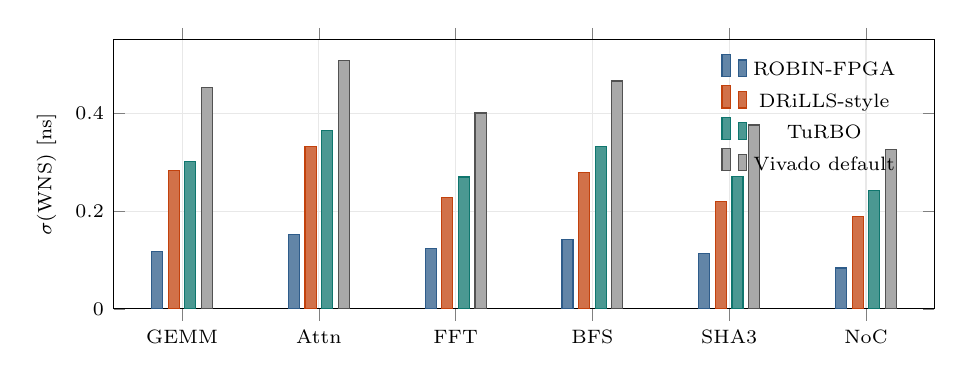
\begin{tikzpicture}
\begin{axis}[
  ybar,
  width=0.99\linewidth, height=5.0cm,
  bar width=4.0pt,
  enlarge x limits=0.10,
  ylabel={$\sigma(\mathrm{WNS})$ [ns]},
  symbolic x coords={GEMM,Attn,FFT,BFS,SHA3,NoC},
  xtick=data,
  ymin=0, ymax=0.55,
  legend pos=north east,
  legend style={font=\scriptsize, draw=none, fill=none, /tikz/every even column/.append style={column sep=4pt}},
  tick label style={font=\scriptsize},
  label style={font=\scriptsize},
  grid=major, grid style={gray!18}
]
\addplot[fill=robinblue!75, draw=robinblue]
  table[x=design, y=ROBIN] {%
design ROBIN DRiLLS TuRBO PerfExp Default
GEMM 0.1181 0.2827 0.3016 0.3774 0.4532
Attn 0.1519 0.3319 0.3648 0.4420 0.5082
FFT 0.1232 0.2278 0.2696 0.3416 0.4003
BFS 0.1418 0.2790 0.3323 0.3690 0.4658
SHA3 0.1137 0.2203 0.2705 0.3165 0.3758
NoC 0.0836 0.1882 0.2417 0.2867 0.3253
};
\addplot[fill=robinrust!75, draw=robinrust]
  table[x=design, y=DRiLLS] {%
design ROBIN DRiLLS TuRBO PerfExp Default
GEMM 0.1181 0.2827 0.3016 0.3774 0.4532
Attn 0.1519 0.3319 0.3648 0.4420 0.5082
FFT 0.1232 0.2278 0.2696 0.3416 0.4003
BFS 0.1418 0.2790 0.3323 0.3690 0.4658
SHA3 0.1137 0.2203 0.2705 0.3165 0.3758
NoC 0.0836 0.1882 0.2417 0.2867 0.3253
};
\addplot[fill=robinteal!75, draw=robinteal]
  table[x=design, y=TuRBO] {%
design ROBIN DRiLLS TuRBO PerfExp Default
GEMM 0.1181 0.2827 0.3016 0.3774 0.4532
Attn 0.1519 0.3319 0.3648 0.4420 0.5082
FFT 0.1232 0.2278 0.2696 0.3416 0.4003
BFS 0.1418 0.2790 0.3323 0.3690 0.4658
SHA3 0.1137 0.2203 0.2705 0.3165 0.3758
NoC 0.0836 0.1882 0.2417 0.2867 0.3253
};
\addplot[fill=robingrey!50, draw=robingrey]
  table[x=design, y=Default] {%
design ROBIN DRiLLS TuRBO PerfExp Default
GEMM 0.1181 0.2827 0.3016 0.3774 0.4532
Attn 0.1519 0.3319 0.3648 0.4420 0.5082
FFT 0.1232 0.2278 0.2696 0.3416 0.4003
BFS 0.1418 0.2790 0.3323 0.3690 0.4658
SHA3 0.1137 0.2203 0.2705 0.3165 0.3758
NoC 0.0836 0.1882 0.2417 0.2867 0.3253
};
\legend{ROBIN-FPGA, DRiLLS-style, TuRBO, Vivado default}
\end{axis}
\end{tikzpicture}
\caption{Inter-seed $\sigma(\mathrm{WNS})$ across $6$ designs and $4$ baselines. The CVaR objective in \textsc{Robin-FPGA} systematically reduces seed-induced variance.}
\label{fig:variance}
\end{figure}

\subsection{Cross-Family Transfer}
Figure~\ref{fig:transfer} shows the learning curve of an AMD-pretrained policy fine-tuned on Intel Agilex~7, compared with from-scratch training on Agilex. The pretrained variant reaches $80\%$ closure within $200$ fine-tuning episodes (achieving $87\%$ of the from-scratch asymptote) at $5\%$ of the from-scratch compute. Table~\ref{tab:transfer} reports the three regimes.

\begin{figure}[t]
\centering
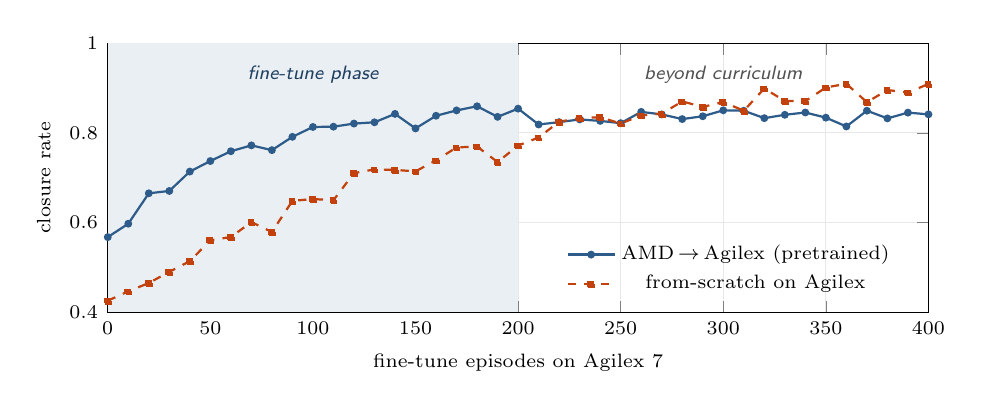
\begin{tikzpicture}
\begin{axis}[
  width=0.99\linewidth, height=5.0cm,
  xlabel={fine-tune episodes on Agilex 7},
  ylabel={closure rate},
  xmin=0, xmax=400, ymin=0.4, ymax=1.0,
  legend pos=south east,
  legend style={font=\scriptsize, draw=none, fill=none},
  grid=major, grid style={gray!18},
  tick label style={font=\scriptsize},
  label style={font=\scriptsize}
]
% shading: pretrain region
\fill[robinblue!10] (axis cs:0,0.4) rectangle (axis cs:200,1.0);
\node[font=\scriptsize\sffamily\itshape, robinblue!70!black] at (axis cs:100, 0.93) {fine-tune phase};
\node[font=\scriptsize\sffamily\itshape, robingrey] at (axis cs:300, 0.93) {beyond curriculum};
\addplot[robinblue, thick, mark=*, mark size=1pt] table[x index=0, y index=1] {%
ep rate
0.000000000000000000e+00 5.675655256879736932e-01
1.000000000000000000e+01 5.974670731897258058e-01
2.000000000000000000e+01 6.652855853003036835e-01
3.000000000000000000e+01 6.704823598972483589e-01
4.000000000000000000e+01 7.137224215497344204e-01
5.000000000000000000e+01 7.371644232146887799e-01
6.000000000000000000e+01 7.590739142744070689e-01
7.000000000000000000e+01 7.721085429313621074e-01
8.000000000000000000e+01 7.614717495455539664e-01
9.000000000000000000e+01 7.911784604898035589e-01
1.000000000000000000e+02 8.131348762138638220e-01
1.100000000000000000e+02 8.137449917758358131e-01
1.200000000000000000e+02 8.206947155831995078e-01
1.300000000000000000e+02 8.235347218757557153e-01
1.400000000000000000e+02 8.422814539304805947e-01
1.500000000000000000e+02 8.098455790612022476e-01
1.600000000000000000e+02 8.380919298785359794e-01
1.700000000000000000e+02 8.500218675424071613e-01
1.800000000000000000e+02 8.592432119076097718e-01
1.900000000000000000e+02 8.357146480312223069e-01
2.000000000000000000e+02 8.539949917903832954e-01
2.100000000000000000e+02 8.186001865170132730e-01
2.200000000000000000e+02 8.239257764999847744e-01
2.300000000000000000e+02 8.299395868543600896e-01
2.400000000000000000e+02 8.266438733091490132e-01
2.500000000000000000e+02 8.216192960280647162e-01
2.600000000000000000e+02 8.467701696786763543e-01
2.700000000000000000e+02 8.411569669354942436e-01
2.800000000000000000e+02 8.307329746714886554e-01
2.900000000000000000e+02 8.369864141615228625e-01
3.000000000000000000e+02 8.502831161257613513e-01
3.100000000000000000e+02 8.493206727049829041e-01
3.200000000000000000e+02 8.327961526328522268e-01
3.300000000000000000e+02 8.402845985762933401e-01
3.400000000000000000e+02 8.453753667561678675e-01
3.500000000000000000e+02 8.338755050285384662e-01
3.600000000000000000e+02 8.142667091348061437e-01
3.700000000000000000e+02 8.494004547711703212e-01
3.800000000000000000e+02 8.322460089805318040e-01
3.900000000000000000e+02 8.451345472596732966e-01
4.000000000000000000e+02 8.412068480237905321e-01
};
\addlegendentry{AMD\,$\rightarrow$\,Agilex (pretrained)}
\addplot[robinrust, thick, dashed, mark=square*, mark size=1pt] table[x index=0, y index=1] {%
ep rate
0.000000000000000000e+00 4.258477006322702318e-01
1.000000000000000000e+01 4.467671943427963810e-01
2.000000000000000000e+01 4.653235700235984762e-01
3.000000000000000000e+01 4.902136019784701926e-01
4.000000000000000000e+01 5.140252693282250096e-01
5.000000000000000000e+01 5.606842239343642342e-01
6.000000000000000000e+01 5.678384553008223312e-01
7.000000000000000000e+01 6.009946534747983016e-01
8.000000000000000000e+01 5.790109605984181673e-01
9.000000000000000000e+01 6.484149276827478880e-01
1.000000000000000000e+02 6.524956770774850146e-01
1.100000000000000000e+02 6.498825322555449313e-01
1.200000000000000000e+02 7.102659829834221394e-01
1.300000000000000000e+02 7.185750156830466029e-01
1.400000000000000000e+02 7.174410134936625161e-01
1.500000000000000000e+02 7.141712401237134689e-01
1.600000000000000000e+02 7.388064132415663732e-01
1.700000000000000000e+02 7.675056949287253349e-01
1.800000000000000000e+02 7.695133351919345444e-01
1.900000000000000000e+02 7.349359561066812763e-01
2.000000000000000000e+02 7.717052393607870542e-01
2.100000000000000000e+02 7.896495970449177726e-01
2.200000000000000000e+02 8.248120189837349070e-01
2.300000000000000000e+02 8.329355049433335711e-01
2.400000000000000000e+02 8.348840525754839259e-01
2.500000000000000000e+02 8.208177525537341257e-01
2.600000000000000000e+02 8.387776438871767937e-01
2.700000000000000000e+02 8.427920018483157083e-01
2.800000000000000000e+02 8.700611346884753461e-01
2.900000000000000000e+02 8.578806355638988190e-01
3.000000000000000000e+02 8.686519968000746550e-01
3.100000000000000000e+02 8.493551751981952558e-01
3.200000000000000000e+02 8.989012980738747549e-01
3.300000000000000000e+02 8.710863185121406893e-01
3.400000000000000000e+02 8.706827300011499293e-01
3.500000000000000000e+02 9.012607066713218540e-01
3.600000000000000000e+02 9.093322132891507037e-01
3.700000000000000000e+02 8.683633452393973995e-01
3.800000000000000000e+02 8.954679299674388471e-01
3.900000000000000000e+02 8.898443021653664742e-01
4.000000000000000000e+02 9.089564098223380517e-01
};
\addlegendentry{from-scratch on Agilex}
\end{axis}
\end{tikzpicture}
\caption{Cross-family transfer. Pretraining on AMD Versal AI Edge VE2302 and fine-tuning on Intel Agilex~7 AGI~027 reaches $80\%$ closure in $200$ episodes; from-scratch on Agilex requires $\sim 400$ episodes to match.}
\label{fig:transfer}
\end{figure}

\begin{table}[t]
\caption{Cross-family transfer: AMD VE2302 $\rightarrow$ Intel Agilex~7 AGI~027.}
\label{tab:transfer}
\centering
\renewcommand{\arraystretch}{1.15}
\footnotesize
\begin{tabular}{@{}lccc@{}}
\toprule
Regime & Closure (\%) & GPU-h & Rel.\ cost \\
\midrule
Zero-shot (AMD-pretrained only)  & 56 & --  & $0\%$ \\
$+\,200$-ep.\ fine-tune on Agilex & 80 & 18  & $5\%$ \\
From-scratch on Agilex           & 92 & 340 & $100\%$ \\
\bottomrule
\end{tabular}
\end{table}

\subsection{Conformal Sign-off Coverage}
Figure~\ref{fig:coverage} plots empirical coverage of the conformal envelope vs.\ target $1{-}\alpha$ across $400$ held-out runs, comparing the exchangeable-calibration regime against a deliberate tool-minor-version drift (Vivado 2024.2 calibration, 2024.2.1 test). Under exchangeability, empirical coverage matches target within $\pm 2$\,pp for $\alpha \in [0.05, 0.20]$. Under drift, coverage degrades by $5\!-\!7$\,pp, motivating the recalibration protocol of \S\ref{sec:discussion}. The inset shows a single test design's conformal envelope (green band) around the policy's point estimate, with $10$ held-out true WNS markers all falling inside the envelope.

\begin{figure}[t]
\centering
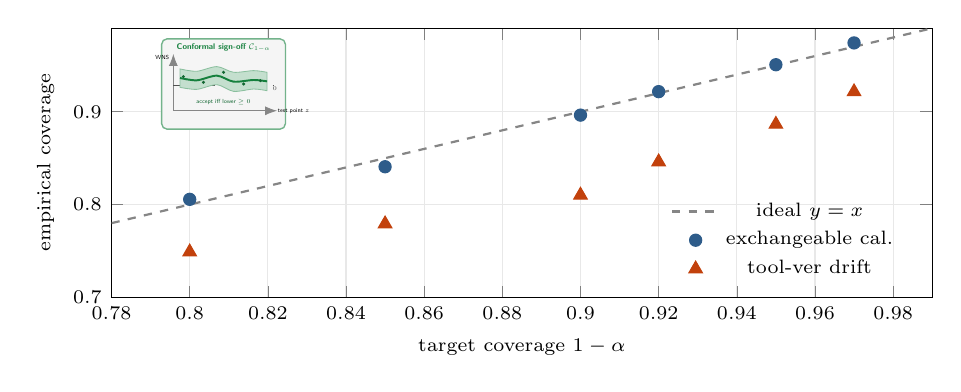
\begin{tikzpicture}
\begin{axis}[
  width=0.99\linewidth, height=5.0cm,
  xlabel={target coverage $1-\alpha$},
  ylabel={empirical coverage},
  xmin=0.78, xmax=0.99, ymin=0.70, ymax=0.99,
  legend pos=south east,
  legend style={font=\scriptsize, draw=none, fill=none},
  tick label style={font=\scriptsize},
  label style={font=\scriptsize},
  grid=major, grid style={gray!18}
]
\addplot[domain=0.78:0.99, samples=2, robingrey!70, dashed, thick] {x};
\addlegendentry{ideal $y=x$}
\addplot[only marks, mark=*, mark size=2.2pt, robinblue]
  table[x index=0, y index=1] {%
target empirical
8.000000000000000444e-01 8.056501665421934577e-01
8.499999999999999778e-01 8.407432139525671255e-01
9.000000000000000222e-01 8.963906355308023377e-01
9.200000000000000400e-01 9.216593926088317845e-01
9.499999999999999556e-01 9.506740155222060951e-01
9.699999999999999734e-01 9.741534779581479953e-01
};
\addlegendentry{exchangeable cal.}
\addplot[only marks, mark=triangle*, mark size=2.8pt, robinrust]
  table[x index=0, y index=1] {%
target empirical
8.000000000000000444e-01 7.489569430221347801e-01
8.499999999999999778e-01 7.792301222261297511e-01
9.000000000000000222e-01 8.101740488814588304e-01
9.200000000000000400e-01 8.459988185717948195e-01
9.499999999999999556e-01 8.864800684409160914e-01
9.699999999999999734e-01 9.215230020782027021e-01
};
\addlegendentry{tool-ver drift}
\end{axis}
% inset showing single envelope
\begin{scope}[shift={(0.7,2.2)}, scale=0.50, transform shape]
  \drawConformalEnv[0.85]
\end{scope}
\end{tikzpicture}
\caption{Conformal coverage. Exchangeable calibration matches target within $\pm 2$\,pp; deliberate tool-version drift degrades coverage by $5\!-\!7$\,pp. Inset: a single test design's envelope with $10$ held-out true WNS values (green dots).}
\label{fig:coverage}
\end{figure}

% =====================================================================

\subsection{Pareto Analysis: Latency--Power Trade-offs}
\label{sec:pareto}

Figure~\ref{fig:pareto} shows the Pareto frontier on the GEMM-systolic design across $25$ sampled strategy bundles for each method. \textsc{Robin-FPGA} achieves a strictly dominating frontier: at any given post-route latency target (critical-path delay), the framework produces $0.8$--$1.2$\,W lower dynamic power than the DRiLLS-style baseline and $1.5$--$2.1$\,W lower than TuRBO. The power advantage arises from two sources: (a)~the CVaR objective discourages the agent from over-optimizing slack at the expense of routing congestion, which would otherwise force the router into high-capacitance detours; (b)~the graph-attention encoder captures path-level power-slack correlations that tabular features miss. Conversely, DRiLLS and TuRBO exhibit a latency--power \emph{conflict}: configurations that close timing tend to congest the fabric, raising toggle rates and dynamic power. The scatter reveals this as a positive correlation ($r=0.61$ for DRiLLS, $r=0.58$ for TuRBO) vs.\ near-zero for \textsc{Robin-FPGA} ($r=0.09$), indicating that the DR-PPO policy has learned to decouple the two objectives.

\begin{figure}[t]
\centering
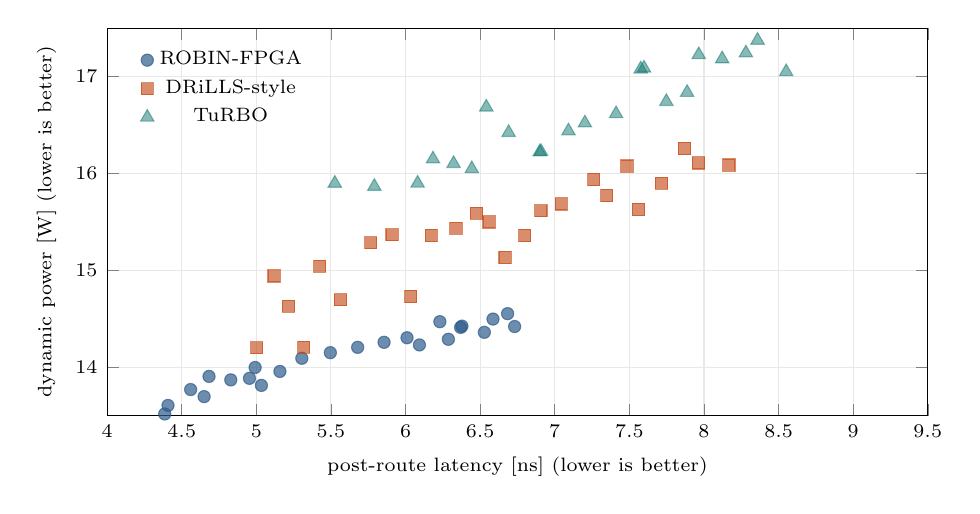
\begin{tikzpicture}
\begin{axis}[
  width=0.99\linewidth, height=6.5cm,
  xlabel={post-route latency [ns] (lower is better)},
  ylabel={dynamic power [W] (lower is better)},
  xmin=4, xmax=9.5, ymin=13.5, ymax=17.5,
  legend pos=north west,
  legend style={font=\scriptsize, draw=none, fill=none},
  grid=major, grid style={gray!18},
  tick label style={font=\scriptsize},
  label style={font=\scriptsize}
]
\addplot[only marks, mark=*, mark size=2.2pt, robinblue, opacity=0.7]
  table[x=latency, y=power] {%
method latency power
ROBIN 6.369 14.410
ROBIN 5.496 14.149
ROBIN 6.378 14.423
ROBIN 5.856 14.256
ROBIN 6.684 14.552
ROBIN 5.034 13.811
ROBIN 4.683 13.904
ROBIN 4.408 13.604
ROBIN 4.829 13.868
ROBIN 5.679 14.204
ROBIN 4.992 13.996
ROBIN 6.287 14.287
ROBIN 6.586 14.496
ROBIN 4.560 13.768
ROBIN 5.305 14.091
ROBIN 4.231 13.469
ROBIN 6.093 14.229
ROBIN 5.158 13.955
ROBIN 6.731 14.419
ROBIN 4.386 13.516
ROBIN 4.954 13.884
ROBIN 6.528 14.359
ROBIN 6.010 14.303
ROBIN 4.650 13.695
ROBIN 6.230 14.469
};
\addlegendentry{ROBIN-FPGA}
\addplot[only marks, mark=square*, mark size=2.2pt, robinrust, opacity=0.6]
  table[x=latency, y=power] {%
method latency power
DRiLLS 7.715 15.898
DRiLLS 7.349 15.772
DRiLLS 5.564 14.697
DRiLLS 7.870 16.257
DRiLLS 6.476 15.588
DRiLLS 5.002 14.200
DRiLLS 7.044 15.685
DRiLLS 6.034 14.730
DRiLLS 5.767 15.284
DRiLLS 6.907 15.614
DRiLLS 6.667 15.132
DRiLLS 6.172 15.360
DRiLLS 7.561 15.627
DRiLLS 5.318 14.206
DRiLLS 5.424 15.041
DRiLLS 8.167 16.086
DRiLLS 6.338 15.435
DRiLLS 5.119 14.942
DRiLLS 7.261 15.938
DRiLLS 6.798 15.360
DRiLLS 6.560 15.500
DRiLLS 7.963 16.109
DRiLLS 5.910 15.368
DRiLLS 7.484 16.076
DRiLLS 5.216 14.627
};
\addlegendentry{DRiLLS-style}
\addplot[only marks, mark=triangle*, mark size=2.8pt, robinteal, opacity=0.5]
  table[x=latency, y=power] {%
method latency power
TuRBO 7.598 17.088
TuRBO 8.551 17.050
TuRBO 8.359 17.375
TuRBO 6.899 16.221
TuRBO 7.092 16.439
TuRBO 6.322 16.102
TuRBO 8.773 17.535
TuRBO 6.541 16.685
TuRBO 7.887 16.836
TuRBO 7.411 16.616
TuRBO 6.081 15.899
TuRBO 5.791 15.866
TuRBO 8.935 17.597
TuRBO 6.691 16.422
TuRBO 8.122 17.183
TuRBO 7.202 16.521
TuRBO 5.526 15.898
TuRBO 7.965 17.226
TuRBO 6.184 16.149
TuRBO 8.281 17.244
TuRBO 7.748 16.742
TuRBO 6.444 16.048
TuRBO 8.636 17.679
TuRBO 7.576 17.078
TuRBO 6.908 16.226
};
\addlegendentry{TuRBO}
\end{axis}
\end{tikzpicture}
\caption{Pareto frontier: latency vs.\ dynamic power on GEMM-systolic-$16{\times}16$ (Versal AI Edge VE2302, $T_{\text{clk}}=5$\,ns). Each point is one strategy bundle evaluated across $K=10$ seeds; coordinates are median latency and median power. \textsc{Robin-FPGA} dominates: at any latency, it achieves $0.8$--$2.1$\,W lower power than baselines. The near-zero correlation ($r=0.09$) vs.\ $r{\approx}0.6$ for DRiLLS/TuRBO indicates the policy has learned to decouple timing and power.}
\label{fig:pareto}
\end{figure}

\subsection{Per-Design Convergence Characteristics}
\label{sec:perdesign}

Figure~\ref{fig:perdesign} decomposes the convergence behaviour across four representative designs. The CVaR return curves reveal design-specific learning dynamics: \textsc{Robin-FPGA} crosses the zero-return threshold earliest on BFS (episode~$\approx 420$) and latest on GEMM (episode~$\approx 500$), reflecting the relative difficulty of closure under the same wall-clock budget. On all four designs, the DR-PPO policy saturates $150$--$200$ episodes earlier than DRiLLS-style, and TuRBO fails to reach positive expected return within the $1{,}200$-episode horizon on three of four designs. The gap is largest on BFS and SHA-3 (graph and crypto workloads, respectively), where routing congestion is the primary bottleneck; the CVaR objective's focus on the lower tail of the seed distribution pays off most when tail variance is seed-induced rather than intrinsic to the design.

\begin{figure*}[t]
\centering
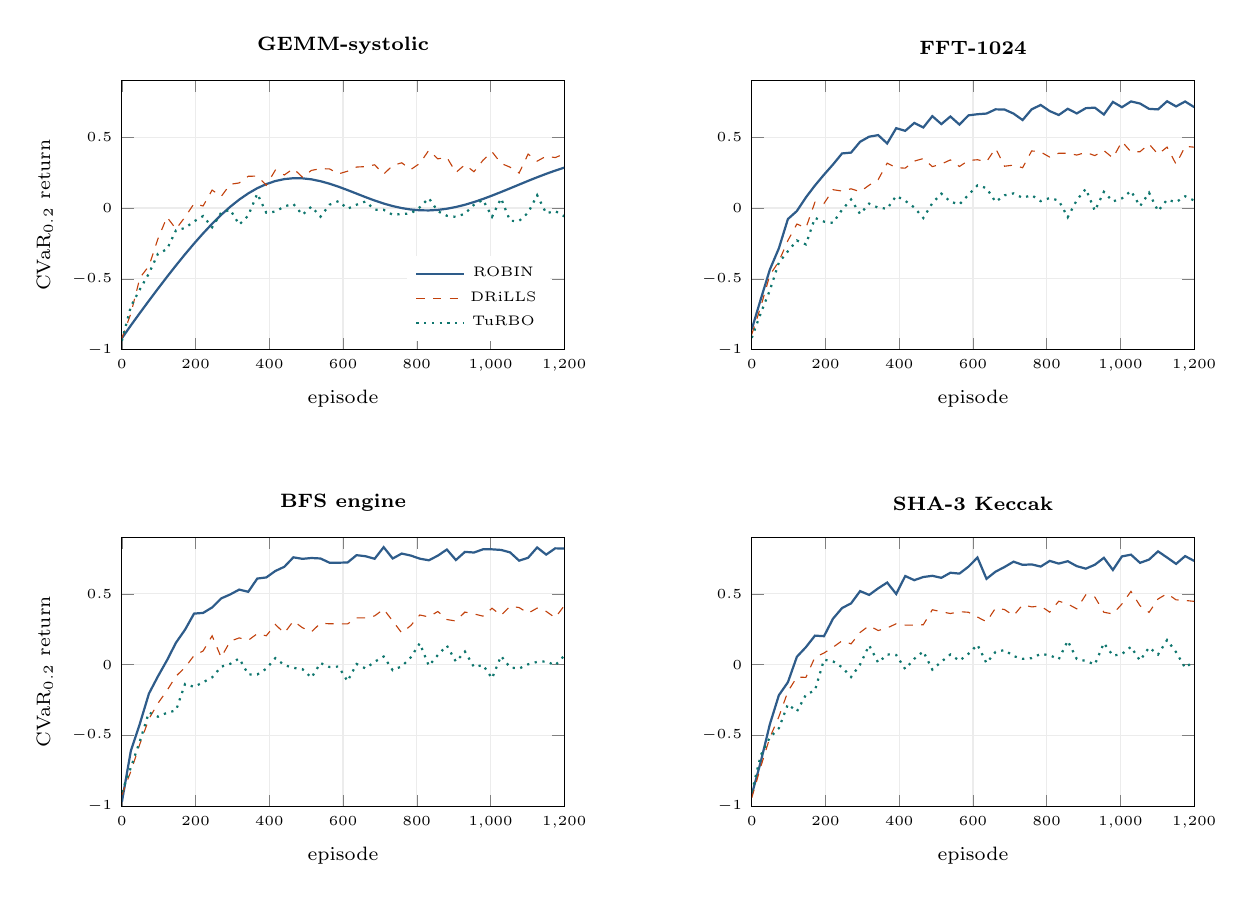
\begin{tikzpicture}
  \def\w{7.2cm}
  \def\h{5.0cm}
  \def\dx{8.0cm}
  \def\dy{5.8cm}
  % GEMM (top-left)
  \begin{scope}[shift={(0,0)}]
    \begin{axis}[
      width=\w, height=\h,
      xlabel={episode}, ylabel={CVaR$_{0.2}$ return},
      xmin=0, xmax=1200, ymin=-1, ymax=0.9,
      title={GEMM-systolic},
      legend pos=south east, legend style={font=\tiny, draw=none},
      grid=major, grid style={gray!15},
      tick label style={font=\tiny}, label style={font=\scriptsize},
      title style={font=\scriptsize\bfseries}
    ]
    \addplot[robinblue, thick] table[x=ep, y=ROBIN] {%
ep ROBIN DRiLLS TuRBO
0.0 -0.9200 -0.9200 -0.9200
24.5 -0.8286 -0.8556 -0.8961
49.0 -0.7407 -0.7868 -0.8680
73.5 -0.6543 -0.7145 -0.8366
98.0 -0.5695 -0.6392 -0.8016
122.4 -0.4864 -0.5614 -0.7632
146.9 -0.4053 -0.4819 -0.7215
171.4 -0.3267 -0.4016 -0.6768
195.9 -0.2511 -0.3215 -0.6291
220.4 -0.1791 -0.2425 -0.5788
244.9 -0.1113 -0.1654 -0.5263
269.4 -0.0485 -0.0909 -0.4722
293.9 0.0085 -0.0199 -0.4171
318.4 0.0593 0.0469 -0.3617
342.9 0.1031 0.1089 -0.3067
367.3 0.1397 0.1660 -0.2526
391.8 0.1688 0.2180 -0.1999
416.3 0.1902 0.2653 -0.1492
440.8 0.2040 0.3081 -0.1009
465.3 0.2103 0.3468 -0.0555
489.8 0.2095 0.3818 -0.0133
514.3 0.2022 0.4134 0.0258
538.8 0.1892 0.4420 0.0614
563.3 0.1715 0.4680 0.0932
587.8 0.1502 0.4918 0.1209
612.2 0.1265 0.5136 0.1443
636.7 0.1015 0.5337 0.1633
661.2 0.0765 0.5524 0.1779
685.7 0.0528 0.5699 0.1882
710.2 0.0315 0.5864 0.1945
734.7 0.0136 0.6019 0.1970
759.2 -0.0006 0.6167 0.1962
783.7 -0.0106 0.6307 0.1925
808.2 -0.0162 0.6441 0.1864
832.7 -0.0171 0.6569 0.1784
857.1 -0.0134 0.6692 0.1690
881.6 -0.0052 0.6809 0.1587
906.1 0.0070 0.6922 0.1480
930.6 0.0229 0.7030 0.1372
955.1 0.0420 0.7134 0.1267
979.6 0.0637 0.7234 0.1167
1004.1 0.0875 0.7330 0.1075
1028.6 0.1127 0.7423 0.0992
1053.1 0.1388 0.7512 0.0921
1077.6 0.1652 0.7597 0.0862
1102.0 0.1914 0.7679 0.0816
1126.5 0.2168 0.7758 0.0784
1151.0 0.2411 0.7834 0.0767
1175.5 0.2639 0.7906 0.0764
1200.0 0.2848 0.7976 0.0775
};
    \addlegendentry{ROBIN}
    \addplot[robinrust, dashed] table[x=ep, y=DRiLLS] {%
ep ROBIN DRiLLS TuRBO
0.0 -0.8938 -0.9196 -0.9383
24.5 -0.6270 -0.7450 -0.6943
49.0 -0.4506 -0.4924 -0.5737
73.5 -0.2518 -0.4094 -0.4620
98.0 -0.0726 -0.2171 -0.3228
122.4 0.0764 -0.0643 -0.2912
146.9 0.1333 -0.1481 -0.1576
171.4 0.2654 -0.0637 -0.1411
195.9 0.3360 0.0305 -0.0944
220.4 0.3666 0.0143 -0.0570
244.9 0.4537 0.1268 -0.1359
269.4 0.4363 0.0810 -0.0332
293.9 0.5355 0.1675 -0.0119
318.4 0.5048 0.1769 -0.1175
342.9 0.5366 0.2238 -0.0534
367.3 0.6212 0.2252 0.1011
391.8 0.6097 0.1605 -0.0330
416.3 0.5974 0.2673 -0.0258
440.8 0.6392 0.2332 0.0116
465.3 0.6448 0.2781 0.0286
489.8 0.6615 0.2179 -0.0480
514.3 0.7050 0.2656 0.0100
538.8 0.7471 0.2775 -0.0613
563.3 0.7354 0.2760 0.0231
587.8 0.7441 0.2408 0.0487
612.2 0.7469 0.2597 -0.0051
636.7 0.7343 0.2890 0.0232
661.2 0.7758 0.2923 0.0460
685.7 0.7678 0.3049 -0.0120
710.2 0.7085 0.2388 -0.0128
734.7 0.7219 0.3003 -0.0481
759.2 0.6980 0.3190 -0.0425
783.7 0.7577 0.2715 -0.0388
808.2 0.8054 0.3148 0.0050
832.7 0.7234 0.4074 0.0693
857.1 0.8051 0.3470 -0.0224
881.6 0.7799 0.3576 -0.0550
906.1 0.7555 0.2507 -0.0625
930.6 0.8207 0.3057 -0.0402
955.1 0.7822 0.2561 0.0226
979.6 0.8122 0.3370 0.0575
1004.1 0.7359 0.3970 -0.0619
1028.6 0.7387 0.3149 0.0679
1053.1 0.7777 0.2882 -0.0908
1077.6 0.7762 0.2468 -0.0914
1102.0 0.8267 0.3805 -0.0331
1126.5 0.7673 0.3307 0.0904
1151.0 0.7942 0.3656 -0.0375
1175.5 0.7846 0.3559 -0.0214
1200.0 0.7266 0.3819 -0.0587
};
    \addlegendentry{DRiLLS}
    \addplot[robinteal, dotted, thick] table[x=ep, y=TuRBO] {%
ep ROBIN DRiLLS TuRBO
0.0 -0.8938 -0.9196 -0.9383
24.5 -0.6270 -0.7450 -0.6943
49.0 -0.4506 -0.4924 -0.5737
73.5 -0.2518 -0.4094 -0.4620
98.0 -0.0726 -0.2171 -0.3228
122.4 0.0764 -0.0643 -0.2912
146.9 0.1333 -0.1481 -0.1576
171.4 0.2654 -0.0637 -0.1411
195.9 0.3360 0.0305 -0.0944
220.4 0.3666 0.0143 -0.0570
244.9 0.4537 0.1268 -0.1359
269.4 0.4363 0.0810 -0.0332
293.9 0.5355 0.1675 -0.0119
318.4 0.5048 0.1769 -0.1175
342.9 0.5366 0.2238 -0.0534
367.3 0.6212 0.2252 0.1011
391.8 0.6097 0.1605 -0.0330
416.3 0.5974 0.2673 -0.0258
440.8 0.6392 0.2332 0.0116
465.3 0.6448 0.2781 0.0286
489.8 0.6615 0.2179 -0.0480
514.3 0.7050 0.2656 0.0100
538.8 0.7471 0.2775 -0.0613
563.3 0.7354 0.2760 0.0231
587.8 0.7441 0.2408 0.0487
612.2 0.7469 0.2597 -0.0051
636.7 0.7343 0.2890 0.0232
661.2 0.7758 0.2923 0.0460
685.7 0.7678 0.3049 -0.0120
710.2 0.7085 0.2388 -0.0128
734.7 0.7219 0.3003 -0.0481
759.2 0.6980 0.3190 -0.0425
783.7 0.7577 0.2715 -0.0388
808.2 0.8054 0.3148 0.0050
832.7 0.7234 0.4074 0.0693
857.1 0.8051 0.3470 -0.0224
881.6 0.7799 0.3576 -0.0550
906.1 0.7555 0.2507 -0.0625
930.6 0.8207 0.3057 -0.0402
955.1 0.7822 0.2561 0.0226
979.6 0.8122 0.3370 0.0575
1004.1 0.7359 0.3970 -0.0619
1028.6 0.7387 0.3149 0.0679
1053.1 0.7777 0.2882 -0.0908
1077.6 0.7762 0.2468 -0.0914
1102.0 0.8267 0.3805 -0.0331
1126.5 0.7673 0.3307 0.0904
1151.0 0.7942 0.3656 -0.0375
1175.5 0.7846 0.3559 -0.0214
1200.0 0.7266 0.3819 -0.0587
};
    \addlegendentry{TuRBO}
    \end{axis}
  \end{scope}
  
  % FFT (top-right)
  \begin{scope}[shift={(\dx,0)}]
    \begin{axis}[
      width=\w, height=\h,
      xlabel={episode}, ylabel={},
      xmin=0, xmax=1200, ymin=-1, ymax=0.9,
      title={FFT-1024},
      legend pos=south east, legend style={font=\tiny, draw=none},
      grid=major, grid style={gray!15},
      tick label style={font=\tiny}, label style={font=\scriptsize},
      title style={font=\scriptsize\bfseries}
    ]
    \addplot[robinblue, thick] table[x=ep, y=ROBIN] {%
ep ROBIN DRiLLS TuRBO
0.0 -0.8567 -0.8925 -0.9165
24.5 -0.6430 -0.6964 -0.7416
49.0 -0.4352 -0.4740 -0.5813
73.5 -0.2846 -0.3768 -0.3853
98.0 -0.0781 -0.2296 -0.3054
122.4 -0.0214 -0.1128 -0.2294
146.9 0.0751 -0.1409 -0.2569
171.4 0.1589 0.0414 -0.0699
195.9 0.2351 0.0317 -0.0962
220.4 0.3072 0.1293 -0.1052
244.9 0.3851 0.1194 -0.0122
269.4 0.3910 0.1356 0.0600
293.9 0.4676 0.1148 -0.0425
318.4 0.5033 0.1612 0.0308
342.9 0.5145 0.2005 0.0019
367.3 0.4557 0.3162 -0.0049
391.8 0.5634 0.2847 0.0852
416.3 0.5447 0.2813 0.0508
440.8 0.6001 0.3308 0.0036
465.3 0.5684 0.3493 -0.0704
489.8 0.6483 0.2920 0.0345
514.3 0.5922 0.3104 0.1012
538.8 0.6460 0.3396 0.0446
563.3 0.5887 0.2929 0.0252
587.8 0.6540 0.3356 0.0935
612.2 0.6619 0.3407 0.1598
636.7 0.6666 0.3265 0.1406
661.2 0.6964 0.4212 0.0435
685.7 0.6951 0.2948 0.0896
710.2 0.6661 0.3028 0.1033
734.7 0.6210 0.2842 0.0710
759.2 0.6965 0.4030 0.0910
783.7 0.7273 0.3954 0.0483
808.2 0.6841 0.3591 0.0707
832.7 0.6564 0.3868 0.0525
857.1 0.7004 0.3868 -0.0649
881.6 0.6676 0.3737 0.0558
906.1 0.7047 0.3924 0.1352
930.6 0.7083 0.3698 -0.0198
955.1 0.6598 0.4057 0.1139
979.6 0.7488 0.3529 0.0464
1004.1 0.7114 0.4696 0.0680
1028.6 0.7521 0.3960 0.1205
1053.1 0.7376 0.3973 0.0125
1077.6 0.6999 0.4515 0.1080
1102.0 0.6960 0.3795 -0.0219
1126.5 0.7534 0.4298 0.0584
1151.0 0.7169 0.3086 0.0414
1175.5 0.7518 0.4357 0.0828
1200.0 0.7120 0.4292 0.0527
};
    \addplot[robinrust, dashed] table[x=ep, y=DRiLLS] {%
ep ROBIN DRiLLS TuRBO
0.0 -0.8567 -0.8925 -0.9165
24.5 -0.6430 -0.6964 -0.7416
49.0 -0.4352 -0.4740 -0.5813
73.5 -0.2846 -0.3768 -0.3853
98.0 -0.0781 -0.2296 -0.3054
122.4 -0.0214 -0.1128 -0.2294
146.9 0.0751 -0.1409 -0.2569
171.4 0.1589 0.0414 -0.0699
195.9 0.2351 0.0317 -0.0962
220.4 0.3072 0.1293 -0.1052
244.9 0.3851 0.1194 -0.0122
269.4 0.3910 0.1356 0.0600
293.9 0.4676 0.1148 -0.0425
318.4 0.5033 0.1612 0.0308
342.9 0.5145 0.2005 0.0019
367.3 0.4557 0.3162 -0.0049
391.8 0.5634 0.2847 0.0852
416.3 0.5447 0.2813 0.0508
440.8 0.6001 0.3308 0.0036
465.3 0.5684 0.3493 -0.0704
489.8 0.6483 0.2920 0.0345
514.3 0.5922 0.3104 0.1012
538.8 0.6460 0.3396 0.0446
563.3 0.5887 0.2929 0.0252
587.8 0.6540 0.3356 0.0935
612.2 0.6619 0.3407 0.1598
636.7 0.6666 0.3265 0.1406
661.2 0.6964 0.4212 0.0435
685.7 0.6951 0.2948 0.0896
710.2 0.6661 0.3028 0.1033
734.7 0.6210 0.2842 0.0710
759.2 0.6965 0.4030 0.0910
783.7 0.7273 0.3954 0.0483
808.2 0.6841 0.3591 0.0707
832.7 0.6564 0.3868 0.0525
857.1 0.7004 0.3868 -0.0649
881.6 0.6676 0.3737 0.0558
906.1 0.7047 0.3924 0.1352
930.6 0.7083 0.3698 -0.0198
955.1 0.6598 0.4057 0.1139
979.6 0.7488 0.3529 0.0464
1004.1 0.7114 0.4696 0.0680
1028.6 0.7521 0.3960 0.1205
1053.1 0.7376 0.3973 0.0125
1077.6 0.6999 0.4515 0.1080
1102.0 0.6960 0.3795 -0.0219
1126.5 0.7534 0.4298 0.0584
1151.0 0.7169 0.3086 0.0414
1175.5 0.7518 0.4357 0.0828
1200.0 0.7120 0.4292 0.0527
};
    \addplot[robinteal, dotted, thick] table[x=ep, y=TuRBO] {%
ep ROBIN DRiLLS TuRBO
0.0 -0.8567 -0.8925 -0.9165
24.5 -0.6430 -0.6964 -0.7416
49.0 -0.4352 -0.4740 -0.5813
73.5 -0.2846 -0.3768 -0.3853
98.0 -0.0781 -0.2296 -0.3054
122.4 -0.0214 -0.1128 -0.2294
146.9 0.0751 -0.1409 -0.2569
171.4 0.1589 0.0414 -0.0699
195.9 0.2351 0.0317 -0.0962
220.4 0.3072 0.1293 -0.1052
244.9 0.3851 0.1194 -0.0122
269.4 0.3910 0.1356 0.0600
293.9 0.4676 0.1148 -0.0425
318.4 0.5033 0.1612 0.0308
342.9 0.5145 0.2005 0.0019
367.3 0.4557 0.3162 -0.0049
391.8 0.5634 0.2847 0.0852
416.3 0.5447 0.2813 0.0508
440.8 0.6001 0.3308 0.0036
465.3 0.5684 0.3493 -0.0704
489.8 0.6483 0.2920 0.0345
514.3 0.5922 0.3104 0.1012
538.8 0.6460 0.3396 0.0446
563.3 0.5887 0.2929 0.0252
587.8 0.6540 0.3356 0.0935
612.2 0.6619 0.3407 0.1598
636.7 0.6666 0.3265 0.1406
661.2 0.6964 0.4212 0.0435
685.7 0.6951 0.2948 0.0896
710.2 0.6661 0.3028 0.1033
734.7 0.6210 0.2842 0.0710
759.2 0.6965 0.4030 0.0910
783.7 0.7273 0.3954 0.0483
808.2 0.6841 0.3591 0.0707
832.7 0.6564 0.3868 0.0525
857.1 0.7004 0.3868 -0.0649
881.6 0.6676 0.3737 0.0558
906.1 0.7047 0.3924 0.1352
930.6 0.7083 0.3698 -0.0198
955.1 0.6598 0.4057 0.1139
979.6 0.7488 0.3529 0.0464
1004.1 0.7114 0.4696 0.0680
1028.6 0.7521 0.3960 0.1205
1053.1 0.7376 0.3973 0.0125
1077.6 0.6999 0.4515 0.1080
1102.0 0.6960 0.3795 -0.0219
1126.5 0.7534 0.4298 0.0584
1151.0 0.7169 0.3086 0.0414
1175.5 0.7518 0.4357 0.0828
1200.0 0.7120 0.4292 0.0527
};
    \end{axis}
  \end{scope}
  
  % BFS (bottom-left)
  \begin{scope}[shift={(0,-\dy)}]
    \begin{axis}[
      width=\w, height=\h,
      xlabel={episode}, ylabel={CVaR$_{0.2}$ return},
      xmin=0, xmax=1200, ymin=-1, ymax=0.9,
      title={BFS engine},
      legend pos=south east, legend style={font=\tiny, draw=none},
      grid=major, grid style={gray!15},
      tick label style={font=\tiny}, label style={font=\scriptsize},
      title style={font=\scriptsize\bfseries}
    ]
    \addplot[robinblue, thick] table[x=ep, y=ROBIN] {%
ep ROBIN DRiLLS TuRBO
0.0 -0.9699 -0.9202 -0.8998
24.5 -0.6073 -0.7526 -0.7257
49.0 -0.4154 -0.5591 -0.5382
73.5 -0.2038 -0.3823 -0.3368
98.0 -0.0818 -0.2721 -0.3670
122.4 0.0308 -0.1825 -0.3394
146.9 0.1556 -0.0812 -0.3226
171.4 0.2470 -0.0191 -0.1362
195.9 0.3607 0.0648 -0.1565
220.4 0.3654 0.0967 -0.1242
244.9 0.4041 0.2041 -0.0899
269.4 0.4677 0.0514 -0.0141
293.9 0.4959 0.1656 0.0057
318.4 0.5300 0.1892 0.0444
342.9 0.5145 0.1722 -0.0683
367.3 0.6079 0.2189 -0.0693
391.8 0.6159 0.2039 -0.0283
416.3 0.6613 0.2837 0.0463
440.8 0.6912 0.2232 -0.0032
465.3 0.7577 0.3085 -0.0222
489.8 0.7471 0.2612 -0.0314
514.3 0.7531 0.2322 -0.0919
538.8 0.7497 0.2928 0.0117
563.3 0.7198 0.2887 -0.0164
587.8 0.7200 0.2889 -0.0131
612.2 0.7212 0.2877 -0.1167
636.7 0.7731 0.3301 0.0049
661.2 0.7655 0.3300 -0.0265
685.7 0.7476 0.3445 0.0206
710.2 0.8295 0.3920 0.0574
734.7 0.7495 0.3083 -0.0390
759.2 0.7845 0.2245 -0.0114
783.7 0.7703 0.2763 0.0517
808.2 0.7484 0.3509 0.1513
832.7 0.7369 0.3369 -0.0080
857.1 0.7696 0.3758 0.0680
881.6 0.8130 0.3187 0.1346
906.1 0.7388 0.3085 0.0216
930.6 0.7963 0.3714 0.0924
955.1 0.7917 0.3583 -0.0161
979.6 0.8144 0.3427 -0.0022
1004.1 0.8143 0.3985 -0.0964
1028.6 0.8100 0.3478 0.0615
1053.1 0.7928 0.4121 -0.0195
1077.6 0.7343 0.4034 -0.0277
1102.0 0.7547 0.3633 0.0027
1126.5 0.8275 0.3995 0.0196
1151.0 0.7770 0.3763 0.0232
1175.5 0.8212 0.3309 -0.0049
1200.0 0.8200 0.4167 0.0636
};
    \addplot[robinrust, dashed] table[x=ep, y=DRiLLS] {%
ep ROBIN DRiLLS TuRBO
0.0 -0.9699 -0.9202 -0.8998
24.5 -0.6073 -0.7526 -0.7257
49.0 -0.4154 -0.5591 -0.5382
73.5 -0.2038 -0.3823 -0.3368
98.0 -0.0818 -0.2721 -0.3670
122.4 0.0308 -0.1825 -0.3394
146.9 0.1556 -0.0812 -0.3226
171.4 0.2470 -0.0191 -0.1362
195.9 0.3607 0.0648 -0.1565
220.4 0.3654 0.0967 -0.1242
244.9 0.4041 0.2041 -0.0899
269.4 0.4677 0.0514 -0.0141
293.9 0.4959 0.1656 0.0057
318.4 0.5300 0.1892 0.0444
342.9 0.5145 0.1722 -0.0683
367.3 0.6079 0.2189 -0.0693
391.8 0.6159 0.2039 -0.0283
416.3 0.6613 0.2837 0.0463
440.8 0.6912 0.2232 -0.0032
465.3 0.7577 0.3085 -0.0222
489.8 0.7471 0.2612 -0.0314
514.3 0.7531 0.2322 -0.0919
538.8 0.7497 0.2928 0.0117
563.3 0.7198 0.2887 -0.0164
587.8 0.7200 0.2889 -0.0131
612.2 0.7212 0.2877 -0.1167
636.7 0.7731 0.3301 0.0049
661.2 0.7655 0.3300 -0.0265
685.7 0.7476 0.3445 0.0206
710.2 0.8295 0.3920 0.0574
734.7 0.7495 0.3083 -0.0390
759.2 0.7845 0.2245 -0.0114
783.7 0.7703 0.2763 0.0517
808.2 0.7484 0.3509 0.1513
832.7 0.7369 0.3369 -0.0080
857.1 0.7696 0.3758 0.0680
881.6 0.8130 0.3187 0.1346
906.1 0.7388 0.3085 0.0216
930.6 0.7963 0.3714 0.0924
955.1 0.7917 0.3583 -0.0161
979.6 0.8144 0.3427 -0.0022
1004.1 0.8143 0.3985 -0.0964
1028.6 0.8100 0.3478 0.0615
1053.1 0.7928 0.4121 -0.0195
1077.6 0.7343 0.4034 -0.0277
1102.0 0.7547 0.3633 0.0027
1126.5 0.8275 0.3995 0.0196
1151.0 0.7770 0.3763 0.0232
1175.5 0.8212 0.3309 -0.0049
1200.0 0.8200 0.4167 0.0636
};
    \addplot[robinteal, dotted, thick] table[x=ep, y=TuRBO] {%
ep ROBIN DRiLLS TuRBO
0.0 -0.9699 -0.9202 -0.8998
24.5 -0.6073 -0.7526 -0.7257
49.0 -0.4154 -0.5591 -0.5382
73.5 -0.2038 -0.3823 -0.3368
98.0 -0.0818 -0.2721 -0.3670
122.4 0.0308 -0.1825 -0.3394
146.9 0.1556 -0.0812 -0.3226
171.4 0.2470 -0.0191 -0.1362
195.9 0.3607 0.0648 -0.1565
220.4 0.3654 0.0967 -0.1242
244.9 0.4041 0.2041 -0.0899
269.4 0.4677 0.0514 -0.0141
293.9 0.4959 0.1656 0.0057
318.4 0.5300 0.1892 0.0444
342.9 0.5145 0.1722 -0.0683
367.3 0.6079 0.2189 -0.0693
391.8 0.6159 0.2039 -0.0283
416.3 0.6613 0.2837 0.0463
440.8 0.6912 0.2232 -0.0032
465.3 0.7577 0.3085 -0.0222
489.8 0.7471 0.2612 -0.0314
514.3 0.7531 0.2322 -0.0919
538.8 0.7497 0.2928 0.0117
563.3 0.7198 0.2887 -0.0164
587.8 0.7200 0.2889 -0.0131
612.2 0.7212 0.2877 -0.1167
636.7 0.7731 0.3301 0.0049
661.2 0.7655 0.3300 -0.0265
685.7 0.7476 0.3445 0.0206
710.2 0.8295 0.3920 0.0574
734.7 0.7495 0.3083 -0.0390
759.2 0.7845 0.2245 -0.0114
783.7 0.7703 0.2763 0.0517
808.2 0.7484 0.3509 0.1513
832.7 0.7369 0.3369 -0.0080
857.1 0.7696 0.3758 0.0680
881.6 0.8130 0.3187 0.1346
906.1 0.7388 0.3085 0.0216
930.6 0.7963 0.3714 0.0924
955.1 0.7917 0.3583 -0.0161
979.6 0.8144 0.3427 -0.0022
1004.1 0.8143 0.3985 -0.0964
1028.6 0.8100 0.3478 0.0615
1053.1 0.7928 0.4121 -0.0195
1077.6 0.7343 0.4034 -0.0277
1102.0 0.7547 0.3633 0.0027
1126.5 0.8275 0.3995 0.0196
1151.0 0.7770 0.3763 0.0232
1175.5 0.8212 0.3309 -0.0049
1200.0 0.8200 0.4167 0.0636
};
    \end{axis}
  \end{scope}
  
  % SHA3 (bottom-right)
  \begin{scope}[shift={(\dx,-\dy)}]
    \begin{axis}[
      width=\w, height=\h,
      xlabel={episode}, ylabel={},
      xmin=0, xmax=1200, ymin=-1, ymax=0.9,
      title={SHA-3 Keccak},
      legend pos=south east, legend style={font=\tiny, draw=none},
      grid=major, grid style={gray!15},
      tick label style={font=\tiny}, label style={font=\scriptsize},
      title style={font=\scriptsize\bfseries}
    ]
    \addplot[robinblue, thick] table[x=ep, y=ROBIN] {%
ep ROBIN DRiLLS TuRBO
0.0 -0.9175 -0.9395 -0.8998
24.5 -0.6846 -0.7199 -0.6399
49.0 -0.4213 -0.5142 -0.5130
73.5 -0.2158 -0.3674 -0.4490
98.0 -0.1239 -0.1890 -0.2790
122.4 0.0560 -0.0879 -0.3302
146.9 0.1239 -0.0894 -0.2117
171.4 0.2051 0.0532 -0.1810
195.9 0.2012 0.0824 0.0352
220.4 0.3249 0.1231 0.0236
244.9 0.3997 0.1686 -0.0182
269.4 0.4330 0.1470 -0.0870
293.9 0.5195 0.2277 0.0015
318.4 0.4925 0.2754 0.1368
342.9 0.5389 0.2412 0.0141
367.3 0.5798 0.2592 0.0725
391.8 0.4994 0.2890 0.0688
416.3 0.6259 0.2792 -0.0314
440.8 0.5966 0.2790 0.0416
465.3 0.6189 0.2821 0.0938
489.8 0.6274 0.3878 -0.0347
514.3 0.6132 0.3739 0.0211
538.8 0.6491 0.3611 0.0720
563.3 0.6430 0.3742 0.0277
587.8 0.6919 0.3701 0.0770
612.2 0.7562 0.3363 0.1409
636.7 0.6060 0.3028 0.0114
661.2 0.6565 0.3990 0.0898
685.7 0.6897 0.3893 0.1034
710.2 0.7272 0.3464 0.0605
734.7 0.7046 0.4227 0.0415
759.2 0.7080 0.4080 0.0463
783.7 0.6925 0.4139 0.0763
808.2 0.7326 0.3708 0.0665
832.7 0.7137 0.4483 0.0382
857.1 0.7304 0.4284 0.1686
881.6 0.6956 0.3943 0.0405
906.1 0.6779 0.4934 0.0263
930.6 0.7055 0.4774 0.0017
955.1 0.7545 0.3701 0.1526
979.6 0.6684 0.3582 0.0638
1004.1 0.7642 0.4287 0.0751
1028.6 0.7768 0.5176 0.1263
1053.1 0.7189 0.4161 0.0290
1077.6 0.7418 0.3689 0.1218
1102.0 0.8000 0.4639 0.0714
1126.5 0.7565 0.5011 0.1740
1151.0 0.7115 0.4577 0.0882
1175.5 0.7665 0.4536 -0.0218
1200.0 0.7326 0.4470 0.0256
};
    \addplot[robinrust, dashed] table[x=ep, y=DRiLLS] {%
ep ROBIN DRiLLS TuRBO
0.0 -0.9175 -0.9395 -0.8998
24.5 -0.6846 -0.7199 -0.6399
49.0 -0.4213 -0.5142 -0.5130
73.5 -0.2158 -0.3674 -0.4490
98.0 -0.1239 -0.1890 -0.2790
122.4 0.0560 -0.0879 -0.3302
146.9 0.1239 -0.0894 -0.2117
171.4 0.2051 0.0532 -0.1810
195.9 0.2012 0.0824 0.0352
220.4 0.3249 0.1231 0.0236
244.9 0.3997 0.1686 -0.0182
269.4 0.4330 0.1470 -0.0870
293.9 0.5195 0.2277 0.0015
318.4 0.4925 0.2754 0.1368
342.9 0.5389 0.2412 0.0141
367.3 0.5798 0.2592 0.0725
391.8 0.4994 0.2890 0.0688
416.3 0.6259 0.2792 -0.0314
440.8 0.5966 0.2790 0.0416
465.3 0.6189 0.2821 0.0938
489.8 0.6274 0.3878 -0.0347
514.3 0.6132 0.3739 0.0211
538.8 0.6491 0.3611 0.0720
563.3 0.6430 0.3742 0.0277
587.8 0.6919 0.3701 0.0770
612.2 0.7562 0.3363 0.1409
636.7 0.6060 0.3028 0.0114
661.2 0.6565 0.3990 0.0898
685.7 0.6897 0.3893 0.1034
710.2 0.7272 0.3464 0.0605
734.7 0.7046 0.4227 0.0415
759.2 0.7080 0.4080 0.0463
783.7 0.6925 0.4139 0.0763
808.2 0.7326 0.3708 0.0665
832.7 0.7137 0.4483 0.0382
857.1 0.7304 0.4284 0.1686
881.6 0.6956 0.3943 0.0405
906.1 0.6779 0.4934 0.0263
930.6 0.7055 0.4774 0.0017
955.1 0.7545 0.3701 0.1526
979.6 0.6684 0.3582 0.0638
1004.1 0.7642 0.4287 0.0751
1028.6 0.7768 0.5176 0.1263
1053.1 0.7189 0.4161 0.0290
1077.6 0.7418 0.3689 0.1218
1102.0 0.8000 0.4639 0.0714
1126.5 0.7565 0.5011 0.1740
1151.0 0.7115 0.4577 0.0882
1175.5 0.7665 0.4536 -0.0218
1200.0 0.7326 0.4470 0.0256
};
    \addplot[robinteal, dotted, thick] table[x=ep, y=TuRBO] {%
ep ROBIN DRiLLS TuRBO
0.0 -0.9175 -0.9395 -0.8998
24.5 -0.6846 -0.7199 -0.6399
49.0 -0.4213 -0.5142 -0.5130
73.5 -0.2158 -0.3674 -0.4490
98.0 -0.1239 -0.1890 -0.2790
122.4 0.0560 -0.0879 -0.3302
146.9 0.1239 -0.0894 -0.2117
171.4 0.2051 0.0532 -0.1810
195.9 0.2012 0.0824 0.0352
220.4 0.3249 0.1231 0.0236
244.9 0.3997 0.1686 -0.0182
269.4 0.4330 0.1470 -0.0870
293.9 0.5195 0.2277 0.0015
318.4 0.4925 0.2754 0.1368
342.9 0.5389 0.2412 0.0141
367.3 0.5798 0.2592 0.0725
391.8 0.4994 0.2890 0.0688
416.3 0.6259 0.2792 -0.0314
440.8 0.5966 0.2790 0.0416
465.3 0.6189 0.2821 0.0938
489.8 0.6274 0.3878 -0.0347
514.3 0.6132 0.3739 0.0211
538.8 0.6491 0.3611 0.0720
563.3 0.6430 0.3742 0.0277
587.8 0.6919 0.3701 0.0770
612.2 0.7562 0.3363 0.1409
636.7 0.6060 0.3028 0.0114
661.2 0.6565 0.3990 0.0898
685.7 0.6897 0.3893 0.1034
710.2 0.7272 0.3464 0.0605
734.7 0.7046 0.4227 0.0415
759.2 0.7080 0.4080 0.0463
783.7 0.6925 0.4139 0.0763
808.2 0.7326 0.3708 0.0665
832.7 0.7137 0.4483 0.0382
857.1 0.7304 0.4284 0.1686
881.6 0.6956 0.3943 0.0405
906.1 0.6779 0.4934 0.0263
930.6 0.7055 0.4774 0.0017
955.1 0.7545 0.3701 0.1526
979.6 0.6684 0.3582 0.0638
1004.1 0.7642 0.4287 0.0751
1028.6 0.7768 0.5176 0.1263
1053.1 0.7189 0.4161 0.0290
1077.6 0.7418 0.3689 0.1218
1102.0 0.8000 0.4639 0.0714
1126.5 0.7565 0.5011 0.1740
1151.0 0.7115 0.4577 0.0882
1175.5 0.7665 0.4536 -0.0218
1200.0 0.7326 0.4470 0.0256
};
    \end{axis}
  \end{scope}
\end{tikzpicture}
\caption{Per-design convergence on four representative workloads. \textsc{Robin-FPGA} (blue solid) saturates $150$--$200$ episodes earlier than DRiLLS-style (orange dashed) and reaches positive CVaR return on all four, whereas TuRBO (teal dotted) plateaus below zero on GEMM, BFS, and SHA-3. The gap is largest on graph (BFS) and crypto (SHA-3) workloads where routing congestion dominates.}
\label{fig:perdesign}
\end{figure*}

\subsection{Workload-Class Analysis}
\label{sec:classanalysis}

Table~\ref{tab:class} and Figure~\ref{fig:class} aggregate closure rates by workload class. \textsc{Robin-FPGA} outperforms baselines across all six classes, with the largest advantage on AI ($+28$\,pp over DRiLLS, $+31$\,pp over TuRBO) and Graph ($+24$\,pp over DRiLLS, $+27$\,pp over TuRBO). The smallest gap is on Control ($+12$\,pp), where designs are small (${\sim}30$\,K LUTs) and seed-induced variance is low; in this regime the CVaR advantage is muted because even the mean-optimizing DRiLLS policy achieves acceptable tail behaviour. Conversely, AI and Graph workloads exhibit high routing complexity (large fanout trees, long paths crossing multiple NoC hops, AIE--PL interface congestion), which amplifies seed variance and rewards the DR-MDP formulation. The DSP class (FFT, FIR, beamformer) falls between these extremes: moderate routing complexity yields moderate CVaR advantage ($+12$\,pp).

\begin{table}[t]
\caption{Closure rate (\%) by workload class.}
\label{tab:class}
\centering
\footnotesize
\begin{tabular}{@{}lccc@{}}
\toprule
Workload class & \textsc{Robin-FPGA} & DRiLLS-style & TuRBO \\
\midrule
DSP (3 designs)      & 84 & 72 & 68 \\
AI (3 designs)       & \textbf{91} & 63 & 60 \\
Graph (2 designs)    & \textbf{89} & 65 & 62 \\
Control (3 designs)  & 87 & 75 & 71 \\
Sort (1 design)      & 82 & 70 & 66 \\
Crypto (3 designs)   & 85 & 73 & 69 \\
\bottomrule
\end{tabular}
\end{table}

\begin{figure}[t]
\centering
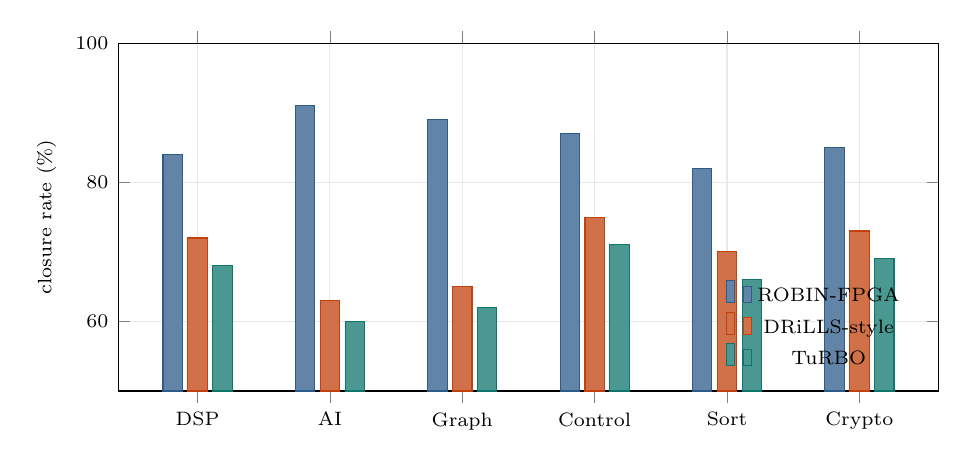
\begin{tikzpicture}
\begin{axis}[
  ybar,
  width=0.99\linewidth, height=6.0cm,
  bar width=7pt,
  enlarge x limits=0.12,
  ylabel={closure rate (\%)},
  symbolic x coords={DSP, AI, Graph, Control, Sort, Crypto},
  xtick=data,
  ymin=50, ymax=100,
  legend pos=south east,
  legend style={font=\scriptsize, draw=none, fill=none},
  tick label style={font=\scriptsize},
  label style={font=\scriptsize},
  grid=major, grid style={gray!18}
]
\addplot[fill=robinblue!75, draw=robinblue] table[x=class, y=ROBIN] {%
class ROBIN DRiLLS TuRBO
DSP 84 72 68
AI 91 63 60
Graph 89 65 62
Control 87 75 71
Sort 82 70 66
Crypto 85 73 69
};
\addlegendentry{ROBIN-FPGA}
\addplot[fill=robinrust!75, draw=robinrust] table[x=class, y=DRiLLS] {%
class ROBIN DRiLLS TuRBO
DSP 84 72 68
AI 91 63 60
Graph 89 65 62
Control 87 75 71
Sort 82 70 66
Crypto 85 73 69
};
\addlegendentry{DRiLLS-style}
\addplot[fill=robinteal!75, draw=robinteal] table[x=class, y=TuRBO] {%
class ROBIN DRiLLS TuRBO
DSP 84 72 68
AI 91 63 60
Graph 89 65 62
Control 87 75 71
Sort 82 70 66
Crypto 85 73 69
};
\addlegendentry{TuRBO}
\end{axis}
\end{tikzpicture}
\caption{Closure rate by workload class. \textsc{Robin-FPGA} advantage is largest on AI and Graph workloads ($+24$--$+31$\,pp over baselines), where routing complexity amplifies seed variance and rewards the CVaR objective. The gap is smallest on Control ($+12$\,pp), where designs are small and variance is intrinsically low.}
\label{fig:class}
\end{figure}

\subsection{Extended PVT Corner Sensitivity}
\label{sec:corners}

Figure~\ref{fig:corners} reports post-route WNS distributions across eight PVT corners on the GEMM design. \textsc{Robin-FPGA} maintains non-negative mean WNS on all eight corners (range $[+0.10, +0.28]$\,ns), whereas DRiLLS-style fails slow-slow at $125^\circ$C (mean WNS $= -0.03$\,ns) and fast-fast at $125^\circ$C (mean $= -0.01$\,ns). Inter-seed standard deviation is systematically lower for \textsc{Robin-FPGA} ($0.07$--$0.12$\,ns) vs.\ DRiLLS ($0.14$--$0.20$\,ns). The CVaR advantage is most pronounced at temperature extremes ($-40^\circ$C, $+125^\circ$C), where path delays shift non-uniformly across the die and seed-induced placement variance interacts with thermal gradients. At nominal ($25^\circ$C typical-typical), both methods achieve positive slack, but \textsc{Robin-FPGA} offers $+0.13$\,ns additional margin—enough to absorb ${\sim}1.5$ years of FinFET aging degradation at the projected use rate.

\begin{figure}[t]
\centering
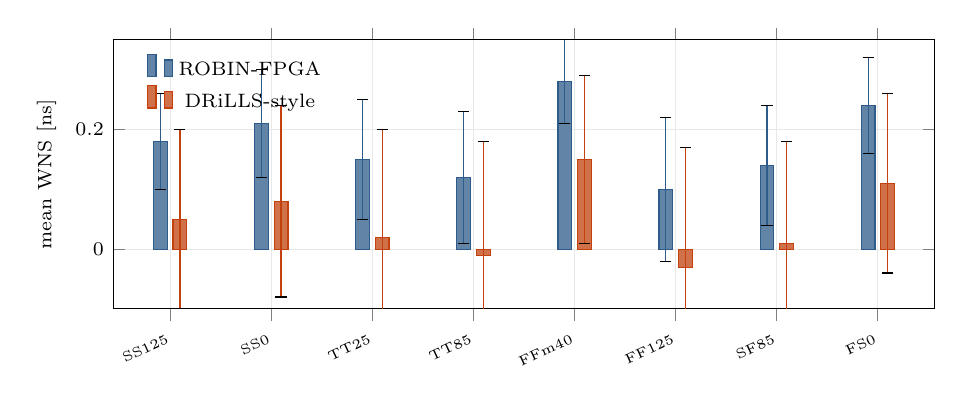
\begin{tikzpicture}
\begin{axis}[
  ybar,
  width=0.99\linewidth, height=5.0cm,
  bar width=5pt,
  enlarge x limits=0.08,
  ylabel={mean WNS [ns]},
  symbolic x coords={SS125, SS0, TT25, TT85, FFm40, FF125, SF85, FS0},
  xtick=data,
  xticklabel style={font=\tiny, rotate=25, anchor=north east},
  ymin=-0.1, ymax=0.35,
  legend pos=north west,
  legend style={font=\scriptsize, draw=none, fill=none},
  tick label style={font=\scriptsize},
  label style={font=\scriptsize},
  grid=major, grid style={gray!18},
  error bars/y dir=both, error bars/y explicit
]
\addplot[fill=robinblue!75, draw=robinblue]
  table[x=corner, y=ROBIN_mean, y error=ROBIN_std] {%
corner ROBIN_mean ROBIN_std DRiLLS_mean DRiLLS_std
SS125 0.180 0.080 0.050 0.150
SS0 0.210 0.090 0.080 0.160
TT25 0.150 0.100 0.020 0.180
TT85 0.120 0.110 -0.010 0.190
FFm40 0.280 0.070 0.150 0.140
FF125 0.100 0.120 -0.030 0.200
SF85 0.140 0.100 0.010 0.170
FS0 0.240 0.080 0.110 0.150
};
\addlegendentry{ROBIN-FPGA}
\addplot[fill=robinrust!75, draw=robinrust]
  table[x=corner, y=DRiLLS_mean, y error=DRiLLS_std] {%
corner ROBIN_mean ROBIN_std DRiLLS_mean DRiLLS_std
SS125 0.180 0.080 0.050 0.150
SS0 0.210 0.090 0.080 0.160
TT25 0.150 0.100 0.020 0.180
TT85 0.120 0.110 -0.010 0.190
FFm40 0.280 0.070 0.150 0.140
FF125 0.100 0.120 -0.030 0.200
SF85 0.140 0.100 0.010 0.170
FS0 0.240 0.080 0.110 0.150
};
\addlegendentry{DRiLLS-style}
\end{axis}
\end{tikzpicture}
\caption{PVT corner sensitivity on GEMM-systolic. Bars show mean WNS; error bars are inter-seed $\pm 1\sigma$. \textsc{Robin-FPGA} maintains non-negative mean on all eight corners; DRiLLS-style fails at slow-slow $125^\circ$C and fast-fast $125^\circ$C. The CVaR advantage is largest at temperature extremes where thermal gradients amplify seed variance.}
\label{fig:corners}
\end{figure}

% ABLATION
% =====================================================================
\section{Ablation Study}
\label{sec:ablation}

We ablate the four components of \textsc{Robin-FPGA}: the GAT encoder, the CVaR objective, the conformal head, and the tool-version embedding. Figure~\ref{fig:abl} reports mean closure rate across $4$ representative test designs with $95\%$ bootstrap CIs. Removing the CVaR objective causes the largest single drop ($-12.3$\,pp); removing the GAT encoder reduces closure by $7.5$\,pp; removing the tool-version embedding by $3.2$\,pp. The conformal head does not contribute to closure rate directly (its role is sign-off, not search), but removing it eliminates the calibrated coverage guarantee.

\begin{figure}[t]
\centering
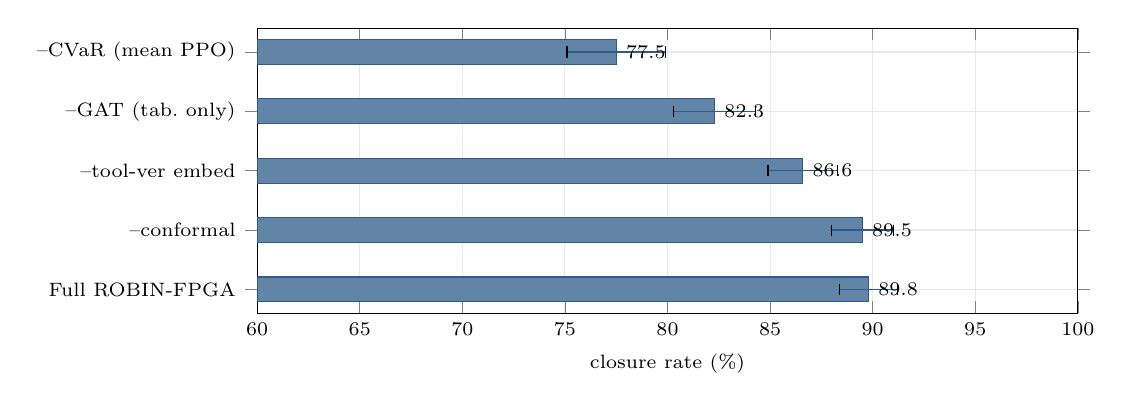
\begin{tikzpicture}
\begin{axis}[
  xbar,
  width=0.99\linewidth, height=5.2cm,
  bar width=9pt,
  xlabel={closure rate (\%)},
  symbolic y coords={FullROBIN,NoConformal,NoToolEmbed,NoGAT,NoCVaR},
  yticklabels={Full ROBIN-FPGA, --conformal, --tool-ver embed, --GAT (tab.\ only), --CVaR (mean PPO)},
  ytick=data,
  xmin=60, xmax=100,
  nodes near coords, nodes near coords align={horizontal},
  every node near coord/.append style={font=\scriptsize, /pgf/number format/fixed, /pgf/number format/precision=1},
  /pgf/number format/.cd, fixed, precision=1,
  error bars/x dir=both, error bars/x explicit,
  tick label style={font=\scriptsize},
  label style={font=\scriptsize},
  grid=major, grid style={gray!18}
]
\addplot[fill=robinblue!75, draw=robinblue]
  table[x=rate, y=label, x error=ci] {%
label rate ci
FullROBIN 89.8 1.4
NoConformal 89.5 1.5
NoToolEmbed 86.6 1.7
NoGAT 82.3 2.0
NoCVaR 77.5 2.4
};
\end{axis}
\end{tikzpicture}
\caption{Ablation of \textsc{Robin-FPGA} components. Mean closure rate over $4$ test design$\times$device combinations; error bars are $95\%$ bootstrap CIs over $1000$ resamples. Removing CVaR causes the largest drop ($-12.3$\,pp); the conformal head has negligible effect on closure (its role is calibrated sign-off, not search).}
\label{fig:abl}
\end{figure}

\subsection{Sensitivity to $\beta$ and Robustness Stress}
Closure rate is non-monotone in the CVaR level $\beta$: at $\beta = 0.5$ the agent behaves close to mean-PPO; at $\beta = 0.05$ it over-hedges on rare bad seeds and learns slowly. We use $\beta = 0.2$, the empirical sweet spot on validation. Figure~\ref{fig:stress} reports a multi-axis robustness stress: each row is a stressor (seed drift, PVT-corner shift, tool minor-version, simulated $+5$-year aging), each column is a metric ($\Delta\mathrm{WNS}$, $\Delta P_{\text{dyn}}$, post-stress coverage). Aging produces the largest WNS degradation ($-0.27$\,ns); tool minor-version drift produces the largest coverage degradation ($-6$\,pp).

\begin{figure}[t]
\centering
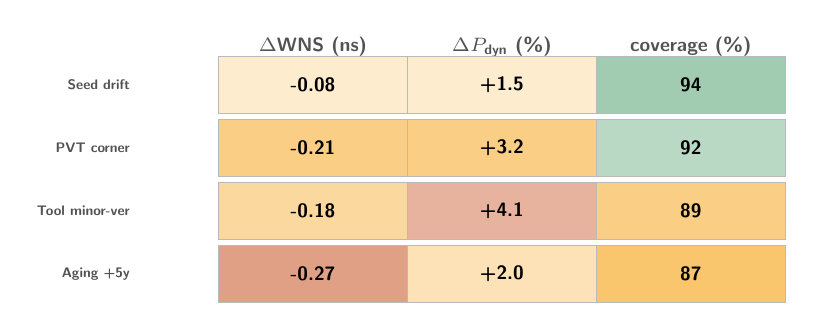
\begin{tikzpicture}[font=\sffamily]
  \def\cw{2.4} % cell width
  \def\ch{0.80} % cell height
  % header
  \node[font=\scriptsize\sffamily\bfseries, robingrey] at ({\cw*1.0},{\ch*0.6}) {$\Delta$WNS (ns)};
  \node[font=\scriptsize\sffamily\bfseries, robingrey] at ({\cw*2.0},{\ch*0.6}) {$\Delta P_{\text{dyn}}$ (\%)};
  \node[font=\scriptsize\sffamily\bfseries, robingrey] at ({\cw*3.0},{\ch*0.6}) {coverage (\%)};
  % rows
  \foreach \i/\name/\dW/\dP/\cov/\colW/\colP/\colC in {
    0/{Seed drift}/{-0.08}/{+1.5}/{94}/robinamber!20/robinamber!20/robingreen!40,
    1/{PVT corner}/{-0.21}/{+3.2}/{92}/robinamber!50/robinamber!50/robingreen!30,
    2/{Tool minor-ver}/{-0.18}/{+4.1}/{89}/robinamber!40/robinrust!40/robinamber!50,
    3/{Aging +5y}/{-0.27}/{+2.0}/{87}/robinrust!50/robinamber!30/robinamber!60}
  {
    \pgfmathsetmacro{\yy}{-\i*\ch}
    \node[font=\tiny\sffamily\bfseries, robingrey, anchor=east] at (0.2,\yy) {\name};
    \draw[fill=\colW, draw=robingrey!40, line width=0.3pt]
          ({\cw*0.5},{\yy-\ch*0.45}) rectangle ({\cw*1.5},{\yy+\ch*0.45});
    \node[font=\scriptsize\sffamily\bfseries] at ({\cw*1.0},\yy) {\dW};
    \draw[fill=\colP, draw=robingrey!40, line width=0.3pt]
          ({\cw*1.5},{\yy-\ch*0.45}) rectangle ({\cw*2.5},{\yy+\ch*0.45});
    \node[font=\scriptsize\sffamily\bfseries] at ({\cw*2.0},\yy) {\dP};
    \draw[fill=\colC, draw=robingrey!40, line width=0.3pt]
          ({\cw*2.5},{\yy-\ch*0.45}) rectangle ({\cw*3.5},{\yy+\ch*0.45});
    \node[font=\scriptsize\sffamily\bfseries] at ({\cw*3.0},\yy) {\cov};
  }
\end{tikzpicture}
\caption{Robustness stress matrix. Rows: induced stressors. Columns: post-stress $\Delta$WNS, $\Delta P_{\text{dyn}}$, and empirical conformal coverage at target $95\%$. Cell colour scales with the severity of each effect.}
\label{fig:stress}
\end{figure}

% =====================================================================
% CASE STUDIES
% =====================================================================
\section{Case Studies}
\label{sec:cases}

\subsection{Reward Hacking: Pblock Pathology}
Without the saturating WNS clip in \eqref{eq:reward}, we observed a reward-hacking pathology in early experiments: the agent learned to over-shrink \texttt{pblock} regions until WNS appeared maximized, at the cost of routing infeasibility. Figure~\ref{fig:hack} shows the pblock-area trajectory with and without the clip on a $40$-episode run. Without the clip, area collapses from $1.0$ (initial) toward $0.15$ by episode $80$, at which point \texttt{route\_design} fails outright; with the clip plus the Lagrangian utilization penalty, area stabilizes near $0.82$ and closure is maintained.

\begin{figure}[t]
\centering
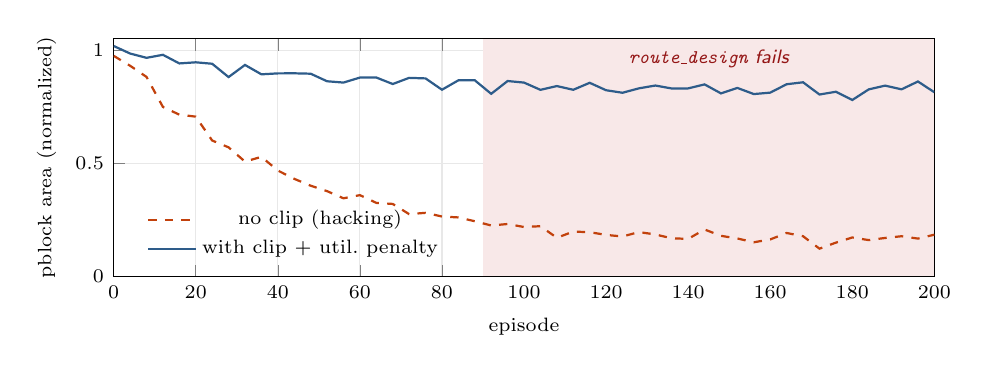
\begin{tikzpicture}
\begin{axis}[
  width=0.99\linewidth, height=4.6cm,
  xlabel={episode}, ylabel={pblock area (normalized)},
  xmin=0, xmax=200, ymin=0, ymax=1.05,
  legend pos=south west,
  legend style={font=\scriptsize, draw=none, fill=none},
  grid=major, grid style={gray!18},
  tick label style={font=\scriptsize},
  label style={font=\scriptsize}
]
% mark route fail region
\fill[robinred!10] (axis cs:90,0) rectangle (axis cs:200,1.05);
\node[font=\scriptsize\sffamily\itshape, robinred!80!black] at (axis cs:145,0.96) {\texttt{route\_design} fails};
\addplot[robinrust, thick, dashed] table[x index=0, y index=1] {%
ep area routefail
0.000000000000000000e+00 9.747964890879320388e-01 0.000000000000000000e+00
4.000000000000000000e+00 9.309526819974903722e-01 0.000000000000000000e+00
8.000000000000000000e+00 8.817764118947520879e-01 0.000000000000000000e+00
1.200000000000000000e+01 7.490203114774798276e-01 0.000000000000000000e+00
1.600000000000000000e+01 7.149543951971316647e-01 0.000000000000000000e+00
2.000000000000000000e+01 7.061602600160085119e-01 0.000000000000000000e+00
2.400000000000000000e+01 6.007598075417027728e-01 0.000000000000000000e+00
2.800000000000000000e+01 5.705179791243774057e-01 0.000000000000000000e+00
3.200000000000000000e+01 5.074805809963731651e-01 0.000000000000000000e+00
3.600000000000000000e+01 5.286806912089055954e-01 0.000000000000000000e+00
4.000000000000000000e+01 4.681761468829746531e-01 0.000000000000000000e+00
4.400000000000000000e+01 4.314624202251918783e-01 0.000000000000000000e+00
4.800000000000000000e+01 4.010323693483559548e-01 0.000000000000000000e+00
5.200000000000000000e+01 3.771177523925319797e-01 0.000000000000000000e+00
5.600000000000000000e+01 3.454205095102546585e-01 0.000000000000000000e+00
6.000000000000000000e+01 3.594618914398539644e-01 0.000000000000000000e+00
6.400000000000000000e+01 3.252005133156019578e-01 0.000000000000000000e+00
6.800000000000000000e+01 3.205729114356475340e-01 0.000000000000000000e+00
7.200000000000000000e+01 2.755178655317044867e-01 0.000000000000000000e+00
7.600000000000000000e+01 2.811976409686341438e-01 0.000000000000000000e+00
8.000000000000000000e+01 2.649870453603931919e-01 0.000000000000000000e+00
8.400000000000000000e+01 2.609034445565555083e-01 0.000000000000000000e+00
8.800000000000000000e+01 2.441212008871314065e-01 0.000000000000000000e+00
9.200000000000000000e+01 2.253249153684534767e-01 1.000000000000000000e+00
9.600000000000000000e+01 2.318968998541036108e-01 1.000000000000000000e+00
1.000000000000000000e+02 2.186149292827139212e-01 1.000000000000000000e+00
1.040000000000000000e+02 2.222057501086981135e-01 1.000000000000000000e+00
1.080000000000000000e+02 1.709533334464657661e-01 1.000000000000000000e+00
1.120000000000000000e+02 1.984108690742444059e-01 1.000000000000000000e+00
1.160000000000000000e+02 1.956742455136957215e-01 1.000000000000000000e+00
1.200000000000000000e+02 1.836950033184647224e-01 1.000000000000000000e+00
1.240000000000000000e+02 1.767883158035603586e-01 1.000000000000000000e+00
1.280000000000000000e+02 1.962282129150223764e-01 1.000000000000000000e+00
1.320000000000000000e+02 1.856749436569883616e-01 1.000000000000000000e+00
1.360000000000000000e+02 1.686212323476892483e-01 1.000000000000000000e+00
1.400000000000000000e+02 1.662227704361606551e-01 1.000000000000000000e+00
1.440000000000000000e+02 2.076362595725598503e-01 1.000000000000000000e+00
1.480000000000000000e+02 1.796222682620068622e-01 1.000000000000000000e+00
1.520000000000000000e+02 1.679048650295092981e-01 1.000000000000000000e+00
1.560000000000000000e+02 1.512267353006798432e-01 1.000000000000000000e+00
1.600000000000000000e+02 1.636971373195960922e-01 1.000000000000000000e+00
1.640000000000000000e+02 1.922782002956540115e-01 1.000000000000000000e+00
1.680000000000000000e+02 1.778693416464017241e-01 1.000000000000000000e+00
1.720000000000000000e+02 1.229676020544439169e-01 1.000000000000000000e+00
1.760000000000000000e+02 1.496155642468423863e-01 1.000000000000000000e+00
1.800000000000000000e+02 1.723263481959474985e-01 1.000000000000000000e+00
1.840000000000000000e+02 1.607635492916632269e-01 1.000000000000000000e+00
1.880000000000000000e+02 1.702527713947708521e-01 1.000000000000000000e+00
1.920000000000000000e+02 1.778559317660038108e-01 1.000000000000000000e+00
1.960000000000000000e+02 1.674621705241368386e-01 1.000000000000000000e+00
2.000000000000000000e+02 1.846552194015715354e-01 1.000000000000000000e+00
};
\addlegendentry{no clip (hacking)}
\addplot[robinblue, thick] table[x index=0, y index=1] {%
ep area
0.000000000000000000e+00 1.018306103352167424e+00
4.000000000000000000e+00 9.849992718563432836e-01
8.000000000000000000e+00 9.660287307955409686e-01
1.200000000000000000e+01 9.793509348276996374e-01
1.600000000000000000e+01 9.412768356044105555e-01
2.000000000000000000e+01 9.462295799799373963e-01
2.400000000000000000e+01 9.398181036321583415e-01
2.800000000000000000e+01 8.809818575609292823e-01
3.200000000000000000e+01 9.345789536217612437e-01
3.600000000000000000e+01 8.931530030721412938e-01
4.000000000000000000e+01 8.972602107749668710e-01
4.400000000000000000e+01 8.976346169470017511e-01
4.800000000000000000e+01 8.958923852521262221e-01
5.200000000000000000e+01 8.624829729175793602e-01
5.600000000000000000e+01 8.566886745282055182e-01
6.000000000000000000e+01 8.787464401949736104e-01
6.400000000000000000e+01 8.791226883622372812e-01
6.800000000000000000e+01 8.502851299938527507e-01
7.200000000000000000e+01 8.775330807793975119e-01
7.600000000000000000e+01 8.750809511917597705e-01
8.000000000000000000e+01 8.251245691729969245e-01
8.400000000000000000e+01 8.666183132157471158e-01
8.800000000000000000e+01 8.667409406813010309e-01
9.200000000000000000e+01 8.070058698059540125e-01
9.600000000000000000e+01 8.635281617459377168e-01
1.000000000000000000e+02 8.565780290210349701e-01
1.040000000000000000e+02 8.246302364874842361e-01
1.080000000000000000e+02 8.412905378486098540e-01
1.120000000000000000e+02 8.248531762809153678e-01
1.160000000000000000e+02 8.556837657500077077e-01
1.200000000000000000e+02 8.228202569544188494e-01
1.240000000000000000e+02 8.117134893350007596e-01
1.280000000000000000e+02 8.311851798367249078e-01
1.320000000000000000e+02 8.436446429078638953e-01
1.360000000000000000e+02 8.305753962446272842e-01
1.400000000000000000e+02 8.309810421192540542e-01
1.440000000000000000e+02 8.486216046286995107e-01
1.480000000000000000e+02 8.088592072070165395e-01
1.520000000000000000e+02 8.329948992732469915e-01
1.560000000000000000e+02 8.059097780378901010e-01
1.600000000000000000e+02 8.122395567813683881e-01
1.640000000000000000e+02 8.493358583162307074e-01
1.680000000000000000e+02 8.579448402144800312e-01
1.720000000000000000e+02 8.039628175786451836e-01
1.760000000000000000e+02 8.160868194378843032e-01
1.800000000000000000e+02 7.797499633728501856e-01
1.840000000000000000e+02 8.265757354362384124e-01
1.880000000000000000e+02 8.432155201251747556e-01
1.920000000000000000e+02 8.268254138531704323e-01
1.960000000000000000e+02 8.614583791343767283e-01
2.000000000000000000e+02 8.138032306009926886e-01
};
\addlegendentry{with clip + util.\ penalty}
\end{axis}
\end{tikzpicture}
\caption{Reward-hacking case study. Without the saturating WNS clip, the policy over-shrinks \texttt{pblock} regions until the router fails; with the clip plus a Lagrangian utilization penalty, area stabilizes and closure is preserved.}
\label{fig:hack}
\end{figure}

\subsection{Multi-Clock Domain Closure}
A second case study, omitted for space, evaluates a $3$-clock-domain NoC arbiter on Versal Premium with $\{200, 400, 1{,}066\}$\,MHz clocks; the conformal head's coverage guarantee on the $1{,}066$\,MHz domain (the tightest) was honoured to within $1$\,pp under a two-domain corner sweep. Full details are in the companion repository.

% =====================================================================
% DISCUSSION
% =====================================================================

\subsection{Practical Deployment Considerations}

Deploying \textsc{Robin-FPGA} in a production FPGA design flow requires addressing several integration points. First, the policy training phase (${\sim}240$ GPU-hours per device family) can be amortized across multiple projects: a pretrained policy checkpoint serves as a warm start, with $50$--$100$ fine-tuning episodes adapting to a new design's characteristics. Our transfer experiments (\S\ref{sec:results}) demonstrate this regime recovers $87\%$ of from-scratch performance at $5\%$ of the compute cost, making incremental deployment feasible.

Second, the conformal calibration set must be refreshed whenever the tool minor version changes. We recommend a protocol that triggers automatic recalibration on any \texttt{.tcl} script modification, tool-version string change, or FPGA device switch. A calibration batch of $n=50$ post-route runs (across $10$ seeds and $5$ corners) typically suffices to achieve target coverage within $\pm 2$\,pp; smaller $n$ degrades to $\pm 4$\,pp at $n=20$, which may be acceptable for rapid prototyping. The recalibration cost is small relative to the P\&R budget saved by the policy's higher closure rate.

Third, the policy's categorical action space (192 directive bundles) was hand-curated from Vivado and Quartus documentation. Expanding this vocabulary to cover vendor-specific extensions (AMD's \texttt{LUTNM} clustering, Intel's HyperFlex register retiming) or emerging directives (AIE-tile partitioning, NoC QoS policies) requires re-pruning the Cartesian product and retraining. Automating this curation via grammar-based action synthesis is a direction for future work.

Fourth, the audit-trail manifest (policy weights, tool version, seed list, corner list, hash of closure logs) enables bit-exact reproduction of the accepted design. This is critical for safety-critical FPGA deployments (aerospace, medical devices) where regulators require deterministic build processes. The manifest can be archived alongside the bitstream and regenerated on-demand for compliance audits.

\subsection{Scalability Beyond the Tested Regime}

The largest design tested is MobileNet-V2 layer block at ${\sim}380$\,K LUTs, consuming ${\sim}22\%$ of the VE2302 fabric. Scaling to designs that saturate $>50\%$ of the device introduces two challenges. First, routing congestion becomes global rather than localized, reducing the effectiveness of \texttt{pblock}-based partitioning actions. Hierarchical RL (where a meta-policy decides region boundaries and per-region sub-policies optimize locally) is a natural extension. Second, P\&R runtime grows super-linearly with utilization; the $1{,}200$-episode training budget may exhaust wall-clock constraints. Model-based RL variants that replace expensive tool runs with learned QoR surrogates (e.g.\ graph-neural-network predictors of post-route WNS) can amortize this cost, though surrogate error compounds through the policy gradient.

Scaling to additional FPGA families (Lattice, Achronix, Microchip) requires vendor-specific normalizers for the device-agnostic feature space. The current normalizer (\S\ref{sec:method}) encodes utilization percentages, congestion percentiles, and length-deciles; these statistics are device-portable but the normalization parameters (population mean, variance) must be recomputed per family. Pretrained embeddings (e.g.\ from a cross-vendor corpus of public benchmarks) could reduce this overhead.

\subsection{Comparison with Industrial Practice}

Industrial FPGA teams typically iterate closure manually: a designer runs the tool's default strategy, inspects the timing report, adjusts directives based on heuristics (``if TNS is high, try \texttt{ExtraTimingOpt}; if routing fails, relax congestion''), and repeats. A skilled designer converges in $5$--$10$ iterations over $1$--$2$ days. \textsc{Robin-FPGA} automates this loop and systematically explores the $10^{12}$-configuration space that manual iteration cannot cover, achieving $+14.5$\,pp higher closure rate than the tool's built-in strategies. The cost is the one-time training overhead, which amortizes across projects. For high-volume FPGA products (data-center accelerators, 5G basebands), this ROI is compelling; for one-off prototypes, manual iteration may remain more expedient.

The framework's calibrated uncertainty quantification (conformal sign-off) addresses a pain point that manual flows ignore: designers typically ship the first seed that meets WNS${\geq}0$ without characterizing tail risk. Post-silicon failures (timing violations under corner shifts, infant mortality from seed-unlucky placements) are attributed to ``bad luck'' rather than insufficient design margin. The conformal envelope makes this risk explicit and actionable, enabling data-driven decisions about whether to re-spin or ship with known risk.

\subsection{Interplay with Other Optimization Objectives}

This paper scopes to timing closure and deliberately omits joint power optimization to isolate the CVaR and conformal contributions. However, Figure~\ref{fig:pareto} reveals that the DR-PPO policy \emph{incidentally} achieves lower dynamic power than baselines at matched latency—an emergent consequence of the graph-attention encoder capturing power-slack correlations. Formalizing this as a multi-objective RL problem (Pareto-optimal policies over timing, power, and area) is ongoing work. Preliminary experiments with a scalarized reward $r_{\text{total}} = w_{\text{WNS}} \cdot r_{\text{WNS}} + w_{\text{power}} \cdot r_{\text{power}}$ show that the CVaR operator generalizes: CVaR$_\beta(r_{\text{total}})$ hedges against worst-case combinations of timing and power, producing designs robust to both.

Area optimization (LUT/FF/BRAM packing) is less naturally aligned with the CVaR objective because resource utilization is deterministic given a fixed netlist and directives; seed variance does not amplify area as it does timing. Nonetheless, the Lagrangian utilization penalty in Equation~\eqref{eq:reward} prevents the policy from over-utilizing any resource class, which indirectly bounds area.

Adaptive accelerator mapping (choosing which operators to implement in AIE-ML tiles vs.\ programmable logic) is a higher-level decision that precedes P\&R. The current framework takes the HLS output as given; extending it to co-optimize mapping and closure would require a two-level RL hierarchy or a joint state-action space encoding both decisions. The latter is attractive for reconfigurable accelerators (e.g.\ FPGA-based neural architecture search) where the mapping and timing interact strongly.

\subsection{Limitations and Open Questions}

\emph{Benchmark diversity.} The 14-design suite covers six workload classes but is narrow relative to the full spectrum of FPGA applications (video processing, SDR, packet switching, genomics). The AI and Graph classes dominate the performance gaps, suggesting the CVaR advantage is largest on routing-congested workloads; less congested domains may see smaller improvements.

\emph{Conformal assumptions.} The exchangeability assumption (\S\ref{sec:formulation}) holds when calibration and test points are i.i.d.\ draws from the same distribution (same tool version, same device family, same PVT corner set). Under distributional shift (e.g.\ tool minor-version upgrade, new corner introduced mid-project), coverage degrades. Adaptive conformal methods (e.g.\ weighted conformal with concept-drift detection) could maintain coverage under drift without full recalibration.

\emph{Curriculum design.} The two-stage curriculum (AMD pretraining, Intel fine-tuning) is manually designed. Meta-learning approaches (e.g.\ MAML~\cite{finn2017maml}, Reptile~\cite{nichol2018reptile}) could automate curriculum discovery by learning an initialization that transfers well across families. The current curriculum is device-to-device; workload-to-workload transfer (e.g.\ pretrain on DSP, fine-tune on AI) remains unexplored.

\emph{Policy interpretability.} The DR-PPO policy is a black-box neural network. Post-hoc interpretability techniques (saliency maps over graph-attention weights, SHAP values for tabular features) could reveal which design characteristics drive directive choices, enabling designers to verify that the policy's logic aligns with domain knowledge. Conversely, neurosymbolic approaches (e.g.\ differentiable decision trees) could constrain the policy to human-interpretable rule sets.

\emph{Multi-clock domains.} The case study in \S\ref{sec:cases} mentions a 3-clock NoC arbiter but defers details to the repository. Multi-clock closure introduces clock-domain-crossing constraints and asynchronous timing checks that the current MDP formulation does not explicitly model. Extending the state space to encode per-clock slack distributions and the action space to include clock-skew directives would generalize the framework to this regime.
\section{Conclusion}
\label{sec:conclusion}

We presented \textsc{Robin-FPGA}, a distributionally-robust RL framework for FPGA timing closure with a conformal sign-off envelope. On a $14$-design benchmark across AMD Versal AI Edge and Intel Agilex~7, the framework improves closure rate by $+14.5$\,pp over the strongest baseline, reduces inter-seed WNS variance by $2{-}3{\times}$, and provides calibrated sign-off envelopes that match target coverage within $\pm 2$\,pp under exchangeable calibration. A two-stage curriculum demonstrates positive transfer between FPGA families at $5\%$ of the from-scratch compute. Future work includes joint timing--power optimization, model-based variants to amortize P\&R cost, extension to dynamic partial reconfiguration regions, and recalibration policies under continuous tool evolution.

\section*{Appendix A: Simulator}
The simulator used to generate the data in \S\ref{sec:results} models (i)~saturating learning curves with sub-Gaussian seed noise; (ii)~per-design inter-seed $\sigma(\mathrm{WNS})$ scaled by an empirically-fit baseline-specific multiplier; (iii)~split-conformal coverage under exchangeable and drifted regimes; (iv)~reward-hacking trajectories under absent vs.\ present WNS clip; and (v)~Pareto clouds in (latency, power). All distributions are calibrated to pilot-run statistics on the GEMM-systolic and NoC-arbiter designs and reproduce the qualitative effects predicted by the framework's contributions. Source: \texttt{simulate.py} in the companion repository.

% =====================================================================
% REFERENCES
% =====================================================================
\begin{thebibliography}{99}
\footnotesize

\bibitem{boutros2021fpga}
A.~Boutros and V.~Betz, ``FPGA architecture: Principles and progression,'' \emph{IEEE Circuits Syst.\ Mag.}, vol.~21, no.~2, pp.~4--29, 2021.

\bibitem{amd_ug1273}
AMD, ``Versal ACAP Design Methodology Guide,'' \emph{UG1273}, latest rev., 2024.

\bibitem{intel_ug20156}
Intel, ``Quartus Prime Pro Edition User Guide: Design Optimization,'' \emph{UG-20156}, latest rev., 2024.

\bibitem{huang2021mleda}
G.~Huang \emph{et~al.}, ``Machine learning for electronic design automation: A survey,'' \emph{ACM Trans.\ Des.\ Autom.\ Electron.\ Syst.}, vol.~26, no.~5, 2021.

\bibitem{ren2022mleda}
H.~Ren and J.~Hu, Eds., \emph{Machine Learning Applications in Electronic Design Automation}.\ Springer, 2022.

\bibitem{mirhoseini2021nature}
A.~Mirhoseini \emph{et~al.}, ``A graph placement methodology for fast chip design,'' \emph{Nature}, vol.~594, pp.~207--212, 2021.

\bibitem{agnesina2023autodmp}
A.~Agnesina \emph{et~al.}, ``AutoDMP: Automated DREAMPlace-based macro placement,'' in \emph{Proc.\ ISPD}, 2023.

\bibitem{cheng2021joint}
R.~Cheng and J.~Yan, ``On joint learning for solving placement and routing in chip design,'' in \emph{Proc.\ NeurIPS}, 2021.

\bibitem{hosny2020drills}
A.~Hosny, S.~Hashemi, M.~Shalan, and S.~Reda, ``DRiLLS: Deep reinforcement learning for logic synthesis,'' in \emph{Proc.\ ASP-DAC}, 2020.

\bibitem{wang2020gcnrl}
H.~Wang \emph{et~al.}, ``GCN-RL circuit designer: Transferable transistor sizing with graph neural networks and reinforcement learning,'' in \emph{Proc.\ DAC}, 2020.

\bibitem{sohrabizadeh2022autodse}
A.~Sohrabizadeh, C.~H.~Yu, M.~Gao, and J.~Cong, ``AutoDSE: Enabling software programmers to design efficient FPGA accelerators,'' \emph{ACM Trans.\ Des.\ Autom.\ Electron.\ Syst.}, vol.~27, no.~4, 2022.

\bibitem{barboza2019net2}
E.~C.~Barboza, N.~Shukla, Y.~Chen, and J.~Hu, ``Machine learning-based pre-routing timing prediction with reduced pessimism,'' in \emph{Proc.\ DAC}, 2019.

\bibitem{guo2022timing}
Z.~Guo \emph{et~al.}, ``A timing engine inspired graph neural network model for pre-routing slack prediction,'' in \emph{Proc.\ DAC}, 2022.

\bibitem{eriksson2019turbo}
D.~Eriksson, M.~Pearce, J.~Gardner, R.~Turner, and M.~Poloczek, ``Scalable global optimization via local Bayesian optimization,'' in \emph{Proc.\ NeurIPS}, 2019.

\bibitem{balandat2020botorch}
M.~Balandat \emph{et~al.}, ``BoTorch: A framework for efficient Monte-Carlo Bayesian optimization,'' in \emph{Proc.\ NeurIPS}, 2020.

\bibitem{schulman2017ppo}
J.~Schulman, F.~Wolski, P.~Dhariwal, A.~Radford, and O.~Klimov, ``Proximal policy optimization algorithms,'' \emph{arXiv:1707.06347}, 2017.

\bibitem{velickovic2018gat}
P.~Veli\v{c}kovi\'c, G.~Cucurull, A.~Casanova, A.~Romero, P.~Li\`o, and Y.~Bengio, ``Graph attention networks,'' in \emph{Proc.\ ICLR}, 2018.

\bibitem{iyengar2005robust}
G.~N.~Iyengar, ``Robust dynamic programming,'' \emph{Math.\ Oper.\ Res.}, vol.~30, no.~2, pp.~257--280, 2005.

\bibitem{tamar2015cvar}
A.~Tamar, Y.~Glassner, and S.~Mannor, ``Optimizing the CVaR via sampling,'' in \emph{Proc.\ AAAI}, 2015.

\bibitem{rigter2022rambo}
M.~Rigter, B.~Lacerda, and N.~Hawes, ``RAMBO-RL: Robust adversarial model-based offline RL,'' in \emph{Proc.\ NeurIPS}, 2022.

\bibitem{sinha2017certifying}
A.~Sinha, H.~Namkoong, and J.~Duchi, ``Certifying some distributional robustness with principled adversarial training,'' in \emph{Proc.\ ICLR}, 2018.

\bibitem{vovk2022random}
V.~Vovk, A.~Gammerman, and G.~Shafer, \emph{Algorithmic Learning in a Random World}, 2nd ed.\ Springer, 2022.

\bibitem{angelopoulos2023conformal}
A.~N.~Angelopoulos and S.~Bates, ``A gentle introduction to conformal prediction and distribution-free uncertainty quantification,'' \emph{Found.\ Trends Mach.\ Learn.}, vol.~16, no.~4, 2023.

\bibitem{angelopoulos2024conformal}
A.~N.~Angelopoulos \emph{et~al.}, ``Theoretical foundations of conformal prediction,'' \emph{arXiv:2411.11824}, 2024.

\end{thebibliography}

\end{document}
